\chapter[red]{Classes}
\label{chap:Classes}
\chapterimage
\thispagestyle{plain}

\begin{multicols*}{2}
Even with the same amount of experience, not all player characters are the same. Although they are all assumed to be adventurers, their backgrounds may be rather different from each other. For example a young human that has just finished a five-year apprenticeship under a wizard and has now mastered the essentials of spellcasting is going to be very different than a dwarven warrior who has spent every weekend doing combat training in case of goblin attack.

In the game, this difference in background, upbringing and training is represented by classes. Each player character (and some important non-player characters, if they are also adventurers) has a class based on their background. As a player, you have a free choice of class for your character, providing your ability scores meet some minimum criteria.

The character’s class determines which sorts of weapon and armor they will have been trained how to use, and also may provide them with various special abilities. There is little difference between the classes at low levels, since all the characters are novices in their chosen professions. However, as characters gain experience and levels, the differences between the classes become more pronounced.

Dark Dungeons has six different classes for human adventurers and four classes for non-human adventurers. Non-humans have different cultures to humans and different natural abilities, so their adventurers are brought up with different backgrounds and are sufficiently different from human adventurers to warrant their own classes.

The six human classes are \iref[class:Cleric]{Cleric}, \iref[class:Druid]{Druid}, \iref[class:Fighter]{Fighter}, \iref[class:Monk]{Monk}, \iref[class:Rogue]{Rogue}, \iref[class:Wizard]{Wizard}, and the non-human ones are \iref[class:Dwarf]{Dwarf}, \iref[class:Elf]{Elf}, \iref[class:Gnome]{Gnome}, and \iref[class:Halfling]{Halfling}.

\section{Subclasses}\index[general]{Subclasses}
Some classes have subclasses which can be chosen in place of the class. These subclasses are more specialized versions of the class, with changes made to better suit this specialization. Other than these changes, the subclass functions identically to the class.

Unless stated otherwise, choosing a subclass must be done during character creation. Some subclasses can not be chosen until a specified level. Once a subclass is chosen it may not be dropped nor swapped for another subclass.

Subclasses can be found at the end of the class description.

\section{Class Format}\index[general]{Class Format}\label{sec:Class Format}
Each class description contains a stat block containing some or all of the following entries.

\textbf{Ability Requirements:} These are the minimum ability scores required to choose this class.

\textbf{Prime Requisite:} This is the ability score most relevant to the class (see \fullref{sec:Prime Requisite}).

\textbf{Ability Modifiers:} Some demi-humans naturally excel or fall short in some of their abilities. This lists the adjustments made to these abilities to reflect that.

\textbf{Hit Dice:} This is the amount and type of die rolled each level up to \nth{9} to determine the character’s hit points (see \fullref{sec:Hit Points}). The character’s \iref[sec:Constitution]{Constitution} bonus is added to each of these rolls. The results are cumulative, so a \nth{6} level \iref[class:Dwarf]{Dwarf} has 6d8 hit points. After \nth{9} level, the character no longer roll for hit points with \iref[sec:Constitution]{Constitution} bonuses. Instead, they gain 1 hit point per level, unless the die type is a d8 in which case they gain 2.

\textbf{Movement:} This shows how many feet per rounds a member of this class can move. If the class has unusual forms of movement, such as being able to burrow or fly, these will also be listed.

\textbf{Weapons:} This is a list of weapons that a member of this class are able to use. Weapons restrictions are typically due to size of the weapon which impedes the use of special abilities or in the case of some demi-humans are too large for their small stature.

\textbf{Natural AC:} This is the character’s armor class (see \fullref{sec:Armor Class}) while not wearing any armor and without their \iref[sec:Dexterity]{Dexterity} modifier. The natural armor class may be from tough skin, great agility, or martial training.

\textbf{Armor:} This is a list of armor that a member of this class are able to use. Armor restrictions are typically imposed due to armor interfering with special abilities that require precise movement.

\textbf{Special Abilities:} This is a list of special abilities gained by choosing this class. They are sorted alphabetically by the level in which they are gained.

\textbf{Bonus Skills:} Some classes start with certain skills without expending skill points. This list those skills.

\textbf{Required Skills:} Some classes are required to take certain skills. This list those skills. The character must use their first available skill points to acquire these.

\textbf{Experience:} This lists the amount of experience points needed to gain a level (see \fullref{sec:Gaining Levels}). For example, a \nth{5} level \iref[class:Elf]{Elf} needs 64,000 experience points to reach \nth{6} level.

\textbf{Hit Points:} Some classes receive hit points based directly on their level rather than on their hit dice. This lists the amount of hit points gained. These classes do not get to add their \iref[sec:Constitution]{Constitution} bonus to their hit point total.

\textbf{Attack Bonus:} The character’s attack bonus is based on their level. See \fullref{sec:Attack Bonus} for details of how this translates into to-hit numbers for different armor classes.

\textbf{Saving Throws:} These are the target difficulties that the character uses when making saving throws (see \fullref{sec:Saving Throws}).

\textbf{Special:} This shows when special abilities, skill points (see \fullref{chap:Skills}), and weapon feats (see \fullref{chap:Weapon Feats}) are gained.

\section{Cleric}\index[classes]{Cleric}\label{class:Cleric}
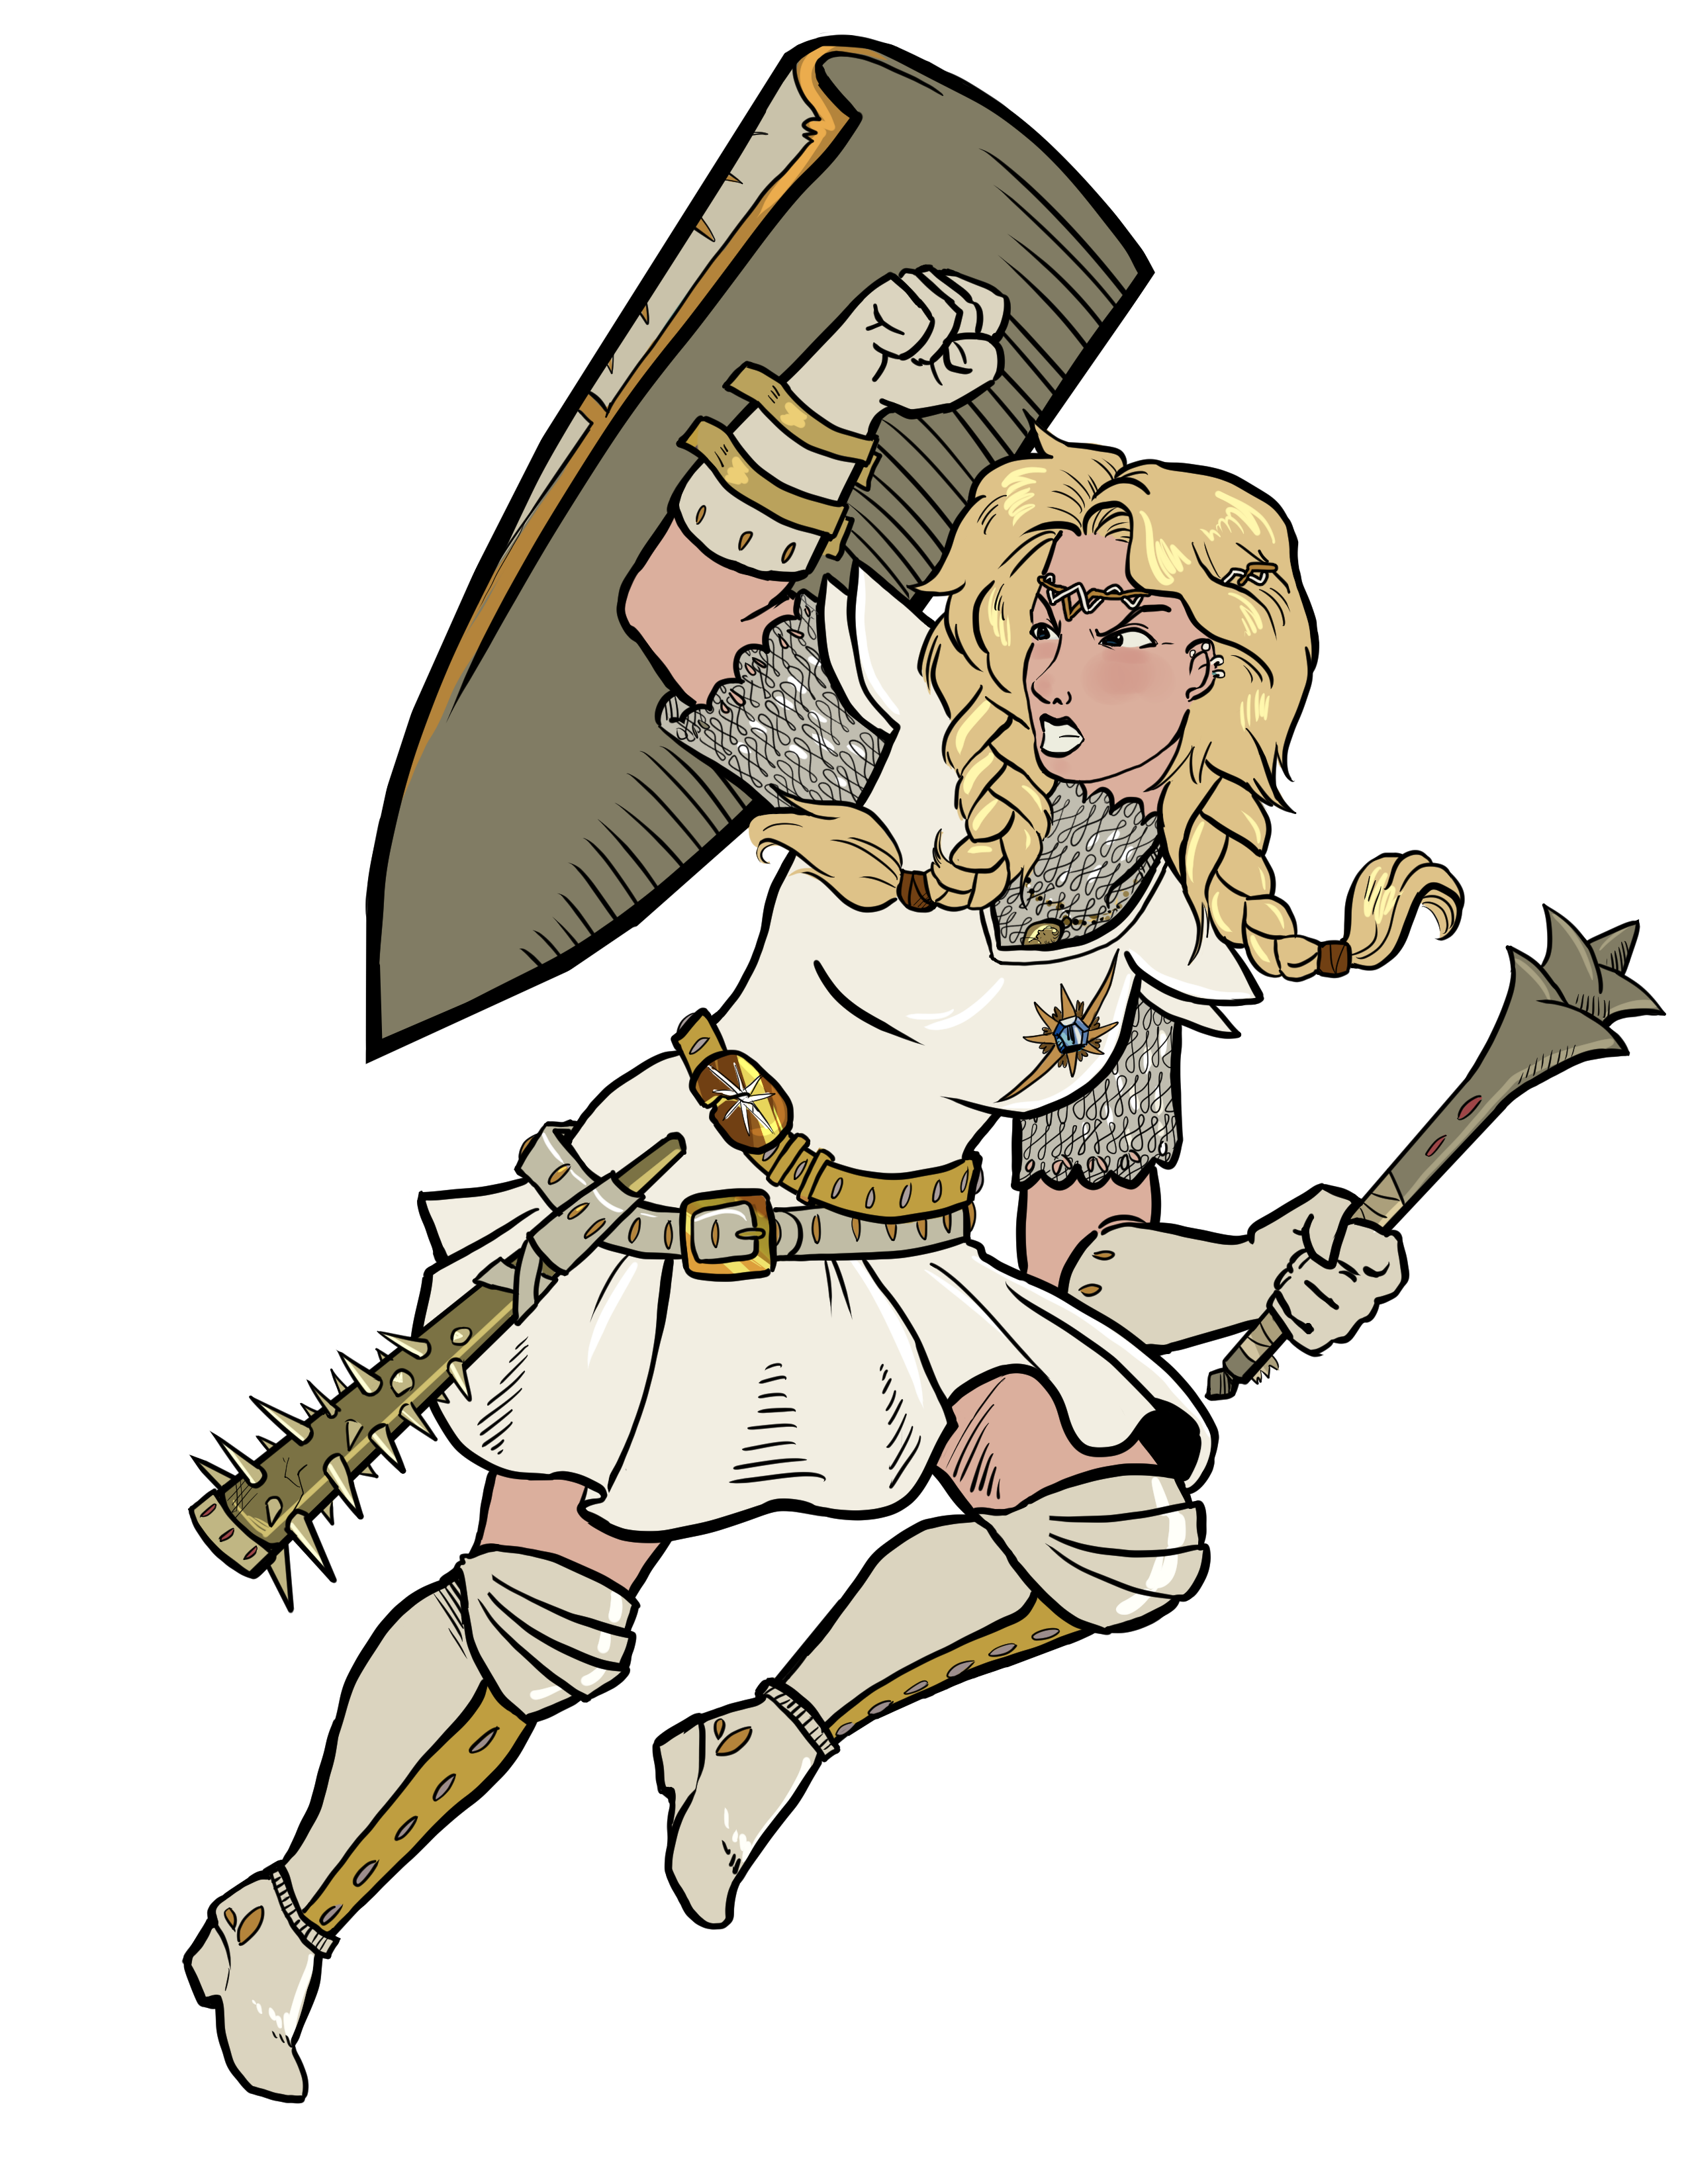
\includegraphics[width=\columnwidth]{Classes/Cleric}
Clerics are human characters who have devoted themselves to religious service.

In exchange for taking vows to uphold their religion’s principles and tenets and to never use bladed weapons, clerics gain the ability to drive away or even destroy undead creatures; and to cast clerical spells.

Depending on the particular religion the cleric follows, the cleric may worship one or more gods—or even an entire pantheon of gods. Other religions involve the worship of abstract concepts such as “fire” or “good”, or involve the worship of ancestral or other spirits. Yet other religions are based on abstract philosophies.

Regardless of the type of religion, the powers wielded by a cleric are actually provided by an individual \iref[chap:Immortals]{Immortal}. It is up to the Game Master to determine the exact details of the religion and what role the \iref[chap:Immortals]{Immortal} plays in it. Commonly this role will be as an intermediary, servant or messenger of the god(s) that the cleric worships.

With the Game Master’s permission, it is even possible for a cleric to be completely non-religious—having been given clerical power by an \iref[chap:Immortals]{Immortal} as part of some other more business-like arrangement.

Within an adventuring party, clerics tend to operate in a support role. Their spells emphasize healing and protection rather than flashy attacks.

\subsection{Abilities}
\textbf{Turn Undead:}\index[general]{Turn Undead} Clerics have the ability to channel divine power from their patron in order to drive away or even destroy undead creatures such as zombies or vampires.

When your cleric tries to turn undead, you must first decide which undead you are targeting. If you are facing a mixed group of undead you can only turn one type of undead each round.

Once you have decided which undead you wish to attempt to turn, consult \fullref{tab:Turning Undead by Cleric Level} and compare your cleric’s level with the type of undead that you are trying to turn. The entry in the table will indicate the level of success, as follows:

‘-’ —You are not powerful enough to turn this type of undead.

‘11’—Roll 2d6. Your attempt at turning the undead will be successful if you roll an 11 or higher. If the roll fails, you will not be able to try to turn these same undead again during this fight.

If the roll succeeds then roll 2d6 to see how many of the undead are affected. Targeted undead with a total number of hit dice equal to this roll will be turned, with the exception that at least one undead will always be affected even if it has more hit dice than the roll.

‘9’—Roll 2d6. Your attempt at turning the undead will be successful if you roll a 9 or higher. If the roll fails, you will not be able to try to turn these same undead again during this fight.

If the roll succeeds then roll 2d6 to see how many of the undead are affected. Targeted undead with a total number of hit dice equal to this roll will be turned, with the exception that at least one undead will always be affected even if it has more hit dice than the roll.

‘7’—Roll 2d6. Your attempt at turning the undead will be successful if you roll a 7 or higher. If the roll fails, you will not be able to try to turn these same undead again during this fight.

If the roll succeeds then roll 2d6 to see how many of the undead are affected. Targeted undead with a total number of hit dice equal to this roll will be turned, with the exception that at least one undead will always be affected even if it has more hit dice than the roll.

‘t’—Your attempt at turning the undead automatically succeeds. Roll 2d6 to see how many undead are affected.

Targeted undead with a total number of hit dice equal to this roll will be turned, with the exception that at least one will always be affected even if it has more hit dice than the roll.

‘d’—Your attempt at turning the undead is automatically successful, and will destroy the undead rather than simply turning them. Roll 2d6 to see how many of the undead are affected.

Targeted undead with a total number of hit dice equal to this roll will be destroyed, with the exception that at least one undead will always be affected even if it has more hit dice than the roll.

‘D’—Your attempt at turning the undead is automatically successful, and will destroy the undead rather than simply turning them. Roll 3d6 to see how many of the undead are affected.

Targeted undead with a total number of hit dice equal to this roll will be destroyed, with the exception that at least one undead will always be affected even if it has more hit dice than the roll.

‘X’—Your attempt at turning the undead is automatically successful, and will destroy the undead rather than simply turning them. Roll 4d6 to see how many of the undead are affected.

Targeted undead with a total number of hit dice equal to this roll will be destroyed, with the exception that at least one undead will always be affected even if it has more hit dice than the roll.

Undead that have been turned will be compelled to flee from the cleric as fast as they are able for at least five minutes.

If cornered during this time, they will cower and be unable to make any kind of attack, although intelligent undead may use whatever defensive powers they possess in order to protect themselves. The bodies of undead that have been destroyed will crumble to a fine ash, and incorporeal undead will fade away to nothing.

Some particularly powerful undead might have ways of resisting being turned, and a powerful master may be able to protect their minions making them harder to turn.

\example{Elfstar the second level cleric is facing a pack of zombies. On her action she decides to use her Turn Undead ability rather than attacking with her mace.

Elfstar’s player announces that she is targeting the zombies with her turn attempt, and looks on her character sheet (onto which she has copied the relevant information from).

This shows a ‘7’, so she needs to roll 2d6 and get a 7 or higher to successfully turn the zombies. She rolls the dice and gets a 10—success!

Elfstar’s player now rolls 2d6 a second time to see how many zombies Elfstar has just turned. She rolls a 9. Since zombies have two hit dice each, Elfstar has successfully turned four of the zombies (a total of 8 hit dice). She cannot turn a fifth one, since that would be a total of 10 hit dice which is higher than her roll of 9).}

\textbf{Spells:} Starting at \nth{2} level, clerics can cast clerical spells. See \fullref{sec:Spell Descriptions} for detailed descriptions of these spells.

Providing a cleric has had a good night’s sleep (8 hours), they can spend an hour meditating and/or performing religious rites after waking up in order to gain spells for the day as indicated on \fullref{tab:Cleric Spells per Day by Spell Level}.

Every cleric has access to all cleric spells of levels they can cast, and chooses freely which ones to prepare each day within the limits of the numbers shown on \fullref{tab:Cleric Spells per Day by Spell Level}.

Each prepared spell can be cast once during the day, and if a cleric wishes to cast a spell more than once then they must prepare the spell more than once, taking up multiple spell slots of the spell’s level.

Some clerical spells are reversible. These spells can be reversed in order to have an effect opposite to the normal effect of the spell. A cleric chooses whether or not to reverse the spell at the time of casting, not at the time of preparation. Clerical spells are always prepared in their normal form.

See \fullref{chap:Spells and Spellcasting} for more information on spells and spellcasting.

\statblock{\textbf{Ability Requirements:} Wisdom 9

\textbf{Prime Requisite:} Wisdom

\textbf{Hit Dice:} 1d6

\textbf{Movement:} 40 feet

\textbf{Weapons:} Any blunt

\textbf{Armor:} Any

\textbf{Special Abilities:} Spells, Turn Undead}

\end{multicols*}
\begin {table}[H]
  \caption{Cleric Progression}
	\begin{tabularx}{\columnwidth}{>{\bfseries}cccM{.31in}M{.51in}M{.25in}M{.43in}M{.32in}M{.45in}Y}
		\thead{}&\thead{}&\thead{}&\thead{}&\multicolumn{5}{c}{\thead{Saving Throws}}\thead{}&\setcounter{rownum}{0}\\
		\thead{Level} & \thead{Experience} & \thead{Hit Dice} & \thead{Attack Bonus} & \thead{Death Ray/ Poison} & \thead{Magic Wands} & \thead{Paralysis/ Petrify} & \thead{Breath Weapon} & \thead{Rod/Staff/ Spell} & \thead{Special}\\
		1 & 0 & 1d6 & +1 & 11 & 12 & 14 & 16 & 15 & Turn Undead, +4 Skill Points, +2 Weapon Feats\\
		2 & 1,500 & 2d6 & +1 & 11 & 12 & 14 & 16 & 15 & Spells\\
		3 & 3,000 & 3d6 & +1 & 11 & 12 & 14 & 16 & 15 & +1 Weapon Feat\\
		4 & 6,000 & 4d6 & +2 & 10 & 11 & 13 & 15 & 14 & -\\
		5 & 12,000 & 5d6 & +2 & 10 & 11 & 13 & 15 & 14 & +1 Skill Point\\
		6 & 25,000 & 6d6 & +3 & 9 & 10 & 12 & 14 & 13 & +1 Weapon Feat\\
		7 & 50,000 & 7d6 & +3 & 9 & 10 & 12 & 14 & 13 & -\\
		8 & 100,000 & 8d6 & +4 & 8 & 9 & 11 & 13 & 12 & -\\
		9 & 200,000 & 9d6 & +4 & 8 & 9 & 11 & 13 & 12 & +1 Skill Point, +1 Weapon Feat\\
		10 & 300,000 & 9d6+1 & +5 & 7 & 8 & 10 & 12 & 11 & -\\
		11 & 400,000 & 9d6+2 & +5 & 7 & 8 & 10 & 12 & 11 & +1 Weapon Feat\\
		12 & 500,000 & 9d6+3 & +6 & 7 & 8 & 9 & 11 & 10 & -\\
		13 & 600,000 & 9d6+4 & +6 & 6 & 7 & 9 & 11 & 10 & +1 Skill Point\\
		14 & 700,000 & 9d6+5 & +7 & 6 & 7 & 8 & 10 & 9 & -\\
		15 & 800,000 & 9d6+6 & +7 & 6 & 7 & 8 & 10 & 9 & +1 Weapon Feat\\
		16 & 900,000 & 9d6+7 & +8 & 6 & 7 & 7 & 9 & 8 & -\\
		17 & 1,000,000 & 9d6+8 & +8 & 5 & 7 & 7 & 9 & 8 & +1 Skill Point\\
		18 & 1,100,000 & 9d6+9 & +9 & 5 & 7 & 6 & 8 & 7 & -\\
		19 & 1,200,000 & 9d6+10 & +9 & 5 & 7 & 6 & 8 & 7 & -\\
		20 & 1,300,000 & 9d6+11 & +10 & 5 & 6 & 6 & 7 & 6 & -\\
		21 & 1,400,000 & 9d6+12 & +10 & 4 & 6 & 5 & 7 & 6 & +1 Skill Point\\
		22 & 1,500,000 & 9d6+13 & +11 & 4 & 5 & 5 & 6 & 5 & -\\
		23 & 1,600,000 & 9d6+14 & +11 & 4 & 5 & 5 & 6 & 5 & +1 Weapon Feat\\
		24 & 1,700,000 & 9d6+15 & +12 & 4 & 5 & 5 & 5 & 5 & -\\
		25 & 1,800,000 & 9d6+16 & +12 & 3 & 4 & 4 & 5 & 4 & +1 Skill Point\\
		26 & 1,900,000 & 9d6+17 & +13 & 3 & 4 & 4 & 4 & 4 & -\\
		27 & 2,000,000 & 9d6+18 & +13 & 3 & 4 & 4 & 4 & 4 & -\\
		28 & 2,100,000 & 9d6+19 & +14 & 3 & 4 & 4 & 4 & 4 & -\\
		29 & 2,200,000 & 9d6+20 & +14 & 2 & 3 & 3 & 3 & 3 & +1 Skill Point\\
		30 & 2,300,000 & 9d6+21 & +15 & 2 & 3 & 3 & 3 & 3 & +1 Weapon Feat\\
		31 & 2,400,000 & 9d6+22 & +15 & 2 & 3 & 3 & 3 & 3 & -\\
		32 & 2,500,000 & 9d6+23 & +16 & 2 & 3 & 3 & 3 & 3 & -\\
		33 & 2,600,000 & 9d6+24 & +16 & 2 & 2 & 2 & 2 & 2 & +1 Skill Point\\
		34 & 2,700,000 & 9d6+25 & +17 & 2 & 2 & 2 & 2 & 2 & -\\
		35 & 2,800,000 & 9d6+26 & +17 & 2 & 2 & 2 & 2 & 2 & -\\
		36 & 2,900,000 & 9d6+27 & +18 & 2 & 2 & 2 & 2 & 2 & +1 Weapon Feat\
  \end {tabularx}
\end {table}
\newpage
\begin{multicols*}{2}

\begin {table}[H]
  \caption{Cleric Spells per Day by Spell Level}\label{tab:Cleric Spells per Day by Spell Level}
  \begin{tabularx}{\columnwidth}{>{\bfseries}YYYYYYYY}
		\thead{} & \multicolumn{7}{c}{\thead{Spell Level}}\\
		\thead{Level} & \thead{1} & \thead{2} & \thead{3} & \thead{4} & \thead{5} & \thead{6} & \thead{7}\\
		1 & - & - & - & - & - & - & -\\
		2 & 1 & - & - & - & - & - & -\\
		3 & 2 & - & - & - & - & - & -\\
		4 & 2 & 1 & - & - & - & - & -\\
		5 & 2 & 2 & - & - & - & - & -\\
		6 & 2 & 2 & 1 & - & - & - & -\\
		7 & 3 & 2 & 2 & - & - & - & -\\
		8 & 3 & 3 & 2 & 1 & - & - & -\\
		9 & 3 & 3 & 3 & 2 & - & - & -\\
		10 & 4 & 4 & 3 & 2 & 1 & - & -\\
		11 & 4 & 4 & 3 & 3 & 2 & - & -\\
		12 & 4 & 4 & 4 & 3 & 2 & 1 & -\\
		13 & 5 & 5 & 4 & 3 & 2 & 2 & -\\
		14 & 5 & 5 & 5 & 3 & 3 & 2 & -\\
		15 & 6 & 5 & 5 & 3 & 3 & 3 & -\\
		16 & 6 & 5 & 5 & 4 & 4 & 3 & -\\
		17 & 6 & 6 & 5 & 4 & 4 & 3 & 1\\
		18 & 6 & 6 & 5 & 4 & 4 & 3 & 2\\
		19 & 7 & 6 & 5 & 4 & 4 & 4 & 2\\
		20 & 7 & 6 & 5 & 4 & 4 & 4 & 3\\
		21 & 7 & 6 & 5 & 5 & 5 & 4 & 3\\
		22 & 7 & 6 & 5 & 5 & 5 & 4 & 4\\
		23 & 7 & 7 & 6 & 6 & 5 & 4 & 4\\
		24 & 8 & 7 & 6 & 6 & 5 & 5 & 4\\
		25 & 8 & 7 & 6 & 6 & 5 & 5 & 5\\
		26 & 8 & 7 & 7 & 6 & 6 & 5 & 5\\
		27 & 8 & 8 & 7 & 6 & 6 & 6 & 5\\
		28 & 8 & 8 & 7 & 7 & 7 & 6 & 5\\
		29 & 8 & 8 & 7 & 7 & 7 & 6 & 6\\
		30 & 8 & 8 & 8 & 7 & 7 & 7 & 6\\
		31 & 8 & 8 & 8 & 8 & 8 & 7 & 6\\
		32 & 9 & 8 & 8 & 8 & 8 & 7 & 7\\
		33 & 9 & 9 & 8 & 8 & 8 & 8 & 7\\
		34 & 9 & 9 & 9 & 8 & 8 & 8 & 8\\
		35 & 9 & 9 & 9 & 9 & 9 & 8 & 8\\
		36 & 9 & 9 & 9 & 9 & 9 & 9 & 9\
  \end {tabularx}
\end {table}

\begin {table}[H]
  \caption{Turning Undead by Cleric Level}\label{tab:Turning Undead by Cleric Level}
	\begin{tabularx}{\columnwidth}{>{\bfseries}M{.2in}YYYYYYYYYYYYYY}
		\thead{Level} & \rotatebox{90}{\thead{Skeleton}} & \rotatebox{90}{\thead{Zombie}} & \rotatebox{90}{\thead{Ghoul}} & \rotatebox{90}{\thead{Wight}} & \rotatebox{90}{\thead{Wraith}} & \rotatebox{90}{\thead{Mummy}} & \rotatebox{90}{\thead{Spectre}} & \rotatebox{90}{\thead{Vampire}} & \rotatebox{90}{\thead{Phantom}} & \rotatebox{90}{\thead{Haunt}} & \rotatebox{90}{\thead{Spirit}} & \rotatebox{90}{\thead{Nightshade}} & \rotatebox{90}{\thead{Lich}} & \rotatebox{90}{\thead{Special}}\\
		1 & 7 & 9 & 11 & - & - & - & - & - & - & - & - & - & - & -\\
		2 & t & 7 & 9 & 11 & - & - & - & - & - & - & - & - & - & -\\
		3 & t & t & 7 & 9 & 11 & - & - & - & - & - & - & - & - & -\\
		4 & d & t & t & 7 & 9 & 11 & - & - & - & - & - & - & - & -\\
		5 & d & d & t & t & 7 & 9 & 11 & - & - & - & - & - & - & -\\
		6 & d & d & d & t & t & 7 & 9 & 11 & - & - & - & - & - & -\\
		7 & d & d & d & d & t & t & 7 & 9 & 11 & - & - & - & - & -\\
		8 & d & d & d & d & d & t & t & 7 & 9 & 11 & - & - & - & -\\
		9 & d & d & d & d & d & d & t & t & 7 & 9 & 11 & - & - & -\\
		10 & d & d & d & d & d & d & t & t & 7 & 9 & 11 & - & - & -\\
		11 & D & d & d & d & d & d & d & t & t & 7 & 9 & 11 & - & -\\
		12 & D & d & d & d & d & d & d & t & t & 7 & 9 & 11 & - & -\\
		13 & D & D & d & d & d & d & d & d & t & t & 7 & 9 & 11 & -\\
		14 & D & D & d & d & d & d & d & d & t & t & 7 & 9 & 11 & -\\
		15 & D & D & D & d & d & d & d & d & d & t & t & 7 & 9 & 11\\
		16 & D & D & D & d & d & d & d & d & d & t & t & 7 & 9 & 11\\
		17 & D & D & D & D & d & d & d & d & d & d & t & t & 7 & 9\\
		18 & D & D & D & D & d & d & d & d & d & d & t & t & 7 & 9\\
		19 & D & D & D & D & d & d & d & d & d & d & t & t & 7 & 9\\
		20 & D & D & D & D & d & d & d & d & d & d & t & t & 7 & 9\\
		21 & D & D & D & D & D & d & d & d & d & d & d & t & t & 7\\
		22 & D & D & D & D & D & d & d & d & d & d & d & t & t & 7\\
		23 & D & D & D & D & D & d & d & d & d & d & d & t & t & 7\\
		24 & D & D & D & D & D & d & d & d & d & d & d & t & t & 7\\
		25 & X & D & D & D & D & D & d & d & d & d & d & d & t & t\\
		26 & X & D & D & D & D & D & d & d & d & d & d & d & t & t\\
		27 & X & D & D & D & D & D & d & d & d & d & d & d & t & t\\
		28 & X & D & D & D & D & D & d & d & d & d & d & d & t & t\\
		29 & X & X & D & D & D & D & D & d & d & d & d & d & t & t\\
		30 & X & X & D & D & D & D & D & d & d & d & d & d & t & t\\
		31 & X & X & D & D & D & D & D & d & d & d & d & d & t & t\\
		32 & X & X & D & D & D & D & D & d & d & d & d & d & t & t\\
		33 & X & X & X & D & D & D & D & D & d & d & d & d & t & t\\
		34 & X & X & X & D & D & D & D & D & d & d & d & d & t & t\\
		35 & X & X & X & D & D & D & D & D & d & d & d & d & t & t\\
		36 & X & X & X & D & D & D & D & D & d & d & d & d & t & t\
  \end {tabularx}
\end {table}

\subsection{Subclasses}
\subsubsection{Dervish}\index[classes]{Dervish}
Dervishes are clerics that live in solitude in desert regions. They practice physical devotion and strive to become one with the desert.

Dervishes do not get the Turn Undead class ability.

\textbf{Spells:} Dervishes have their own spell list which are a listed in \fullref{sec:Spell Lists}.

\textbf{Attack Bonus:} Rogue

\textbf{Saving Throws:} Dwarf

\subsubsection{Medicine Man}\index[classes]{Medicine Man}
Medicine men are healers that live in tribes in the wilderness. They are highly spiritual and have an affinity for nature. The attire of a medicine men is reflective of their totem spirit's traits.

Medicine men do not get the Turn Undead class ability.

\textbf{Detect Poison:} Medicine men can detect any natural poison, disease, or any other taints in animals, plants, and water. They can also detect artificial toxins, but only have a 50\% of doing so. If the toxin was put their by a rogue the chance is reduce by 2\% per level of the rogue.

\textbf{Protection from Animals:} Non-magical animals, including giant versions, will never cause a medicine man any harm.

\textbf{Spells:} Medicine Men have their own spell list which are a listed in \fullref{sec:Spell Lists}.

\textbf{Speak with Animal:} Medicine men can communicate with animals  of the same species of their totem spirit as per the \iref[spell:Speak with Animal]{Speak with Animal spell}. The ability last an hour and can be done once a day for every four levels the medicine man has obtained.

\textbf{Totem Spirit:} Every medicine man has a totem spirit. The player selects the totem spirit during character creation. The totem spirit can be any normal animal but should reflect the medicine man's personality and traits. Game Masters are encouraged to award an experience bonus of 10-20\% to medicine men who have acted in accordance with their totem spirit.

\statblock{\textbf{Prime Requisite:} Constitution and  Wisdom

\textbf{Weapons:} Any non-metal

\textbf{Armor:} Hide Armor, Leather Armor

\textbf{Attack Bonus:} As Wizard

\textbf{Required Skills:} History, Nature Lore, Monster Empathy (Totem Spirit)}

\begin {table}[H]
  \caption{Medicine Man Progression and Spells per Day by Spell Level}
  \begin{tabularx}{\columnwidth}{>{\bfseries}YcYYYYYY}
		\thead{} & \thead{} & \multicolumn{6}{c}{\thead{Spell Level}}\\
		\thead{Level} & \thead{Experience} & \thead{1} & \thead{2} & \thead{3} & \thead{4} & \thead{5} & \thead{6}\\
		1 & 0 & 1 & - & - & - & - & -\\
		2 & 1,500 & 2 & - & - & - & - & -\\
		3 & 3,000 & 2 & 1 & - & - & - & -\\
		4 & 6,000 & 2 & 2 & - & - & - & -\\
		5 & 9,000 & 3 & 2 & 1 & - & - & -\\
		6 & 15,000 & 3 & 2 & 2 & - & - & -\\
		7 & 25,000 & 3 & 3 & 2 & 1 & - & -\\
		8 & 50,000 & 4 & 3 & 2 & 2 & - & -\\
		9 & 75,000 & 4 & 3 & 3 & 2 & 1 & -\\
		10 & 125,000 & 4 & 4 & 3 & 2 & 2 & -\\
		11 & 200,000 & 5 & 4 & 3 & 3 & 2 & 1\\
		12 & 300,000 & 5 & 4 & 4 & 3 & 2 & 2\\
		13 & 400,000 & 5 & 5 & 4 & 3 & 3 & 2\\
		14 & 500,000 & 6 & 5 & 4 & 4 & 3 & 2\\
		15 & 600,000 & 6 & 5 & 5 & 4 & 3 & 3\\
		16 & 700,000 & 6 & 6 & 5 & 4 & 4 & 3\\
		17 & 800,000 & 6 & 6 & 5 & 5 & 4 & 3\\
		18 & 900,000 & 7 & 6 & 6 & 5 & 4 & 4\\
		19 & 1,000,000 & 7 & 6 & 6 & 5 & 5 & 4\\
		20 & 1,100,000 & 7 & 7 & 6 & 6 & 5 & 4\\
		21 & 1,200,000 & 7 & 7 & 6 & 6 & 5 & 5\\
		22 & 1,300,000 & 8 & 7 & 7 & 6 & 6 & 5\\
		23 & 1,400,000 & 8 & 7 & 7 & 6 & 6 & 5\\
		24 & 1,500,000 & 8 & 8 & 7 & 7 & 6 & 6\\
		25 & 1,600,000 & 8 & 8 & 7 & 7 & 6 & 6\\
		26 & 1,700,000 & 9 & 8 & 8 & 7 & 7 & 6\\
		27 & 1,800,000 & 9 & 8 & 8 & 7 & 7 & 6\\
		28 & 1,900,000 & 9 & 9 & 8 & 8 & 7 & 7\\
		29 & 2,000,000 & 9 & 9 & 8 & 8 & 7 & 7\\
		30 & 2,100,000 & 9 & 9 & 9 & 8 & 8 & 7\\
		31 & 2,200,000 & 9 & 9 & 9 & 8 & 8 & 7\\
		32 & 2,300,000 & 9 & 9 & 9 & 9 & 8 & 8\\
		33 & 2,400,000 & 9 & 9 & 9 & 9 & 8 & 8\\
		34 & 2,500,000 & 9 & 9 & 9 & 9 & 9 & 8\\
		35 & 2,600,000 & 9 & 9 & 9 & 9 & 9 & 8\\
		36 & 2,700,000 & 9 & 9 & 9 & 9 & 9 & 9\
  \end {tabularx}
\end {table}

\section{Druid}\index[classes]{Druid}\label{class:Druid}
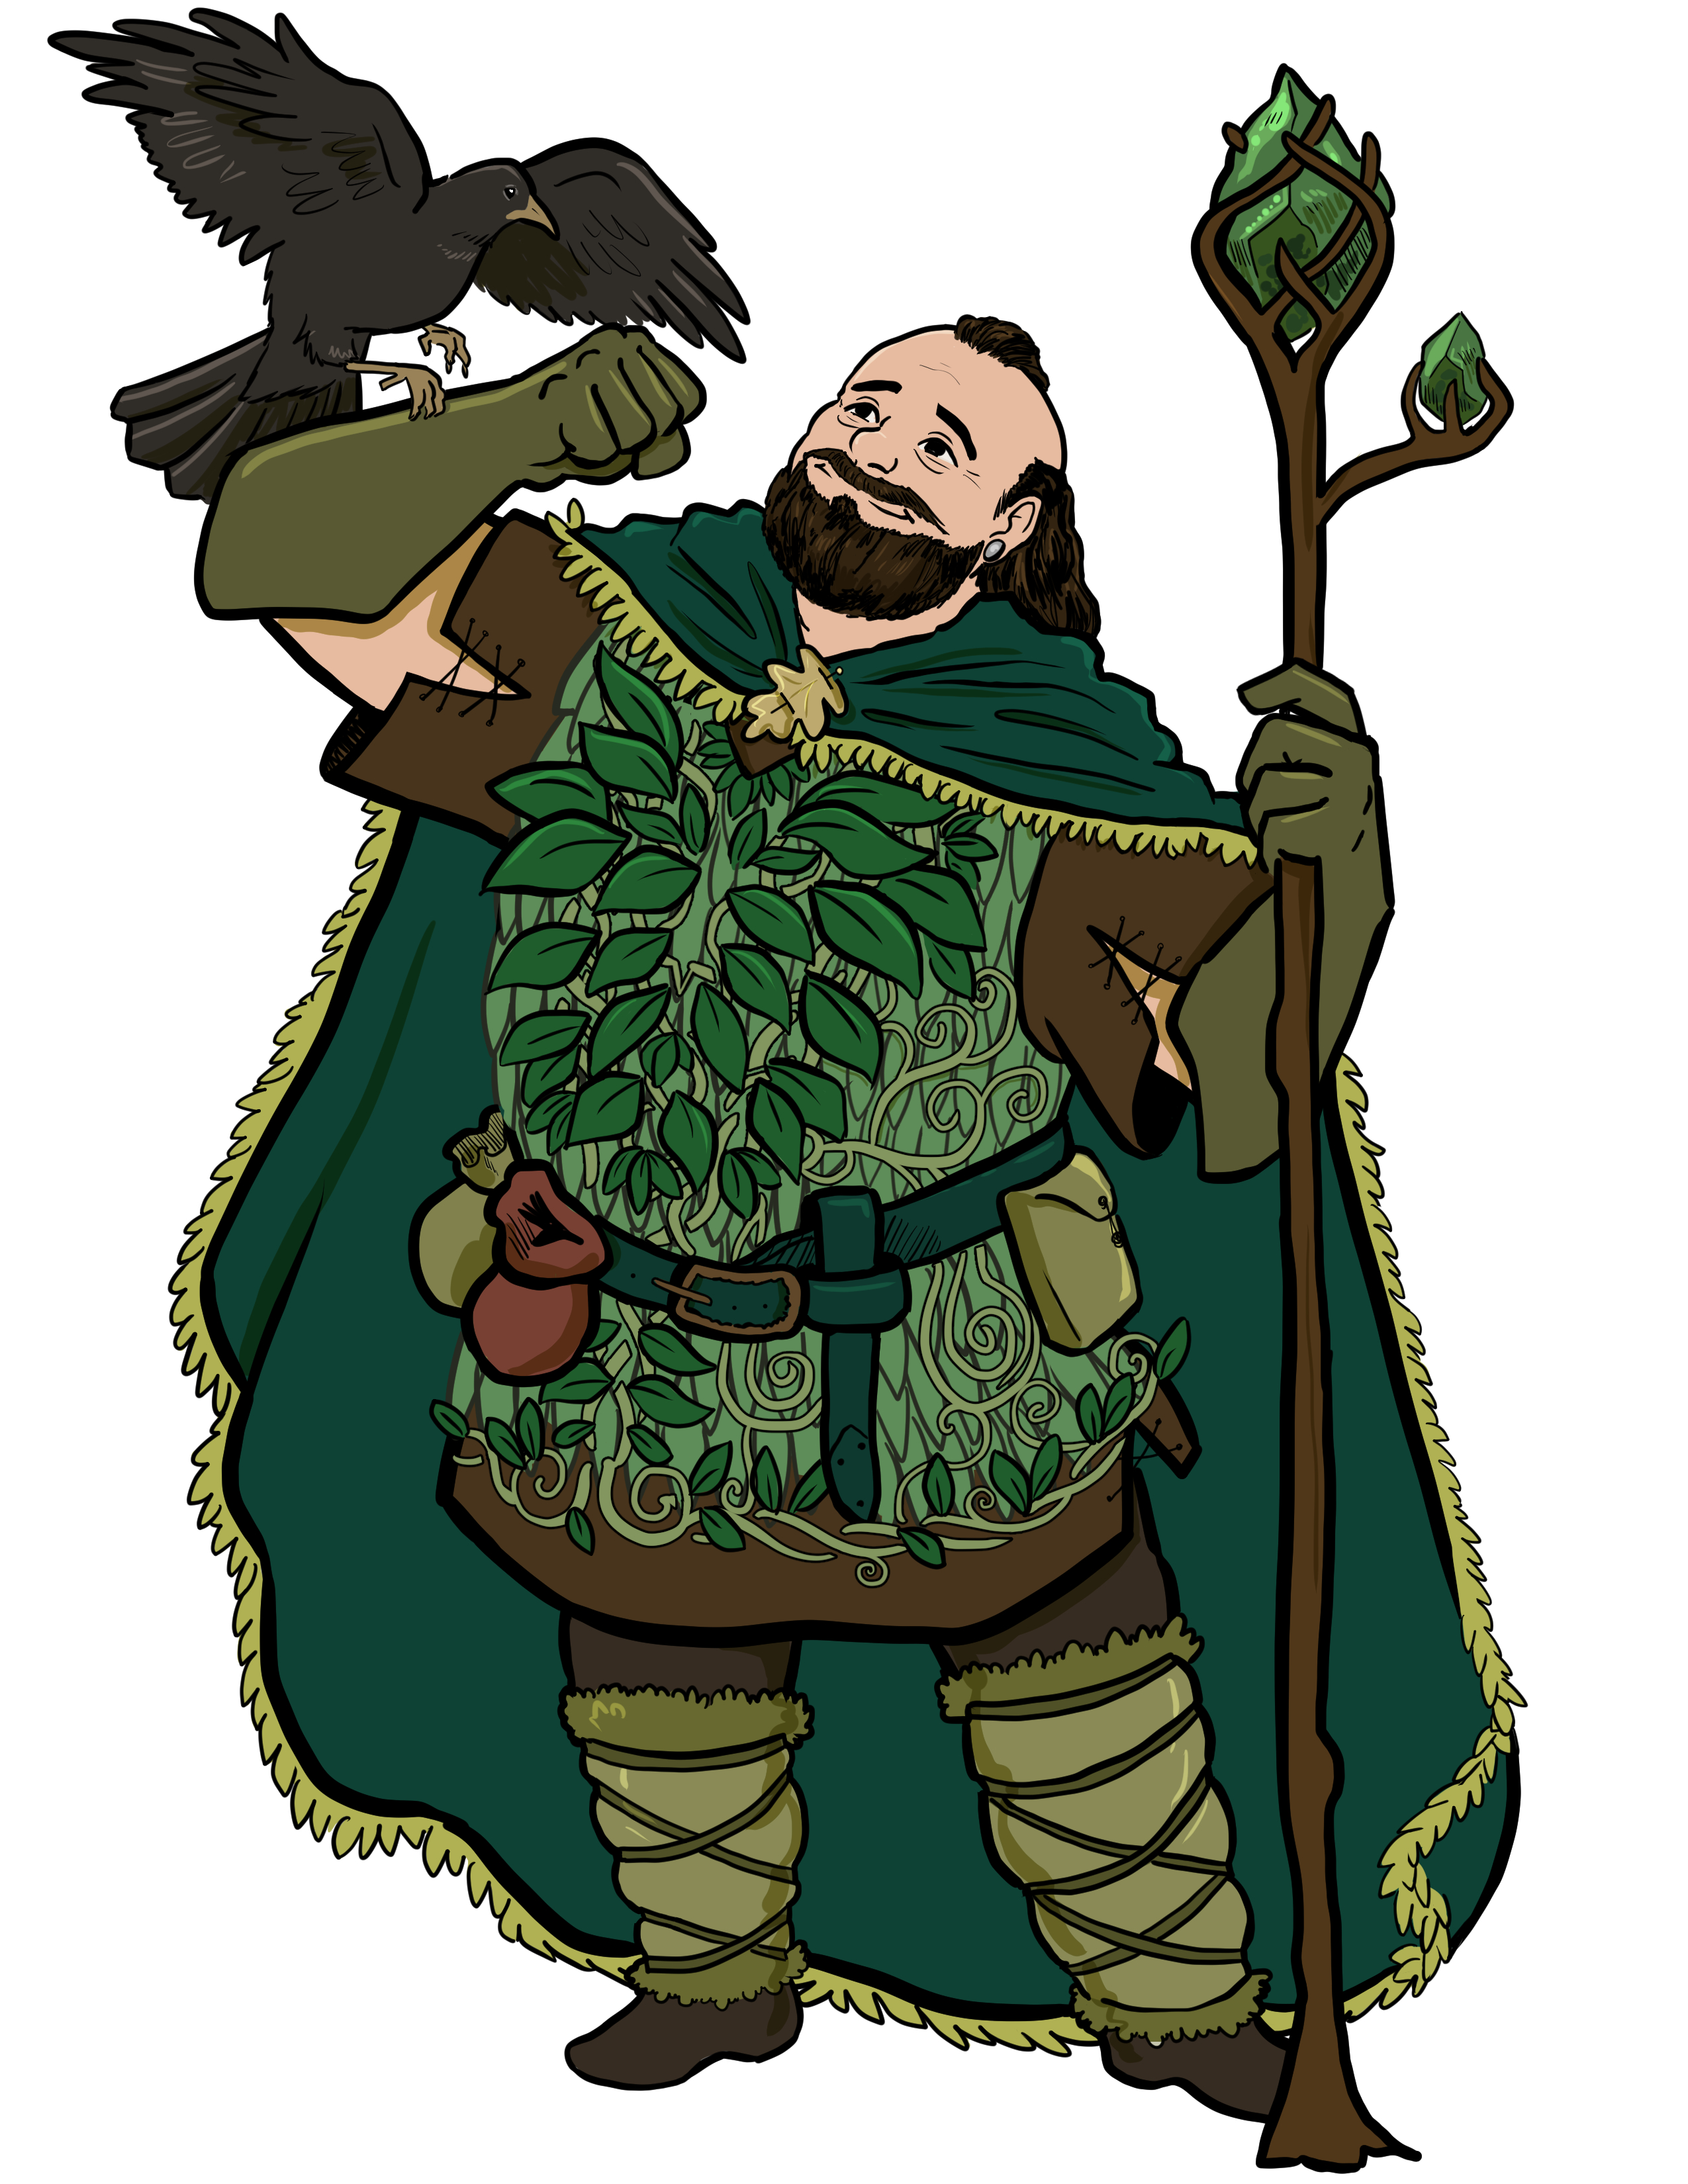
\includegraphics[width=\columnwidth]{Classes/Druid}
Druids are humans who worship nature. In exchange for their worship, they gain the ability to cast spells.

Druids sometimes claim that their worship is older than the first \iref[chap:Immortals]{Immortal}, and that the way that clerics get their power from \iref[chap:Immortals]{Immortals} is a lesser imitation of their own abilities.

While it is true that druids can cast all the spells that clerics can and more, and can do so without needing to come to any kind of arrangement with an \iref[chap:Immortals]{Immortal}, the true relationship between clerical worship and druidic worship is not known; and such theories are mere philosophical speculation.

In fact, no-one knows where druids get their power from. A new initiate vows to respect and protect “Nature”, and when druids commune they do so with “Nature” - and get responses; but if there is any sapient entity personifying nature then it has never revealed itself to either mortal or \iref[chap:Immortals]{Immortal}.

Druidic society has no hierarchy or structure and each druid is effectively their own master, doing as they think right.

The druidic philosophy is primarily concerned with protecting nature from corruption and destruction. As such, druids live apart from civilization, often in woodland areas but occasionally in mountains or desert regions.

Although there are occasional extremists who seek to kill or drive off all those who intrude on their protected areas, most druids are pragmatic in their protection. They will not hinder those who travel through or even hunt in their realms—providing such travel or hunting is done responsibly.

However, they do oppose the encroachment of farmland and cities into their realm, as well as protecting it from unnatural creatures. Druids shun technology, and do not like to use manufactured items. Most will use money on occasion, but will generally prefer to barter for what few goods they use and for their services.

In general, druids will keep on friendly terms with people who live around (or even in) their lands; helping and protecting them in exchange for their keeping respectful of nature.

Within an adventuring party, druids tend to operate in a support role. Their spells emphasize healing and protection rather than flashy attacks.

\subsection{Abilities}
\textbf{Spells:} Starting at \nth{2} level, druids can cast druidic spells. See \fullref{chap:Spells and Spellcasting} for detailed descriptions of these spells.

Providing a druid has had a good night’s sleep (8 hours), they can spend an hour communing with nature after waking up in order to gain spells for the day as indicated on \fullref{tab:Druid Spells per Day by Spell Level}.

Every druid has access to all druid spells of levels they can cast, and chooses freely which ones to prepare each day within the limits of the numbers shown on \fullref{tab:Druid Spells per Day by Spell Level}.

Each prepared spell can be cast once during the day, and if a druid wishes to cast a spell more than once then they must prepare the spell more than once, taking up multiple spell slots of the spell’s level.

Some druidic spells are reversible. These spells can be reversed in order to have an effect opposite to the normal effect of the spell. A druid chooses whether or not to reverse the spell at the time of casting, not at the time of preparation. Druidic spells are always prepared in their normal form.

See \fullref{chap:Spells and Spellcasting} for more information on spells and spellcasting.

\textbf{Charm Plants:} At \nth{10} level, a druid gains the ability to charm plants. This ability functions identically to the \nth{7} level wizard spell \iref[spell:Charm Plant]{Charm Plant}.

\textbf{Immunity to Poisons:} At \nth{10} level, a druid become immune to all poisons.

\textbf{Scry:} At \nth{20} level, a druid can use a small body of water (such as a puddle or a water-filled cauldron) to see any place or object that they desire. A current image of that place or object will appear and last for 10 minutes. The clarity of the image will be based on the familiarity that the druid has with the object or area.

\textbf{Shapechange:} At \nth{30} level, a druid gains the ability to shapechange at will into any non-magical animal. Any equipment worn disappears while in animal form and reappears when returning to human form.

\statblock{\textbf{Ability Requirements:} Wisdom 9

\textbf{Prime Requisite:} Wisdom

\textbf{Hit Dice:} 1d6

\textbf{Movement:} 40 feet

\textbf{Weapons:} Any non-metal blunt

\textbf{Armor:} Hide Armor, Leather Armor, Any non-metal shield

\textbf{Special Abilities:} Spells, Charm Plants, Immunity to Poisons, Scry, Shapechange

\textbf{Required Skills:} First Aid, Nature Lore, Snares, Tracking}

\end{multicols*}
\begin {table}[H]
  \caption{Druid Progression}
	\begin{tabularx}{\columnwidth}{>{\bfseries}cccM{.31in}M{.51in}M{.25in}M{.43in}M{.32in}M{.45in}Y}
    \thead{}&\thead{}&\thead{}&\thead{}&\multicolumn{5}{c}{\thead{Saving Throws}}\thead{}&\setcounter{rownum}{0}\\
    \thead{Level} & \thead{Experience} & \thead{Hit Dice} & \thead{Attack Bonus} & \thead{Death Ray/ Poison} & \thead{Magic Wands} & \thead{Paralysis/ Petrify} & \thead{Breath Weapon} & \thead{Rod/Staff/ Spell} & \thead{Special}\\
		1 & 0 & 1d6 & +1 & 11 & 12 & 14 & 16 & 15 & +4 Skill Points, +2 Weapon Feats\\
		2 & 1,500 & 2d6 & +1 & 11 & 12 & 14 & 16 & 15 & Spells\\
		3 & 3,000 & 3d6 & +1 & 11 & 12 & 14 & 16 & 15 & +1 Weapon Feat\\
		4 & 6,000 & 4d6 & +2 & 10 & 11 & 13 & 15 & 14 & -\\
		5 & 12,000 & 5d6 & +2 & 10 & 11 & 13 & 15 & 14 & +1 Skill Point\\
		6 & 25,000 & 6d6 & +3 & 9 & 10 & 12 & 14 & 13 & +1 Weapon Feat\\
		7 & 50,000 & 7d6 & +3 & 9 & 10 & 12 & 14 & 13 & -\\
		8 & 100,000 & 8d6 & +4 & 8 & 9 & 11 & 13 & 12 & -\\
		9 & 200,000 & 9d6 & +4 & 8 & 9 & 11 & 13 & 12 & +1 Skill Point, +1 Weapon Feat\\
		10 & 300,000 & 9d6+1 & +5 & 7 & 8 & 10 & 12 & 11 & Charm Plants, Immunity to Poisons\\
		11 & 400,000 & 9d6+2 & +5 & 7 & 8 & 10 & 12 & 11 & +1 Weapon Feat\\
		12 & 500,000 & 9d6+3 & +6 & 7 & 8 & 9 & 11 & 10 & -\\
		13 & 600,000 & 9d6+4 & +6 & 6 & 7 & 9 & 11 & 10 & +1 Skill Point\\
		14 & 700,000 & 9d6+5 & +7 & 6 & 7 & 8 & 10 & 9 & -\\
		15 & 800,000 & 9d6+6 & +7 & 6 & 7 & 8 & 10 & 9 & +1 Weapon Feat\\
		16 & 900,000 & 9d6+7 & +8 & 6 & 7 & 7 & 9 & 8 & -\\
		17 & 1,000,000 & 9d6+8 & +8 & 5 & 7 & 7 & 9 & 8 & +1 Skill Point\\
		18 & 1,100,000 & 9d6+9 & +9 & 5 & 7 & 6 & 8 & 7 & -\\
		19 & 1,200,000 & 9d6+10 & +9 & 5 & 7 & 6 & 8 & 7 & -\\
		20 & 1,300,000 & 9d6+11 & +10 & 5 & 6 & 6 & 7 & 6 & Scry\\
		21 & 1,400,000 & 9d6+12 & +10 & 4 & 6 & 5 & 7 & 6 & +1 Skill Point\\
		22 & 1,500,000 & 9d6+13 & +11 & 4 & 5 & 5 & 6 & 5 & -\\
		23 & 1,600,000 & 9d6+14 & +11 & 4 & 5 & 5 & 6 & 5 & +1 Weapon Feat\\
		24 & 1,700,000 & 9d6+15 & +12 & 4 & 5 & 5 & 5 & 5 & -\\
		25 & 1,800,000 & 9d6+16 & +12 & 3 & 4 & 4 & 5 & 4 & +1 Skill Point\\
		26 & 1,900,000 & 9d6+17 & +13 & 3 & 4 & 4 & 4 & 4 & -\\
		27 & 2,000,000 & 9d6+18 & +13 & 3 & 4 & 4 & 4 & 4 & -\\
		28 & 2,100,000 & 9d6+19 & +14 & 3 & 4 & 4 & 4 & 4 & -\\
		29 & 2,200,000 & 9d6+20 & +14 & 2 & 3 & 3 & 3 & 3 & +1 Skill Point\\
		30 & 2,300,000 & 9d6+21 & +15 & 2 & 3 & 3 & 3 & 3 & Shapechange, +1 Weapon Feat\\
		31 & 2,400,000 & 9d6+22 & +15 & 2 & 3 & 3 & 3 & 3 & -\\
		32 & 2,500,000 & 9d6+23 & +16 & 2 & 3 & 3 & 3 & 3 & -\\
		33 & 2,600,000 & 9d6+24 & +16 & 2 & 2 & 2 & 2 & 2 & +1 Skill Point\\
		34 & 2,700,000 & 9d6+25 & +17 & 2 & 2 & 2 & 2 & 2 & -\\
		35 & 2,800,000 & 9d6+26 & +17 & 2 & 2 & 2 & 2 & 2 & -\\
		36 & 2,900,000 & 9d6+27 & +18 & 2 & 2 & 2 & 2 & 2 & +1 Weapon Feat\
  \end {tabularx}
\end {table}
\newpage
\begin{multicols*}{2}

\begin {table}[H]
	\caption{Druid Spells per Day by Spell Level}\label{tab:Druid Spells per Day by Spell Level}
	\begin{tabularx}{\columnwidth}{>{\bfseries}YYYYYYYY}
		\thead{} & \thead{} & \multicolumn{6}{c}{\thead{Spell Level}}\\
		\thead{Level} & \thead{1} & \thead{2} & \thead{3} & \thead{4} & \thead{5} & \thead{6} & \thead{7}\\
		1 & - & - & - & - & - & - & -\\
		2 & 1 & - & - & - & - & - & -\\
		3 & 2 & - & - & - & - & - & -\\
		4 & 2 & 1 & - & - & - & - & -\\
		5 & 2 & 2 & - & - & - & - & -\\
		6 & 2 & 2 & 1 & - & - & - & -\\
		7 & 3 & 2 & 2 & - & - & - & -\\
		8 & 3 & 3 & 2 & 1 & - & - & -\\
		9 & 3 & 3 & 3 & 2 & - & - & -\\
		10 & 4 & 4 & 3 & 2 & 1 & - & -\\
		11 & 4 & 4 & 3 & 3 & 2 & - & -\\
		12 & 4 & 4 & 4 & 3 & 2 & 1 & -\\
		13 & 5 & 5 & 4 & 3 & 2 & 2 & -\\
		14 & 5 & 5 & 5 & 3 & 3 & 2 & -\\
		15 & 6 & 5 & 5 & 3 & 3 & 3 & -\\
		16 & 6 & 5 & 5 & 4 & 4 & 3 & -\\
		17 & 6 & 6 & 5 & 4 & 4 & 3 & 1\\
		18 & 6 & 6 & 5 & 4 & 4 & 3 & 2\\
		19 & 7 & 6 & 5 & 4 & 4 & 4 & 2\\
		20 & 7 & 6 & 5 & 4 & 4 & 4 & 3\\
		21 & 7 & 6 & 5 & 5 & 5 & 4 & 3\\
		22 & 7 & 6 & 5 & 5 & 5 & 4 & 4\\
		23 & 7 & 7 & 6 & 6 & 5 & 4 & 4\\
		24 & 8 & 7 & 6 & 6 & 5 & 5 & 4\\
		25 & 8 & 7 & 6 & 6 & 5 & 5 & 5\\
		26 & 8 & 7 & 7 & 6 & 6 & 5 & 5\\
		27 & 8 & 8 & 7 & 6 & 6 & 6 & 5\\
		28 & 8 & 8 & 7 & 7 & 7 & 6 & 5\\
		29 & 8 & 8 & 7 & 7 & 7 & 6 & 6\\
		30 & 8 & 8 & 8 & 7 & 7 & 7 & 6\\
		31 & 8 & 8 & 8 & 8 & 8 & 7 & 6\\
		32 & 9 & 8 & 8 & 8 & 8 & 7 & 7\\
		33 & 9 & 9 & 8 & 8 & 8 & 8 & 7\\
		34 & 9 & 9 & 9 & 8 & 8 & 8 & 8\\
		35 & 9 & 9 & 9 & 9 & 9 & 8 & 8\\
		36 & 9 & 9 & 9 & 9 & 9 & 9 & 9\
  \end {tabularx}
\end {table}

\section{Dwarf}\index[classes]{Dwarf}\label{class:Dwarf}
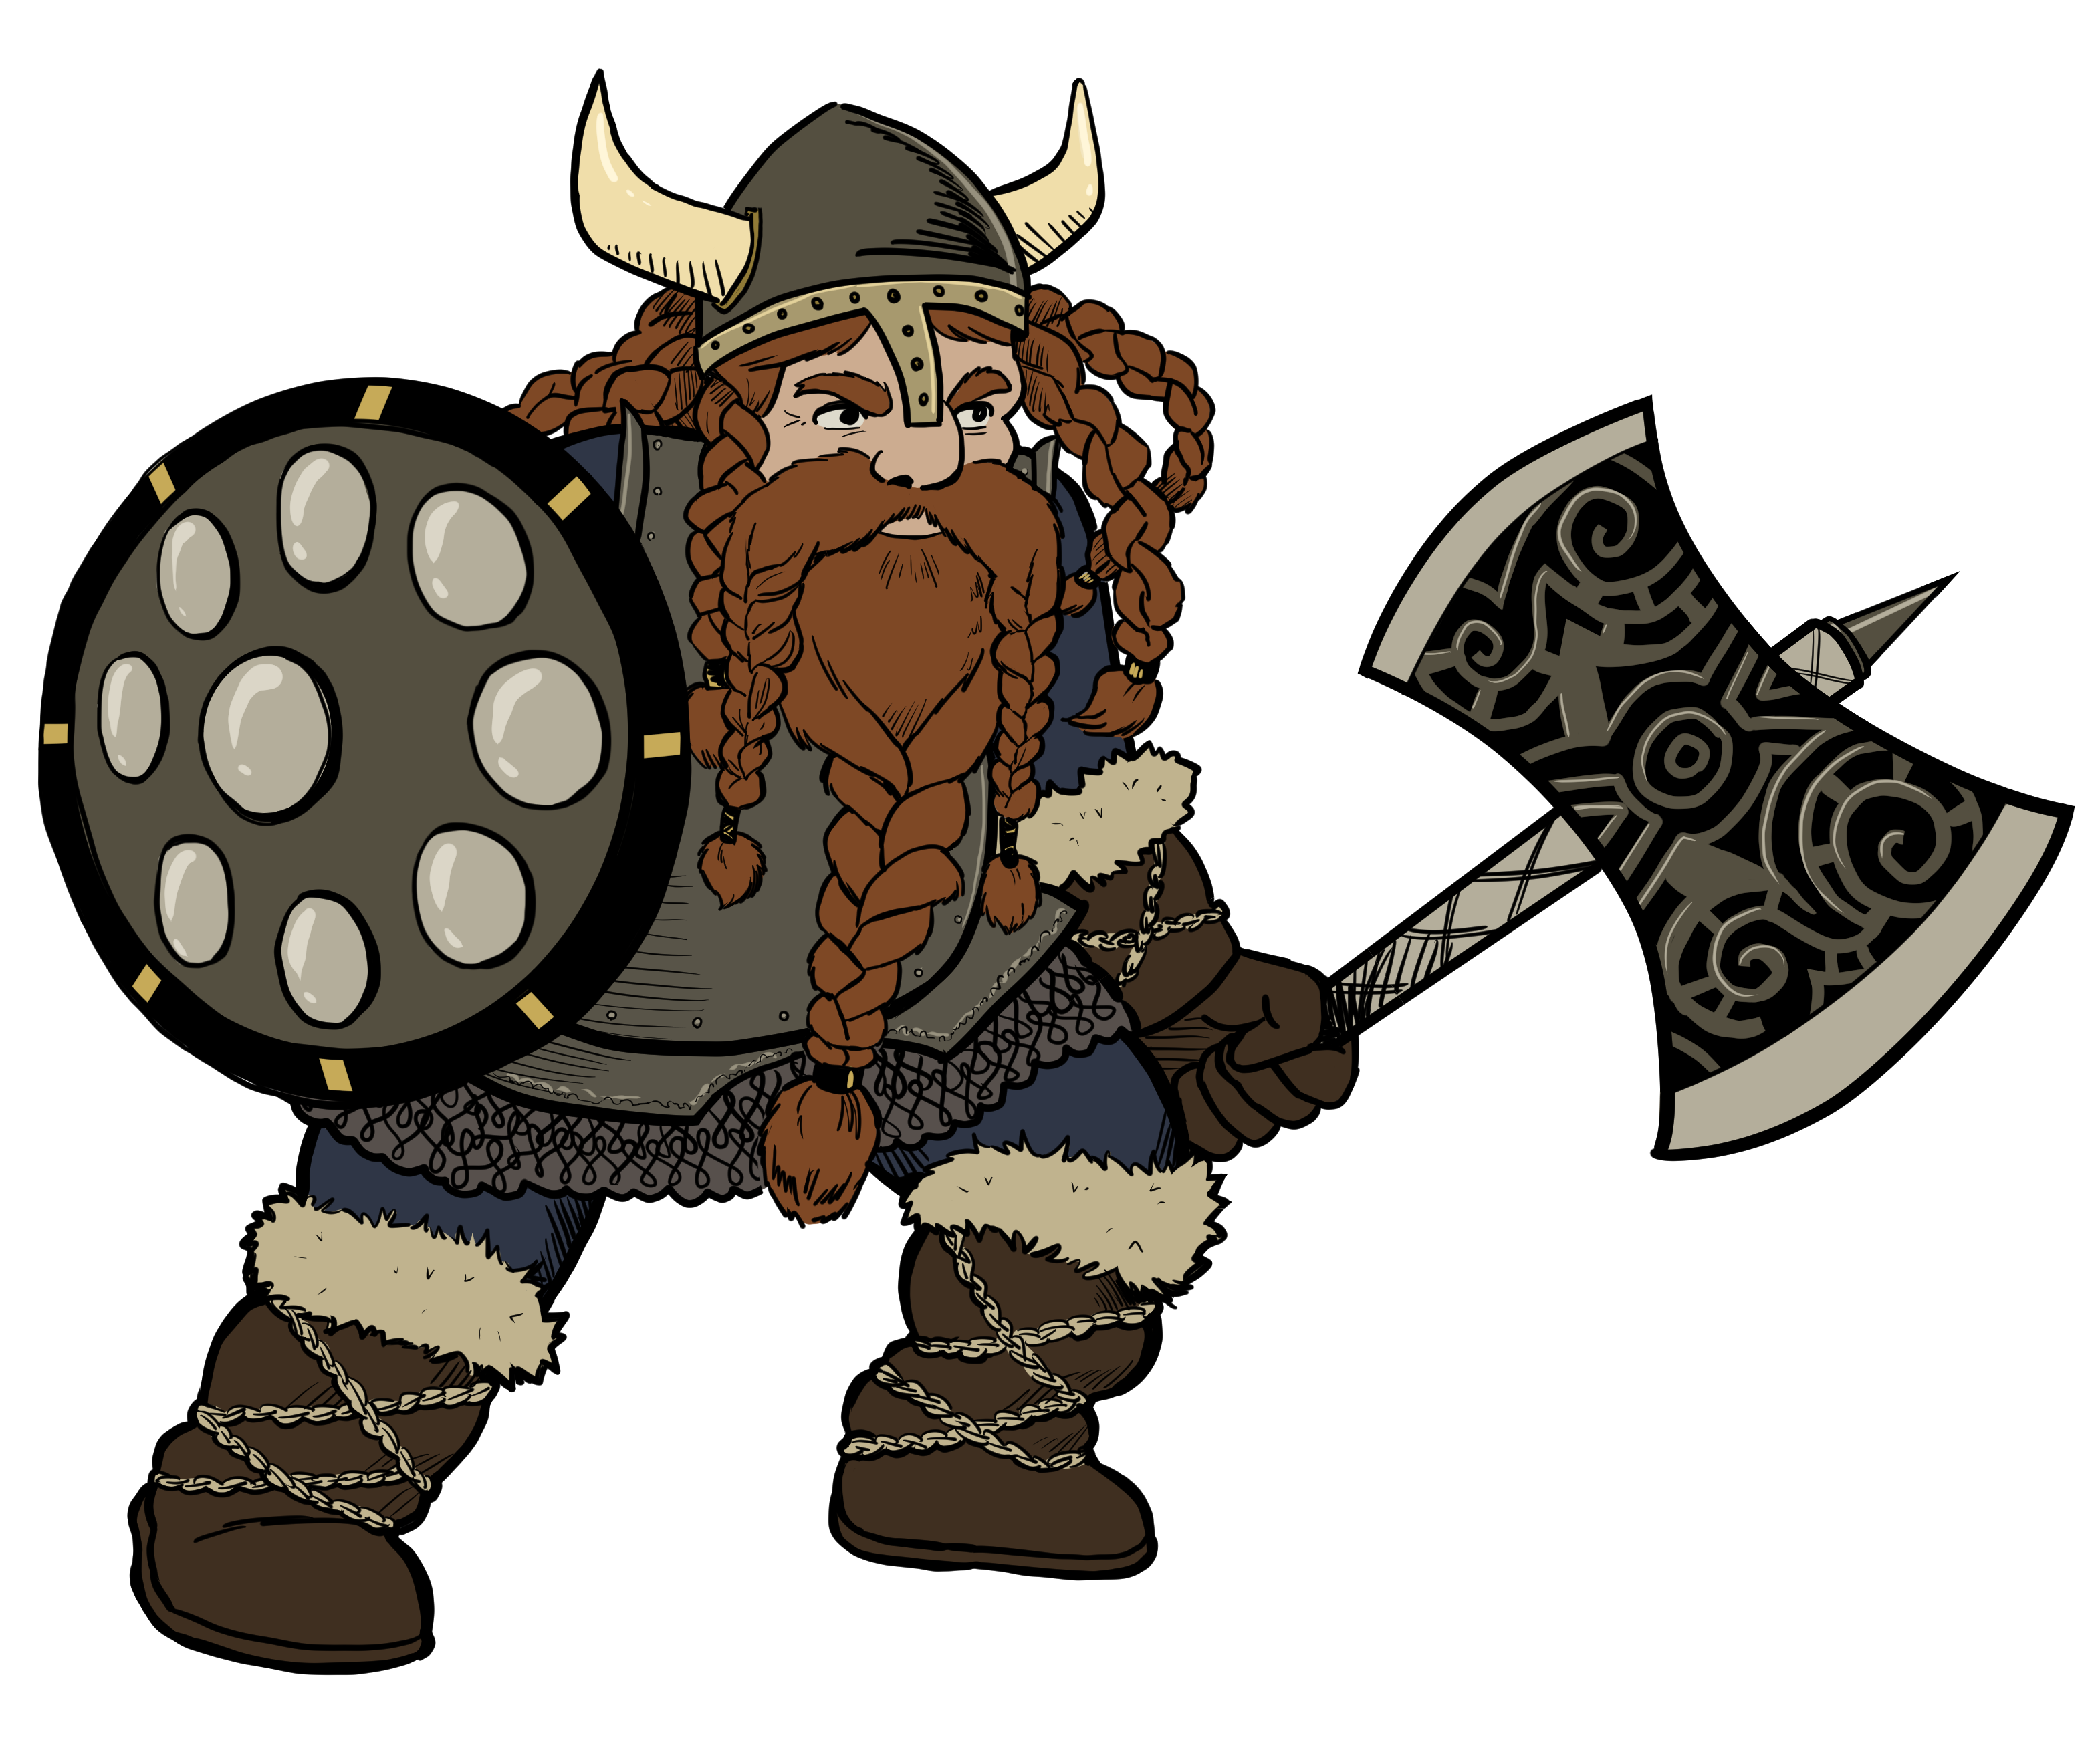
\includegraphics[width=\columnwidth]{Classes/Dwarf}
Dwarves are a demi-human race. Like most demi-human races, they are less flexible than humans, and all dwarf adventurers are represented by a single class.

Physically, dwarves are slightly shorter than humans but are similar in weight due to their stockier build. Skin and hair color shows the same range as humans, although both male and female dwarves tend to have slightly more facial and body hair than humans and both sexes usually sport beards.

Traditionally, dwarves live in mountainous areas near humans, where they live underground and use their mining and metal-working skills to make goods and tools that they can trade with the humans for food and textiles.

Dwarves are an inherently non-magical race, and possess no magic users or clerics of their own—not even being able to produce the lesser shamans that goblins and giants—their traditional enemies—are able to field in battle. However, this lack of magical ability makes dwarves much more resilient and able to resist magical attacks.

Dwarven adventurers make tough warriors who are at home in underground environments.

\subsection{Abilities}
\textbf{Infravision:} Dwarves have \iref[sec:Infravision]{Infravision} (see \fullref{sec:Infravision}).

\textbf{Stonelore:}\label{sec:Stonelore} A dwarf’s experience with masonry and stonework—in particular underground stonework—gives them a chance to detect irregularities in construction. If a dwarf examines an area looking for irregularities, the Game Master should secretly roll 1d6 for each feature in the area being searched that is one of the following:

\begin{itemize}
	\item{Traps involving moving stone walls or blocks of stone}
	\item{Secret doors involving moving stone walls.}
	\item{Newly built stone constructions.}
	\item{Gently sloping stonework.}
\end{itemize}

In each case, if the 1d6 roll is a 1-2, the dwarf is able to detect the feature. If the roll is a 3-6, then the dwarf in unable to detect the feature (and the dwarf’s player should not be told whether this was because the roll failed or because there was no feature to detect).

\textbf{Fighter Abilities:} At \nth{12} level and higher, a dwarf can use the following fighter abilities: Parry and Smash, and Multiple Attacks (at \nth{12}, \nth{20}, and \nth{36} level).

\textbf{Spell Resistance:} At \nth{16} level and higher, a dwarf only takes half damage from all spells and spell-like abilities. If the attack normally allows a saving throw for half damage then the dwarf only takes a quarter of normal damage if they save successfully.

\statblock{\textbf{Ability Requirements:} Constitution 9

\textbf{Prime Requisite:} Strength

\textbf{Ability Modifiers:} Constitution +1, Charisma -1

\textbf{Hit Dice:} 1d8

\textbf{Movement:} 20 feet

\textbf{Weapons:} Any except large

\textbf{Armor:} Any except large shields

\textbf{Special Abilities:} Infravision, Stonelore, Multiple Attacks, Parry, Smash, Spell Resistance}

\end{multicols*}
\begin {table}[H]
  \caption{Dwarf Progression}
	\begin{tabularx}{\columnwidth}{>{\bfseries}cccM{.31in}M{.51in}M{.25in}M{.43in}M{.32in}M{.45in}Y}
    \thead{}&\thead{}&\thead{}&\thead{}&\multicolumn{5}{c}{\thead{Saving Throws}}\thead{}&\setcounter{rownum}{0}\\
    \thead{Level} & \thead{Experience} & \thead{Hit Dice} & \thead{Attack Bonus} & \thead{Death Ray/ Poison} & \thead{Magic Wands} & \thead{Paralysis/ Petrify} & \thead{Breath Weapon} & \thead{Rod/Staff/ Spell} & \thead{Special}\\
		1 & 0 & 1d8 & +1 & 8 & 9 & 10 & 13 & 12 & Infravision, Stonelore, +4 Skill Points, +4 Weapon Feats\\
		2 & 2,200 & 2d8 & +1 & 8 & 9 & 10 & 13 & 12 & -\\
		3 & 4,400 & 3d8 & +2 & 7 & 8 & 9 & 12 & 11 & +1 Weapon Feat\\
		4 & 8,800 & 4d8 & +2 & 7 & 8 & 9 & 11 & 10 & -\\
		5 & 17,000 & 5d8 & +3 & 6 & 7 & 8 & 10 & 9 & +1 Skill Point\\
		6 & 35,000 & 6d8 & +4 & 5 & 6 & 7 & 9 & 8 & +1 Weapon Feat\\
		7 & 70,000 & 7d8 & +4 & 5 & 6 & 7 & 8 & 7 & -\\
		8 & 140,000 & 8d8 & +5 & 4 & 5 & 6 & 7 & 6 & -\\
		9 & 270,000 & 9d8 & +6 & 3 & 4 & 5 & 6 & 5 & +1 Skill Point, +1 Weapon Feat\\
		10 & 400,000 & 9d8+2 & +6 & 3 & 4 & 5 & 5 & 4 & -\\
		11 & 530,000 & 9d8+4 & +7 & 2 & 3 & 4 & 4 & 3 & +1 Weapon Feat\\
		12 & 660,000 & 9d8+6 & +8 & 2 & 3 & 4 & 4 & 3 & Multiple Attacks, Parry, Smash\\
		13 & 800,000 & 9d8+8 & +8 & 2 & 3 & 4 & 3 & 3 & +1 Skill Point\\
		14 & 1,000,000 & 9d8+10 & +9 & 2 & 3 & 4 & 3 & 3 & -\\
		15 & 1,200,000 & 9d8+12 & +10 & 2 & 2 & 3 & 2 & 2 & +1 Weapon Feat\\
		16 & 1,400,000 & 9d8+14 & +10 & 2 & 2 & 3 & 2 & 2 & Spell Resistance\\
		17 & 1,600,000 & 9d8+16 & +11 & 2 & 2 & 3 & 2 & 2 & +1 Skill Point\\
		18 & 1,800,000 & 9d8+18 & +12 & 2 & 2 & 3 & 2 & 2 & -\\
		19 & 2,000,000 & 9d8+20 & +12 & 2 & 2 & 2 & 2 & 2 & +1 Weapon Feat\\
		20 & 2,200,000 & 9d8+22 & +13 & 2 & 2 & 2 & 2 & 2 & Multiple Attacks (3)\\
		21 & 2,400,000 & 9d8+24 & +14 & 2 & 2 & 2 & 2 & 2 & +1 Skill Point\\
		22 & 2,600,000 & 9d8+26 & +14 & 2 & 2 & 2 & 2 & 2 & -\\
		23 & 2,800,000 & 9d8+28 & +15 & 2 & 2 & 2 & 2 & 2 & +1 Weapon Feat\\
		24 & 3,000,000 & 9d8+30 & +16 & 2 & 2 & 2 & 2 & 2 & -\\
		25 & 3,200,000 & 9d8+32 & +16 & 2 & 2 & 2 & 2 & 2 & +1 Skill Point\\
		26 & 3,400,000 & 9d8+34 & +17 & 2 & 2 & 2 & 2 & 2 & -\\
		27 & 3,600,000 & 9d8+36 & +18 & 2 & 2 & 2 & 2 & 2 & +1 Weapon Feat\\
		28 & 3,800,000 & 9d8+38 & +18 & 2 & 2 & 2 & 2 & 2 & -\\
		29 & 4,000,000 & 9d8+40 & +19 & 2 & 2 & 2 & 2 & 2 & +1 Skill Point\\
		30 & 4,200,000 & 9d8+42 & +20 & 2 & 2 & 2 & 2 & 2 & +1 Weapon Feat\\
		31 & 4,400,000 & 9d8+44 & +20 & 2 & 2 & 2 & 2 & 2 & -\\
		32 & 4,600,000 & 9d8+46 & +21 & 2 & 2 & 2 & 2 & 2 & -\\
		33 & 4,800,000 & 9d8+48 & +22 & 2 & 2 & 2 & 2 & 2 & +1 Skill Point, +1 Weapon Feat\\
		34 & 5,000,000 & 9d8+50 & +22 & 2 & 2 & 2 & 2 & 2 & -\\
		35 & 5,200,000 & 9d8+52 & +23 & 2 & 2 & 2 & 2 & 2 & -\\
		36 & 5,400,000 & 9d8+54 & +23 & 2 & 2 & 2 & 2 & 2 & Multiple Attacks (4), +1 Weapon Feat\
  \end {tabularx}
\end {table}
\newpage
\begin{multicols*}{2}

\section{Elf}\index[classes]{Elf}\label{class:Elf}
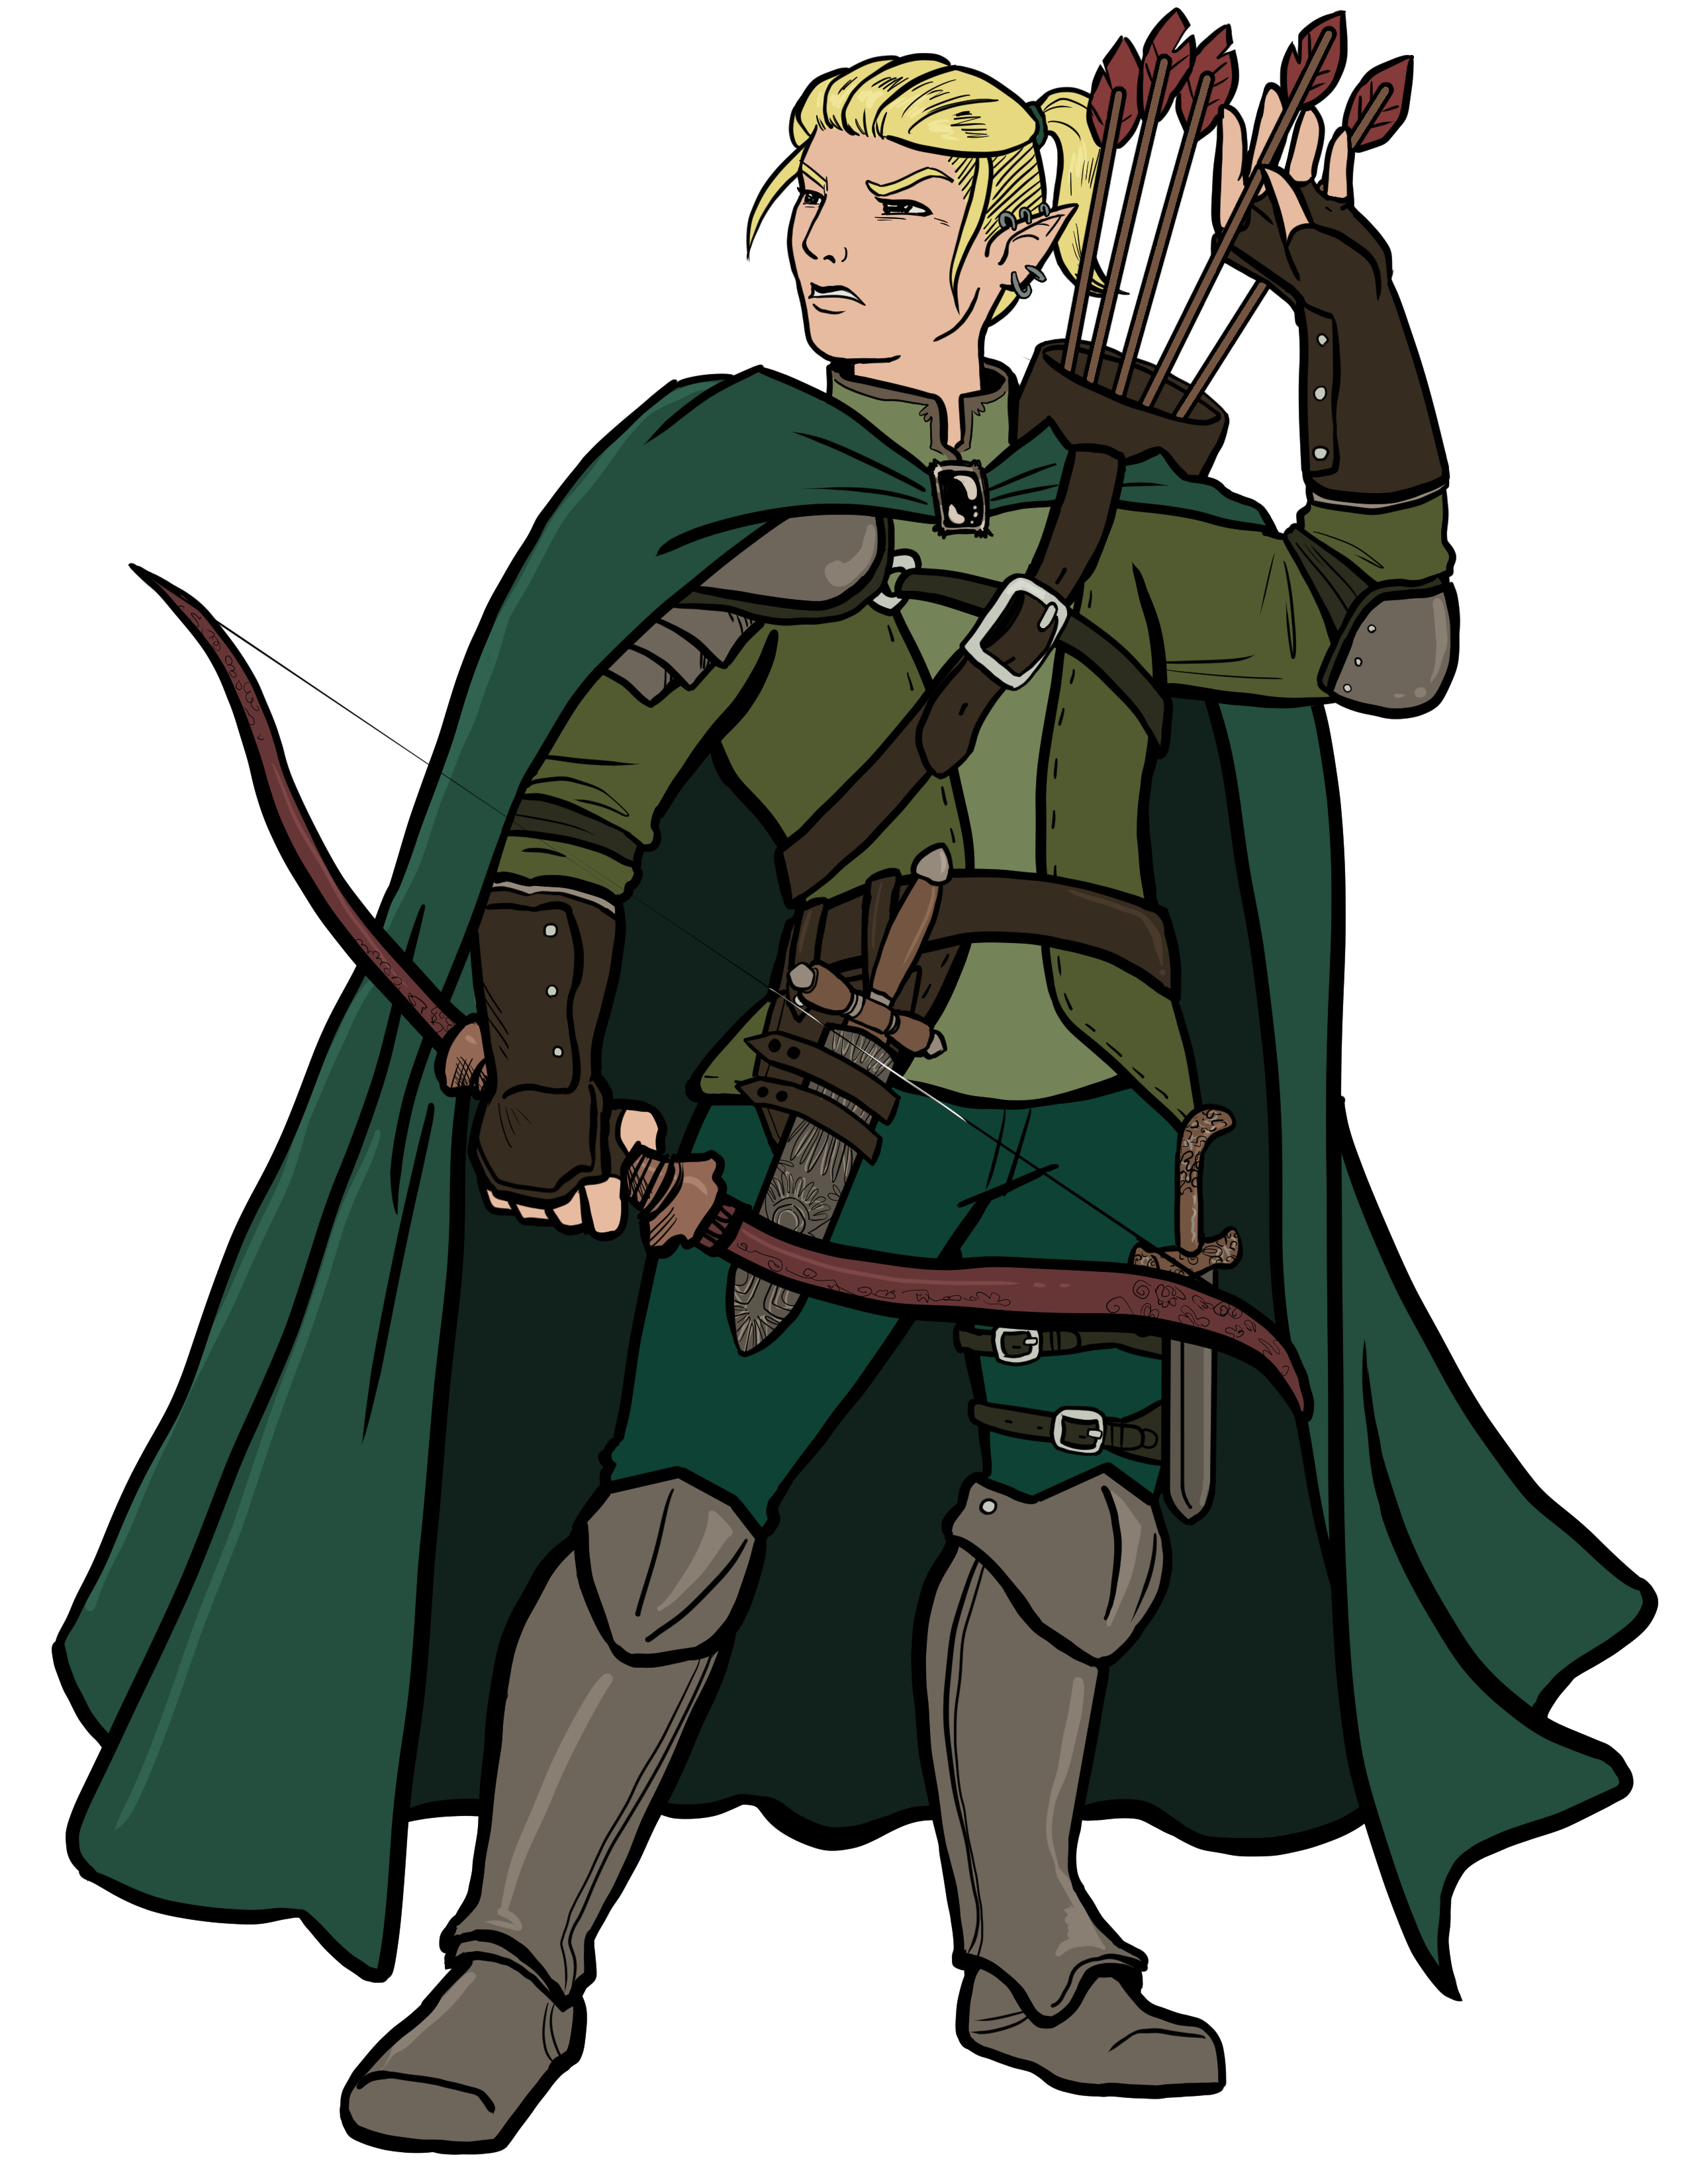
\includegraphics[width=\columnwidth]{Classes/Elf}
Elves are a demi-human race. Like most demi-human races, they are less flexible than humans, and all elf adventurers are represented by a single class.

Elves are more slender and graceful than humans, but they are approximately the same height. Although elves show a similar range of skin colors to those of humans in terms of shade, the hue of their skin tends to be more yellow-brown than that of humans giving them a coloration resembling that of wood anywhere from light pine through to dark ebony. The ears of elves are pointed.

Elves have no body or facial hair, although the hair on their heads is luxuriant, and changes color throughout their life like the colors of leaves change through seasons—starting a light green and slowly darkening, as the elf matures before changing to brown, gold and red in old age.

Elves are naturally magical creatures, and all elves are capable of casting low level magical spells.

Elven adventurers are usually much more highly skilled and have spellcasting abilities rivaling the finest human magic users. However, despite their inherent magic elves are unable to become clerics or shamans.

Elves usually live in woodland or forest, and have an affinity for trees. Their towns tend to be in the treetops, woven out of living branches. Elven communities usually have a deep respect for nature, and work together with human druids.

Elves are fine crafters of wood, and although they rarely mine for it themselves they are capable of delicate metalwork as well. Their natural magical ability makes them excellent producers of magic items known for their physical beauty as well as their power.

In an adventuring situation, elves can both fight competently (although not quite as well as a human fighter) and use magic making them very flexible. Elven characters pay for this, however, by advancing in level the most slowly of any class.

\subsection{Abilities}
\textbf{Elfsight:} The superior eyesight of elves enables them to find secret and hidden doors (see \fullref{sec:Doors}) more easily than other characters.

\textbf{Ghoul Immunity:} Elves are immune to the paralysis caused by the touch of ghouls and ghasts. They are not immune to other forms of paralysis.

\textbf{Infravision:} Elves have \iref[sec:Infravision]{Infravision} (see \fullref{sec:Infravision}).

\textbf{Spells:} Elves can cast elf spells. See \fullref{chap:Spells and Spellcasting} for detailed descriptions of these spells.

Providing an elf has had a good night’s sleep (8 hours), they can spend an hour studying their spell book after waking up in order to gain spells for the day as indicated on \fullref{tab:Elf Spells per Day by Spell Level}.

A \nth{1} level elf starts with only two spells in their spell book, and must acquire more during their adventures. Elves may prepare any spell from their book in either the normal or the reversed form (if the spell has a reversed form), but may not prepare spells from someone else’s book or from a scroll; not even by using a \iref[spell:Read Magic]{Read Magic} spell.

Each prepared spell can be cast once during the day, and if an elf wishes to cast a spell more than once then they must prepare the spell more than once, taking up multiple spell slots of the spell’s level. Some magic user spells are reversible. These spells can be reversed in order to have an effect opposite to the normal effect of the spell. An elf chooses whether or not to reverse the spell at the time of preparation, not at the time of casting.

A beginning elf starts with a spell book given to them by their master, and this spell book will contain the spell Read Magic and one other \nth{1} level spell of the player’s choice. This spell book is a gift from the character’s master and does not need to be paid for.

See \fullref{chap:Spells and Spellcasting} for more information on spells and spellcasting.

\textbf{Fighter Abilities:} At \nth{11} level and higher, an elf can use the following fighter abilities: Parry and Smash, and Multiple Attacks (at \nth{11} and \nth{18} level).

\textbf{Breath Evasion:} At \nth{14} level and higher, an elf only takes half damage from all breath weapons such as those used by dragons. If the attack normally allows a saving throw for half damage then the elf only takes a quarter of normal damage if they save successfully.

\statblock{\textbf{Ability Requirements:} Intelligence 9

\textbf{Prime Requisite:} Strength and Intelligence

\textbf{Ability Modifiers:} Dexterity +1, Constitution -1

\textbf{Hit Dice:} 1d6

\textbf{Movement:} 40 feet

\textbf{Weapons:} Any

\textbf{Armor:} Any

\textbf{Special Abilities:} Elfsight, Ghoul Immunity, Infravision, Spells, Multiple Attacks, Parry, Smash, Breath Evasion}

\end{multicols*}
\begin {table}[H]
  \caption{Elf Progression}
	\begin{tabularx}{\columnwidth}{>{\bfseries}cccM{.31in}M{.51in}M{.25in}M{.43in}M{.32in}M{.45in}Y}
    \thead{}&\thead{}&\thead{}&\thead{}&\multicolumn{5}{c}{\thead{Saving Throws}}\thead{}&\setcounter{rownum}{0}\\
    \thead{Level} & \thead{Experience} & \thead{Hit Dice} & \thead{Attack Bonus} & \thead{Death Ray/ Poison} & \thead{Magic Wands} & \thead{Paralysis/ Petrify} & \thead{Breath Weapon} & \thead{Rod/Staff/ Spell} & \thead{Special}\\
		1 & 0 & 1d6 & +1 & 12 & 13 & 13 & 15 & 15 & Elfsight, Ghoul Immunity, Infravision, 
+4 Skill Points, +2 Weapon Feats\\
		2 & 4,000 & 2d6 & +1 & 12 & 13 & 13 & 15 & 15 & -\\
		3 & 8,000 & 3d6 & +1 & 11 & 12 & 12 & 14 & 14 & +1 Weapon Feat\\
		4 & 16,000 & 4d6 & +2 & 9 & 11 & 11 & 12 & 12 & -\\
		5 & 32,000 & 5d6 & +2 & 8 & 10 & 10 & 11 & 11 & +1 Skill Point\\
		6 & 64,000 & 6d6 & +3 & 7 & 9 & 9 & 10 & 10 & +1 Weapon Feat\\
		7 & 120,000 & 7d6 & +3 & 5 & 8 & 8 & 8 & 8 & -\\
		8 & 250,000 & 8d6 & +4 & 4 & 7 & 7 & 7 & 7 & -\\
		9 & 400,000 & 9d6 & +4 & 3 & 6 & 6 & 6 & 6 & +1 Skill Point, +1 Weapon Feat\\
		10 & 600,000 & 9d6+1 & +5 & 3 & 5 & 5 & 4 & 4 & -\\
		11 & 850,000 & 9d6+2 & +5 & 2 & 4 & 4 & 3 & 3 & Multiple Attacks (2), Smash, Parry, +1 Weapon Feat\\
		12 & 1,100,000 & 9d6+3 & +6 & 2 & 4 & 4 & 3 & 3 & -\\
		13 & 1,350,000 & 9d6+4 & +6 & 2 & 4 & 4 & 2 & 2 & +1 Skill Point\\
		14 & 1,600,000 & 9d6+5 & +7 & 2 & 3 & 3 & 2 & 2 & Breath Evasion\\
		15 & 1,850,000 & 9d6+6 & +7 & 2 & 3 & 3 & 2 & 2 & +1 Weapon Feat\\
		16 & 2,100,000 & 9d6+7 & +8 & 2 & 3 & 3 & 2 & 2 & -\\
		17 & 2,350,000 & 9d6+8 & +8 & 2 & 2 & 2 & 2 & 2 & +1 Skill Point\\
		18 & 2,600,000 & 9d6+9 & +9 & 2 & 2 & 2 & 2 & 2 & Multiple Attacks (3)\\
		19 & 2,850,000 & 9d6+10 & +9 & 2 & 2 & 2 & 2 & 2 & -\\
		20 & 3,100,000 & 9d6+11 & +10 & 2 & 2 & 2 & 2 & 2 & -\\
		21 & 3,300,000 & 9d6+12 & +10 & 2 & 2 & 2 & 2 & 2 & +1 Skill Point\\
		22 & 3,500,000 & 9d6+13 & +11 & 2 & 2 & 2 & 2 & 2 & -\\
		23 & 3,700,000 & 9d6+14 & +11 & 2 & 2 & 2 & 2 & 2 & +1 Weapon Feat\\
		24 & 3,900,000 & 9d6+15 & +12 & 2 & 2 & 2 & 2 & 2 & -\\
		25 & 4,100,000 & 9d6+16 & +12 & 2 & 2 & 2 & 2 & 2 & +1 Skill Point\\
		26 & 4,300,000 & 9d6+17 & +13 & 2 & 2 & 2 & 2 & 2 & -\\
		27 & 4,500,000 & 9d6+18 & +13 & 2 & 2 & 2 & 2 & 2 & -\\
		28 & 4,700,000 & 9d6+19 & +14 & 2 & 2 & 2 & 2 & 2 & -\\
		29 & 4,900,000 & 9d6+20 & +14 & 2 & 2 & 2 & 2 & 2 & +1 Skill Point\\
		30 & 5,100,000 & 9d6+21 & +15 & 2 & 2 & 2 & 2 & 2 & +1 Weapon Feat\\
		31 & 5,300,000 & 9d6+22 & +15 & 2 & 2 & 2 & 2 & 2 & -\\
		32 & 5,500,000 & 9d6+23 & +16 & 2 & 2 & 2 & 2 & 2 & -\\
		33 & 5,700,000 & 9d6+24 & +16 & 2 & 2 & 2 & 2 & 2 & +1 Skill Point\\
		34 & 5,900,000 & 9d6+25 & +17 & 2 & 2 & 2 & 2 & 2 & -\\
		35 & 6,100,000 & 9d6+26 & +17 & 2 & 2 & 2 & 2 & 2 & -\\
		36 & 6,300,000 & 9d6+27 & +18 & 2 & 2 & 2 & 2 & 2 & +1 Weapon Feat\
  \end {tabularx}
\end {table}
\newpage
\begin{multicols*}{2}

\begin {table}[H]
	\caption{Elf Spells per Day by Spell Level}\label{tab:Elf Spells per Day by Spell Level}
  \begin{tabularx}{\columnwidth}{>{\bfseries}YYYYYYYYYY}
		\thead{} & \multicolumn{9}{c}{\thead{Spell Level}}\\
		\thead{Level} & \thead{1} & \thead{2} & \thead{3} & \thead{4} & \thead{5} & \thead{6} & \thead{7} & \thead{8} & \thead{9}\\
		1 & 1 & - & - & - & - & - & - & - & -\\
		2 & 2 & - & - & - & - & - & - & - & -\\
		3 & 2 & 1 & - & - & - & - & - & - & -\\
		4 & 2 & 2 & - & - & - & - & - & - & -\\
		5 & 2 & 2 & 1 & - & - & - & - & - & -\\
		6 & 3 & 2 & 2 & - & - & - & - & - & -\\
		7 & 3 & 2 & 2 & 1 & - & - & - & - & -\\
		8 & 3 & 3 & 2 & 2 & - & - & - & - & -\\
		9 & 3 & 3 & 2 & 2 & 1 & - & - & - & -\\
		10 & 4 & 3 & 3 & 2 & 2 & - & - & - & -\\
		11 & 4 & 4 & 4 & 3 & 2 & - & - & - & -\\
		12 & 4 & 4 & 4 & 3 & 2 & 1 & - & - & -\\
		13 & 5 & 4 & 4 & 3 & 2 & 2 & - & - & -\\
		14 & 5 & 4 & 4 & 4 & 3 & 2 & - & - & -\\
		15 & 5 & 4 & 4 & 4 & 3 & 2 & 1 & - & -\\
		16 & 5 & 5 & 5 & 4 & 3 & 2 & 2 & - & -\\
		17 & 6 & 5 & 5 & 4 & 4 & 3 & 2 & - & -\\
		18 & 6 & 5 & 5 & 4 & 4 & 3 & 2 & 1 & -\\
		19 & 6 & 5 & 5 & 5 & 4 & 3 & 2 & 2 & -\\
		20 & 6 & 5 & 5 & 5 & 4 & 4 & 3 & 2 & -\\
		21 & 6 & 5 & 5 & 5 & 4 & 4 & 3 & 2 & 1\\
		22 & 6 & 6 & 5 & 5 & 5 & 4 & 3 & 2 & 2\\
		23 & 6 & 6 & 6 & 6 & 5 & 4 & 3 & 3 & 2\\
		24 & 7 & 7 & 6 & 6 & 5 & 5 & 4 & 3 & 2\\
		25 & 7 & 7 & 6 & 6 & 5 & 5 & 4 & 4 & 3\\
		26 & 7 & 7 & 7 & 6 & 6 & 5 & 5 & 4 & 3\\
		27 & 7 & 7 & 7 & 6 & 6 & 5 & 5 & 5 & 4\\
		28 & 8 & 8 & 7 & 6 & 6 & 6 & 6 & 5 & 4\\
		29 & 8 & 8 & 7 & 7 & 7 & 6 & 6 & 5 & 5\\
		30 & 8 & 8 & 8 & 7 & 7 & 7 & 6 & 6 & 5\\
		31 & 8 & 8 & 8 & 7 & 7 & 7 & 7 & 6 & 6\\
		32 & 9 & 8 & 8 & 8 & 8 & 7 & 7 & 7 & 6\\
		33 & 9 & 9 & 9 & 8 & 8 & 8 & 7 & 7 & 7\\
		34 & 9 & 9 & 9 & 9 & 8 & 8 & 8 & 8 & 7\\
		35 & 9 & 9 & 9 & 9 & 9 & 9 & 8 & 8 & 8\\
		36 & 9 & 9 & 9 & 9 & 9 & 9 & 9 & 9 & 9\
  \end {tabularx}
\end {table}

\subsection{Subclasses}
\subsubsection{Aquatic Elf}\index[classes]{Aquatic Elf}
Aquatic elves are similar to normal elves, but have gills on their neck and blue or green hair.

Aquatic elves live on the bottom of vast oceans and make their homes in large caverns in lagoon bottoms and reefs.

\textbf{Air/Water Breathing:} Aquatic elves are able to breath both air and water.

\textbf{Dolphin Song:} Aquatic elves can communicate with dolphins and whales within 500 feet by singing their language. They may also use this song to communicate with other aquatic elves.

\textbf{Hide in Reefs/Weeds:} While underwater, an aquatic elf is able to effectively hide in reefs and weeds as long as they remain motionless. The percentage chance of success is 95\%.

Beginning at \nth{2} level, an aquatic elf can move at 1/4 their normal speed while hidden. The percentage chance of success is 10\% per level beyond \nth{1}. The aquatic elf may move half their normal speed by halving their chance of success or 3/4 by quartering it. The maximum chance of success regardless of speed is 95\%.

\statblock{\textbf{Ability Modifiers:} Intelligence +1, Wisdom -1

\textbf{Natural AC:} 7}

\subsubsection{Dark Elf}\index[classes]{Dark Elf}
Dark elves are similar to normal elves, but have white skin and unusually large ears.

Dark elves live in deep underground caverns.

\textbf{Light Sensitivity:} Dark elves' eyes are sensitive to light. While exposed to bright light they suffer a -1 penalty to hit.

\subsubsection{Half-Elf}\index[classes]{Half-Elf}
Half-elves are the offspring of a human and an elf. They are indistinguishable from humans other than their pointed ears. When producing their own offspring (whether their mate is a human or an elf), there is a 65\% chance that the half-elf’s offspring will also be a half-elf.

Half-elves are not a class on their own. The half-elf’s player must choose a human class for them to become. In addition to their chosen class’s abilities, half-elves gain \iref[sec:Infravision]{Infravision} as normal elves, but suffer a 5\% penalty to all earned experience.

\section{Fighter}\index[classes]{Fighter}\label{class:Fighter}
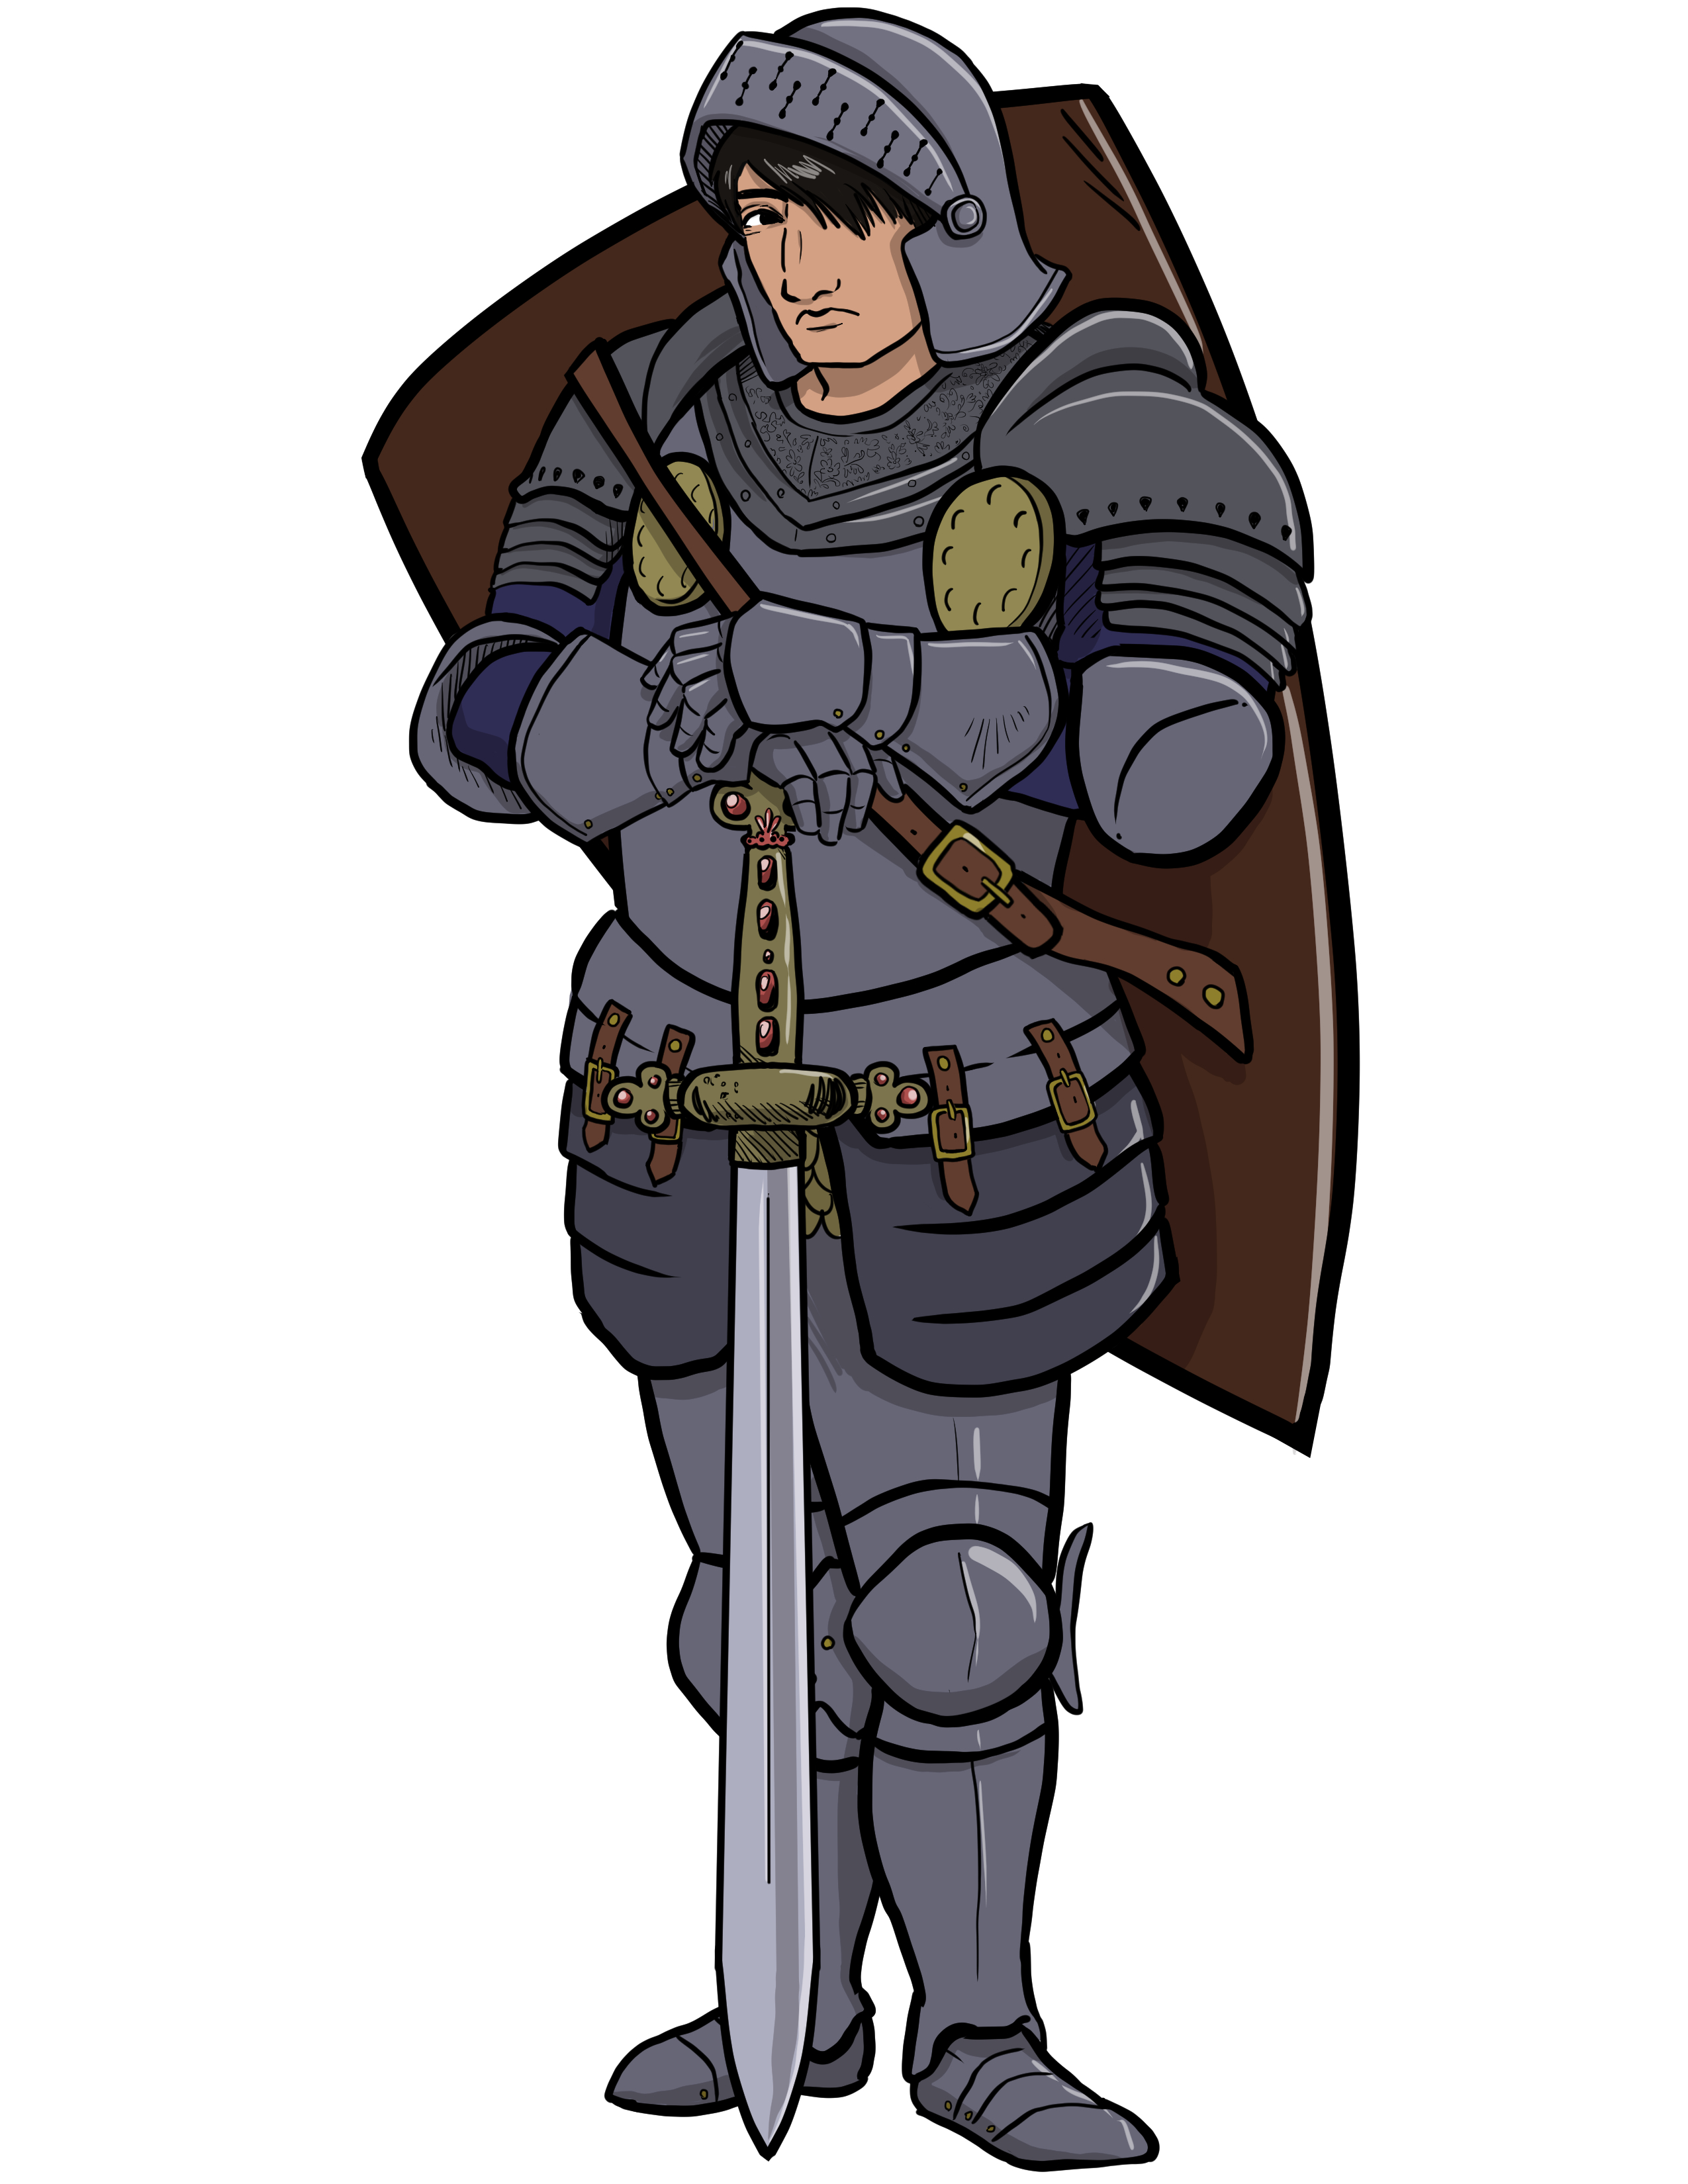
\includegraphics[width=\columnwidth]{Classes/Fighter}
Fighters are human characters who have been trained in the art of combat. They range from noble chevaliers and daring swashbucklers to brutal thugs and grizzled mercenaries.

In an adventuring party, fighters form the main front line, holding off the enemy and protecting the more vulnerable party members.

\subsection{Abilities}
\textbf{Parry:}\label{sec:Parry} At \nth{9} level, a fighter can parry incoming melee attacks. The fighter’s player declares that their character is parrying at the beginning of the round before initiative is rolled. The fighter makes no attacks during the round (and therefore needs no initiative score), but all incoming attacks are made at a -4 penalty.

If the fighter has any deflect abilities or armor class bonuses from their weapon feats, they may use them at any time during a round in which they are parrying.

\textbf{Smash:}\label{sec:Smash} At \nth{9} level, a fighter can use their brute strength to apply a harsher melee attack. The fighter automatically loses initiative, and takes a -5 penalty to their attack roll for the attack. However, if the attack hits then the fighter gets to add their \iref[sec:Strength]{Strength} score to the damage done by the attack as well as their \iref[sec:Strength]{Strength} bonus.

If the fighter has any deflect abilities or armor class bonuses from their weapon feats, they may not use them during a round in which they have smashed.

\textbf{Multiple Attacks:} At \nth{12} level, a fighter is able to make two attacks per round against any creature that they are able to hit by rolling a 2+ on the attack roll (after modifiers). At \nth{24} level, this rises to three attacks and at \nth{36} level it rises to four attacks. See \fullref{sec:Actions} for details of multiple attacks.

\statblock{\textbf{Ability Requirements:} Strength 9

\textbf{Prime Requisite:} Strength

\textbf{Hit Dice:} 1d8

\textbf{Movement:} 40 feet

\textbf{Weapons:} Any

\textbf{Armor:} Any

\textbf{Special Abilities:} Parry, Smash, Multiple Attacks}

\end{multicols*}
\begin {table}[H]
  \caption{Fighter Progression}
	\begin{tabularx}{\columnwidth}{>{\bfseries}cccM{.31in}M{.51in}M{.25in}M{.43in}M{.32in}M{.45in}Y}
    \thead{}&\thead{}&\thead{}&\thead{}&\multicolumn{5}{c}{\thead{Saving Throws}}\thead{}&\setcounter{rownum}{0}\\
    \thead{Level} & \thead{Experience} & \thead{Hit Dice} & \thead{Attack Bonus} & \thead{Death Ray/ Poison} & \thead{Magic Wands} & \thead{Paralysis/ Petrify} & \thead{Breath Weapon} & \thead{Rod/Staff/ Spell} & \thead{Special}\\
		0 & 0 & 1d4 & 0 & 14 & 15 & 16 & 17 & 17 & -\\
		1 & 0 & 1d8 & +1 & 12 & 13 & 14 & 15 & 16 & +4 Skill Points, +4 Weapon Feats\\
		2 & 2,000 & 2d8 & +1 & 12 & 13 & 14 & 15 & 16 & -\\
		3 & 4,000 & 3d8 & +2 & 11 & 12 & 13 & 14 & 15 & +1 Weapon Feat\\
		4 & 8,000 & 4d8 & +2 & 11 & 12 & 13 & 14 & 15 & -\\
		5 & 16,000 & 5d8 & +3 & 10 & 11 & 12 & 13 & 14 & +1 Skill Point\\
		6 & 32,000 & 6d8 & +4 & 9 & 10 & 11 & 12 & 13 & +1 Weapon Feat\\
		7 & 64,000 & 7d8 & +4 & 9 & 10 & 11 & 12 & 13 & -\\
		8 & 120,000 & 8d8 & +5 & 8 & 9 & 10 & 11 & 12 & -\\
		9 & 240,000 & 9d8 & +6 & 7 & 8 & 9 & 10 & 11 & Parry, Smash, +1 Skill Point, +1 Weapon Feat\\
		10 & 360,000 & 9d8+2 & +6 & 7 & 8 & 9 & 10 & 11 & -\\
		11 & 480,000 & 9d8+4 & +7 & 6 & 7 & 8 & 9 & 10 & +1 Weapon Feat\\
		12 & 600,000 & 9d8+6 & +8 & 6 & 7 & 8 & 9 & 10 & Multiple Attacks (2)\\
		13 & 720,000 & 9d8+8 & +8 & 6 & 6 & 7 & 8 & 9 & +1 Skill Point\\
		14 & 840,000 & 9d8+10 & +9 & 6 & 6 & 7 & 8 & 9 & -\\
		15 & 960,000 & 9d8+12 & +10 & 6 & 6 & 7 & 8 & 9 & +1 Weapon Feat\\
		16 & 1,080,000 & 9d8+14 & +10 & 5 & 6 & 6 & 7 & 8 & -\\
		17 & 1,200,000 & 9d8+16 & +11 & 5 & 6 & 6 & 7 & 8 & +1 Skill Point\\
		18 & 1,320,000 & 9d8+18 & +12 & 5 & 6 & 6 & 7 & 8 & -\\
		19 & 1,440,000 & 9d8+20 & +12 & 5 & 5 & 6 & 6 & 7 & +1 Weapon Feat\\
		20 & 1,560,000 & 9d8+22 & +13 & 5 & 5 & 6 & 6 & 7 & -\\
		21 & 1,680,000 & 9d8+24 & +14 & 5 & 5 & 6 & 6 & 7 & +1 Skill Point\\
		22 & 1,800,000 & 9d8+26 & +14 & 4 & 5 & 5 & 5 & 6 & -\\
		23 & 1,920,000 & 9d8+28 & +15 & 4 & 5 & 5 & 5 & 6 & +1 Weapon Feat\\
		24 & 2,040,000 & 9d8+30 & +16 & 4 & 5 & 5 & 5 & 6 & Multiple Attacks (3)\\
		25 & 2,160,000 & 9d8+32 & +16 & 4 & 4 & 5 & 4 & 5 & +1 Skill Point\\
		26 & 2,280,000 & 9d8+34 & +17 & 4 & 4 & 5 & 4 & 5 & -\\
		27 & 2,400,000 & 9d8+36 & +18 & 4 & 4 & 5 & 4 & 5 & +1 Weapon Feat\\
		28 & 2,520,000 & 9d8+38 & +18 & 3 & 4 & 4 & 3 & 4 & -\\
		29 & 2,640,000 & 9d8+40 & +19 & 3 & 4 & 4 & 3 & 4 & +1 Skill Point\\
		30 & 2,760,000 & 9d8+42 & +20 & 3 & 4 & 4 & 3 & 4 & +1 Weapon Feat\\
		31 & 2,880,000 & 9d8+44 & +20 & 3 & 3 & 3 & 2 & 3 & -\\
		32 & 3,000,000 & 9d8+46 & +21 & 3 & 3 & 3 & 2 & 3 & -\\
		33 & 3,120,000 & 9d8+48 & +22 & 3 & 3 & 3 & 2 & 3 & +1 Skill Point, +1 Weapon Feat\\
		34 & 3,240,000 & 9d8+50 & +22 & 2 & 2 & 2 & 2 & 2 & -\\
		35 & 3,360,000 & 9d8+52 & +23 & 2 & 2 & 2 & 2 & 2 & -\\
		36 & 3,480,000 & 9d8+54 & +23 & 2 & 2 & 2 & 2 & 2 & Multiple Attacks (4), +1 Weapon Feat\
  \end {tabularx}
\end {table}
\begin{multicols*}{2}

\subsection{Subclasses}
\subsubsection{Berserker}\index[classes]{Berserker}
Berserkers are tribal warriors who are known for their ferocity in battle. Outside of combat, berserkers are no more likely to be hostile than any other human.

\textbf{Rage:} When entering combat, berserkers enter an uncontrollable rage until all their enemies are vanquished. When affected by this rage berserkers gain a +2 to all attack rolls. Berserkers will fight to the death, never retreating, surrendering or taking prisoners.

This rage may also cause the berserker to attack one of their own party members. Each round, there is a 10\% chance that this will occur. The berserker will break off this attack the following round unless another 10\% is rolled.

\subsubsection{Charioteer}\index[classes]{Charioteer}
Charioteers are fighters trained in the art of driving and fighting from a chariot. They are also knowledgeable in horse care and chariot construction and repair. Most charioteers are a member of a military, although some may independent. Some of these independent charioteers may use their skills for prize tournaments.

\textbf{Chariot Combat:} When wearing any armor lighter than scale mail and with no shield equipped, charioteers suffer no penalties when fighting and driving.

At \nth{5} level charioteers can wear scale mail without suffering penalties while fighting and driving a chariot.

At \nth{8} level charioteers can use a common shield without suffering penalties while fighting and driving a chariot.

\subsubsection{Chevalier}\index[classes]{Chevalier}
After reaching \nth{9} level, a fighter who has received a title of nobility (knight or higher) might decide to take chivalric vows and dedicate themselves to a cause such as a church or a noble. Taking chivalric vows puts restrictions on the fighter’s behavior but gives them extra abilities in exchange.

A fighter wishing to take chivalric vows must first find a suitable chivalric order with which they share an alignment, and then spend a month living with the order. At the end of this time, the fighter undertakes a night long vigil, and then becomes a chevalier. Once the fighter has qualified in this way, the order places them with a particular church or noble who is a supporter of the order. The fighter may or may not get a choice of liege, but betraying a liege is considered betrayal of the order and doing so strips the chevalier of all chivalric abilities and is also likely to incur the wrath of the order.

All chevaliers must obey a strict code-of-conduct, the exact details of which will vary from order to order but will usually involve a requirement to provide hospitality and/or sanctuary to fellow chevaliers of the same order.

Lawful chevaliers are often called paladins, and chaotic chevaliers are often called avengers, but this makes no difference to the game mechanics.

\textbf{Detect Evil:} The chevalier can cast a \iref[spell:Detect Evil]{Detect Evil} spell as often as they like. Casting this spell does take the fighter’s action for a round, so cannot be done at the same time as attacking.

\textbf{Spells:} Chevaliers with a \iref[sec:Wisdom]{Wisdom} score of at least 9 can cast cleric spells as if a cleric of one third the chevalier’s level. For example a \nth{17} level chevalier can cast spells as if a \nth{6} level cleric. All the normal rules and restrictions that apply to a cleric’s casting and preparation of spells also apply to the chevalier.

\textbf{Turn Undead:} Chevaliers can turn undead as if a cleric of one third the chevalier’s level. For example a \nth{17} level chevalier can turn undead as if a \nth{6} level cleric. All the normal rules and restrictions that apply to a cleric’s turning undead also apply to the chevalier.

\paragraph{Druidic Knight}\index[classes]{Druidic Knight}\mbox{}\\
\iref[sec:Neutral]{Neutral} fighters can also become chevaliers, but only if they swear to a noble faithful to the ways of the \iref[class:Druid]{Druids}. These chevaliers are often called druidic knights.

Druidic knights do not get the Turn Undead class ability.

\textbf{Detect Danger:} The druidic knight can cast a \iref[spell:Detect Danger]{Detect Danger} spell once per hour. Casting this spell does take the fighter’s action for a round, so cannot be done at the same time as attacking.

\textbf{Spells:} Druidic knights cast druidic spells rather than clerical spells and must have a \iref[sec:Wisdom]{Wisdom} score of at least 13 to do so.

\section{Gnome}\index[classes]{Gnome}\label{class:Gnome}
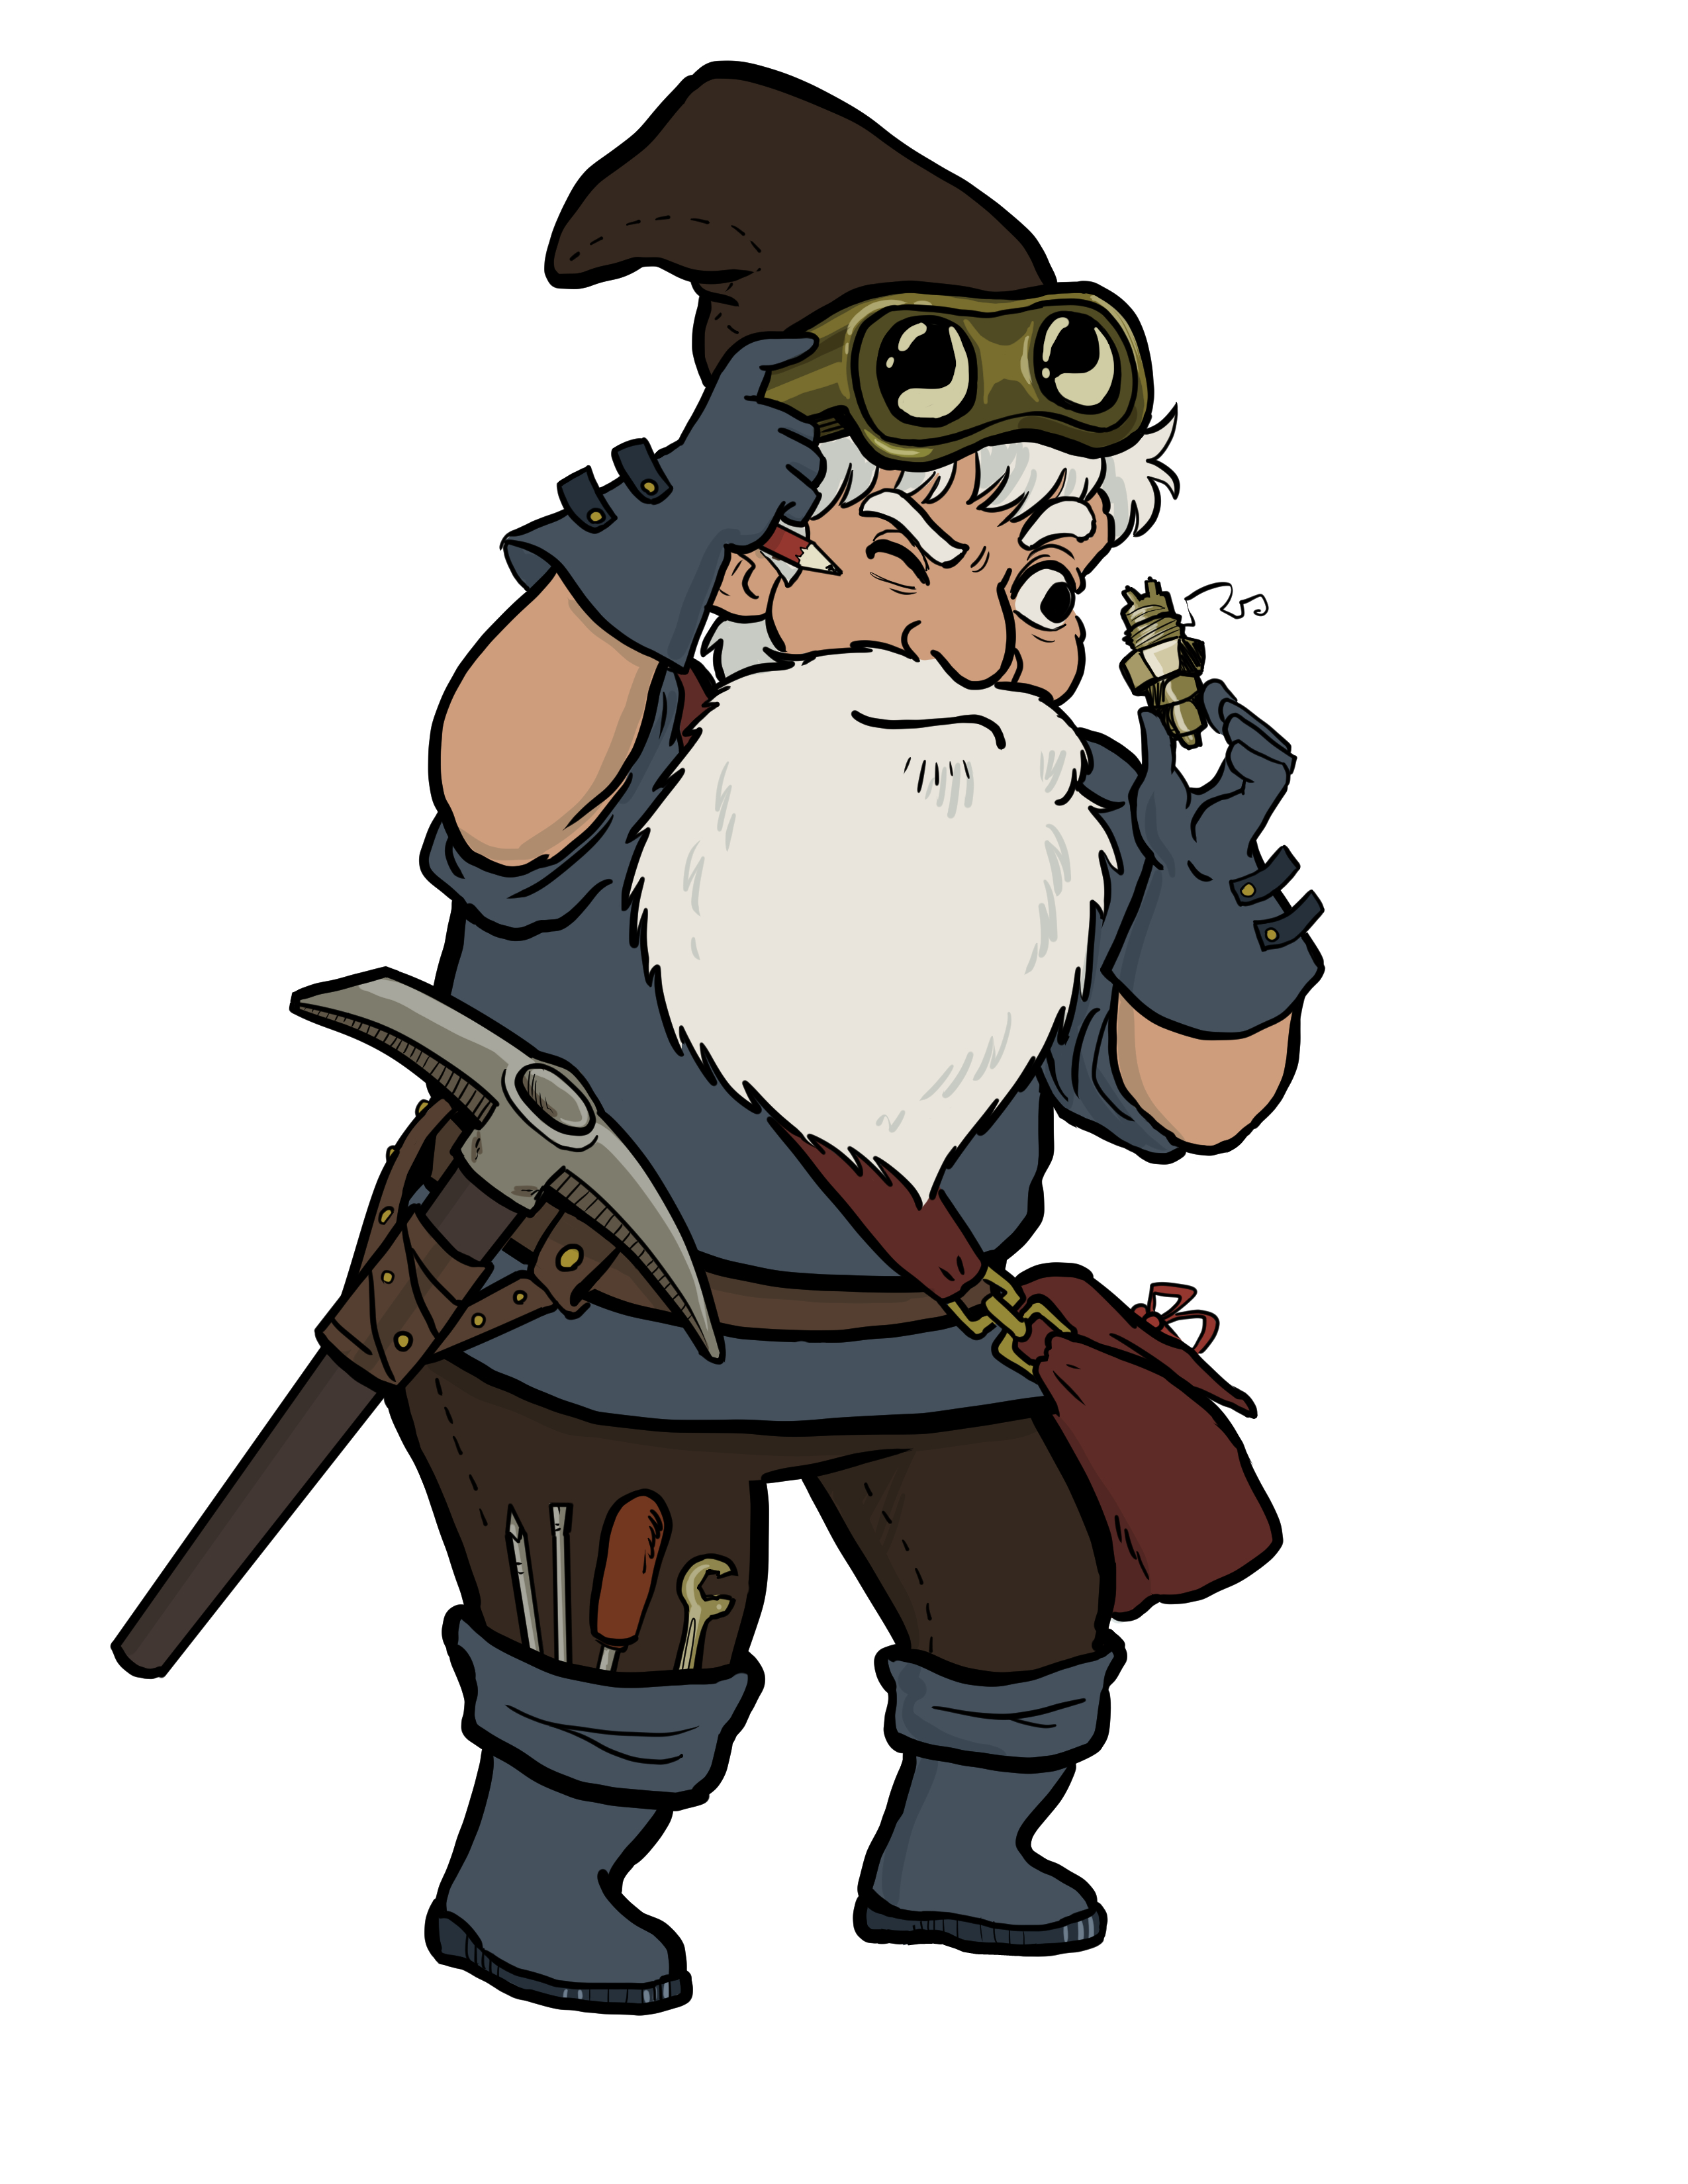
\includegraphics[width=\columnwidth]{Classes/Gnome}
Gnomes are a demi-human race. Like most demi-human races, they are less flexible than humans, and all gnome adventurers are represented by a single class.

Gnomes are small (3-4 feet) humanoids distantly related to dwarves. They look like small humans with long noses and beards but bald heads. Like dwarves, the women have beards like the men.

Gnomes are excellent miners, specializing in mining gems and red powder.

Gnomes are excellent tinkerers and inventors, and love anything mechanical. They are very proud of the fact that guns are a gnomish invention.

Unlike their dwarven cousins, gnomes are very magical. They may use any magic item (even those normally only usable by a particular class).

Gnome adventurers make reasonably skilled warriors who are at home in underground environments.

\subsection{Abilities}
\textbf{Infravision:} Gnomes have \iref[sec:Infravision]{Infravision} (see \fullref{sec:Infravision}).

\textbf{Stonelore:} At \nth{7} level and higher, a gnome’s experience with mining gives them a chance to detect irregularities in construction. If a gnome examines an area looking for irregularities, the Game Master should secretly roll 1d6 for each feature in the area being searched that is one of the following:

\begin{itemize}
	\item{Traps involving moving stone walls or blocks of stone}
	\item{Secret doors involving moving stone walls.}
	\item{Newly built stone constructions.}
	\item{Gently sloping stonework.}
\end{itemize}
In each case, if the 1d6 roll is a 1-2, the gnome is able to detect the feature. If the roll is a 3-6, then the gnome in unable to detect the feature (and the gnome’s player should not be told whether this was because the roll failed or because there was no feature to detect).

\textbf{Resistance to Earth Attacks:} At \nth{8} level and higher, a gnome gains a +1 bonus on saving throws versus earth-based attacks; including acid (e.g. black dragon breath) and petrification (e.g., the touch of a cockatrice).

At \nth{11} level and higher, this bonus becomes a +2.

\textbf{Small:} By \nth{9} level, gnomes have learned to use their small size to avoid larger creatures in combat. Gnomes gain a -1 bonus to armor class against attacks from creatures of larger than human size.

\textbf{Speak with Burrowing Animals:} At \nth{10} level, a gnome gains the ability to communicate with burrowing animals such as badgers, moles, etc. When communicating, the gnome’s player should keep in mind that these animals are not that intelligent.

\textbf{Fighter Abilities:} At \nth{11} level and higher, a gnome can use the following fighter abilities: Parry and Smash, and Multiple Attacks (at \nth{11} and \nth{18} level).

\textbf{Greasemonkey:} At \nth{12} level and higher, a gnome gains a +1 bonus on checks involving machinery.

\textbf{Wall of Stone:} At \nth{13} level, a gnome gains the ability to cast a Wall of Stone once per week as a \nth{9} level wizard. This can only be done if the gnome is underground, with no direct access to the sky. If this ability is used in the gnome’s home burrow, the wall can be twice the normal size.

\textbf{Miracle Worker:} At \nth{14} level and higher, a gnome gains a +2 bonus on all Engineering skill checks when designing machinery. If the check is successful the device works as expected even tho it doesn’t look like it should.

\statblock{\textbf{Ability Requirements:} Constitution 9, Intelligence 9

\textbf{Prime Requisite:} Strength and Dexterity

\textbf{Ability Modifiers:} Intelligence +1, Wisdom -1

\textbf{Hit Dice:} 1d6

\textbf{Movement:} 20 feet

\textbf{Weapons:} Any small

\textbf{Armor:} Any except large shields

\textbf{Special Abilities:} Infravision, Stonelore, Resistance to Earth Attacks, Small, Speak with Burrowing Animals, Multiple Attacks, Parry, Smash, Greasemonkey, Wall of Stone, Miracle Worker

\textbf{Required Skills:} Craft (Machine Building), Engineering}

\end{multicols*}
\begin {table}[H]
  \caption{Gnome Progression}
	\begin{tabularx}{\columnwidth}{>{\bfseries}cccM{.31in}M{.51in}M{.25in}M{.43in}M{.32in}M{.45in}Y}
    \thead{}&\thead{}&\thead{}&\thead{}&\multicolumn{5}{c}{\thead{Saving Throws}}\thead{}&\setcounter{rownum}{0}\\
    \thead{Level} & \thead{Experience} & \thead{Hit Dice} & \thead{Attack Bonus} & \thead{Death Ray/ Poison} & \thead{Magic Wands} & \thead{Paralysis/ Petrify} & \thead{Breath Weapon} & \thead{Rod/Staff/ Spell} & \thead{Special}\\
		1 & 0 & 1d6 & +1 & 8 & 9 & 10 & 13 & 12 & Infravision\\
		2 & 2,000 & 2d6 & +1 & 8 & 9 & 10 & 13 & 12 & -\\
		3 & 4,000 & 3d6 & +2 & 7 & 8 & 9 & 12 & 11 & -\\
		4 & 8,000 & 4d6 & +2 & 6 & 7 & 8 & 10 & 9 & -\\
		5 & 16,000 & 5d6 & +3 & 5 & 6 & 7 & 9 & 8 & -\\
		6 & 32,000 & 6d6 & +4 & 4 & 5 & 6 & 8 & 7 & -\\
		7 & 64,000 & 7d6 & +4 & 3 & 4 & 5 & 6 & 5 & Stonelore\\
		8 & 120,000 & 8d6 & +5 & 2 & 3 & 4 & 5 & 4 & Resistance to Earth Attacks (+1)\\
		9 & 300,000 & 9d6 & +6 & 2 & 3 & 4 & 5 & 4 & Small\\
		10 & 600,000 & 9d6+1 & +6 & 2 & 2 & 3 & 4 & 3 & Speak with Burrowing Animals\\
		11 & 900,000 & 9d6+2 & +7 & 2 & 2 & 3 & 4 & 3 & Multiple Attacks, Parry, Resistance to Earth Attacks (+2), Smash\\
		12 & 1,200,000 & 9d6+3 & +8 & 2 & 2 & 2 & 3 & 2 & Greasemonkey\\
		13 & 1,500,000 & 9d6+4 & +8 & 2 & 2 & 2 & 3 & 2 & Wall of Stone\\
		14 & 1,800,000 & 9d6+5 & +9 & 2 & 2 & 2 & 2 & 2 & Miracle Worker\\
		15 & 2,100,000 & 9d6+6 & +10 & 2 & 2 & 2 & 2 & 2 & -\\
		16 & 2,400,000 & 9d6+7 & +10 & 2 & 2 & 2 & 2 & 2 & -\\
		17 & 2,700,000 & 9d6+8 & +11 & 2 & 2 & 2 & 2 & 2 & -\\
		18 & 3,000,000 & 9d6+9 & +12 & 2 & 2 & 2 & 2 & 2 & Multiple Attacks (3)\\
		19 & 3,200,000 & 9d6+10 & +12 & 2 & 2 & 2 & 2 & 2 & -\\
		20 & 3,400,000 & 9d6+11 & +13 & 2 & 2 & 2 & 2 & 2 & -\\
		21 & 3,600,000 & 9d6+12 & +14 & 2 & 2 & 2 & 2 & 2 & -\\
		22 & 3,800,000 & 9d6+13 & +14 & 2 & 2 & 2 & 2 & 2 & -\\
		23 & 4,000,000 & 9d6+14 & +15 & 2 & 2 & 2 & 2 & 2 & -\\
		24 & 4,200,000 & 9d6+15 & +16 & 2 & 2 & 2 & 2 & 2 & -\\
		25 & 4,400,000 & 9d6+16 & +16 & 2 & 2 & 2 & 2 & 2 & -\\
		26 & 4,600,000 & 9d6+17 & +17 & 2 & 2 & 2 & 2 & 2 & -\\
		27 & 4,800,000 & 9d6+18 & +18 & 2 & 2 & 2 & 2 & 2 & -\\
		28 & 5,000,000 & 9d6+19 & +18 & 2 & 2 & 2 & 2 & 2 & -\\
		29 & 5,200,000 & 9d6+20 & +19 & 2 & 2 & 2 & 2 & 2 & -\\
		30 & 5,400,000 & 9d6+21 & +20 & 2 & 2 & 2 & 2 & 2 & -\\
		31 & 5,600,000 & 9d6+22 & +20 & 2 & 2 & 2 & 2 & 2 & -\\
		32 & 5,800,000 & 9d6+23 & +21 & 2 & 2 & 2 & 2 & 2 & -\\
		33 & 6,000,000 & 9d6+24 & +22 & 2 & 2 & 2 & 2 & 2 & -\\
		34 & 6,200,000 & 9d6+25 & +22 & 2 & 2 & 2 & 2 & 2 & -\\
		35 & 6,400,000 & 9d6+26 & +23 & 2 & 2 & 2 & 2 & 2 & -\\
		36 & 6,600,000 & 9d6+27 & +23 & 2 & 2 & 2 & 2 & 2 & -\
  \end {tabularx}
\end {table}
\newpage
\begin{multicols*}{2}

\section{Halfling}\index[classes]{Halfling}\label{class:Halfling}
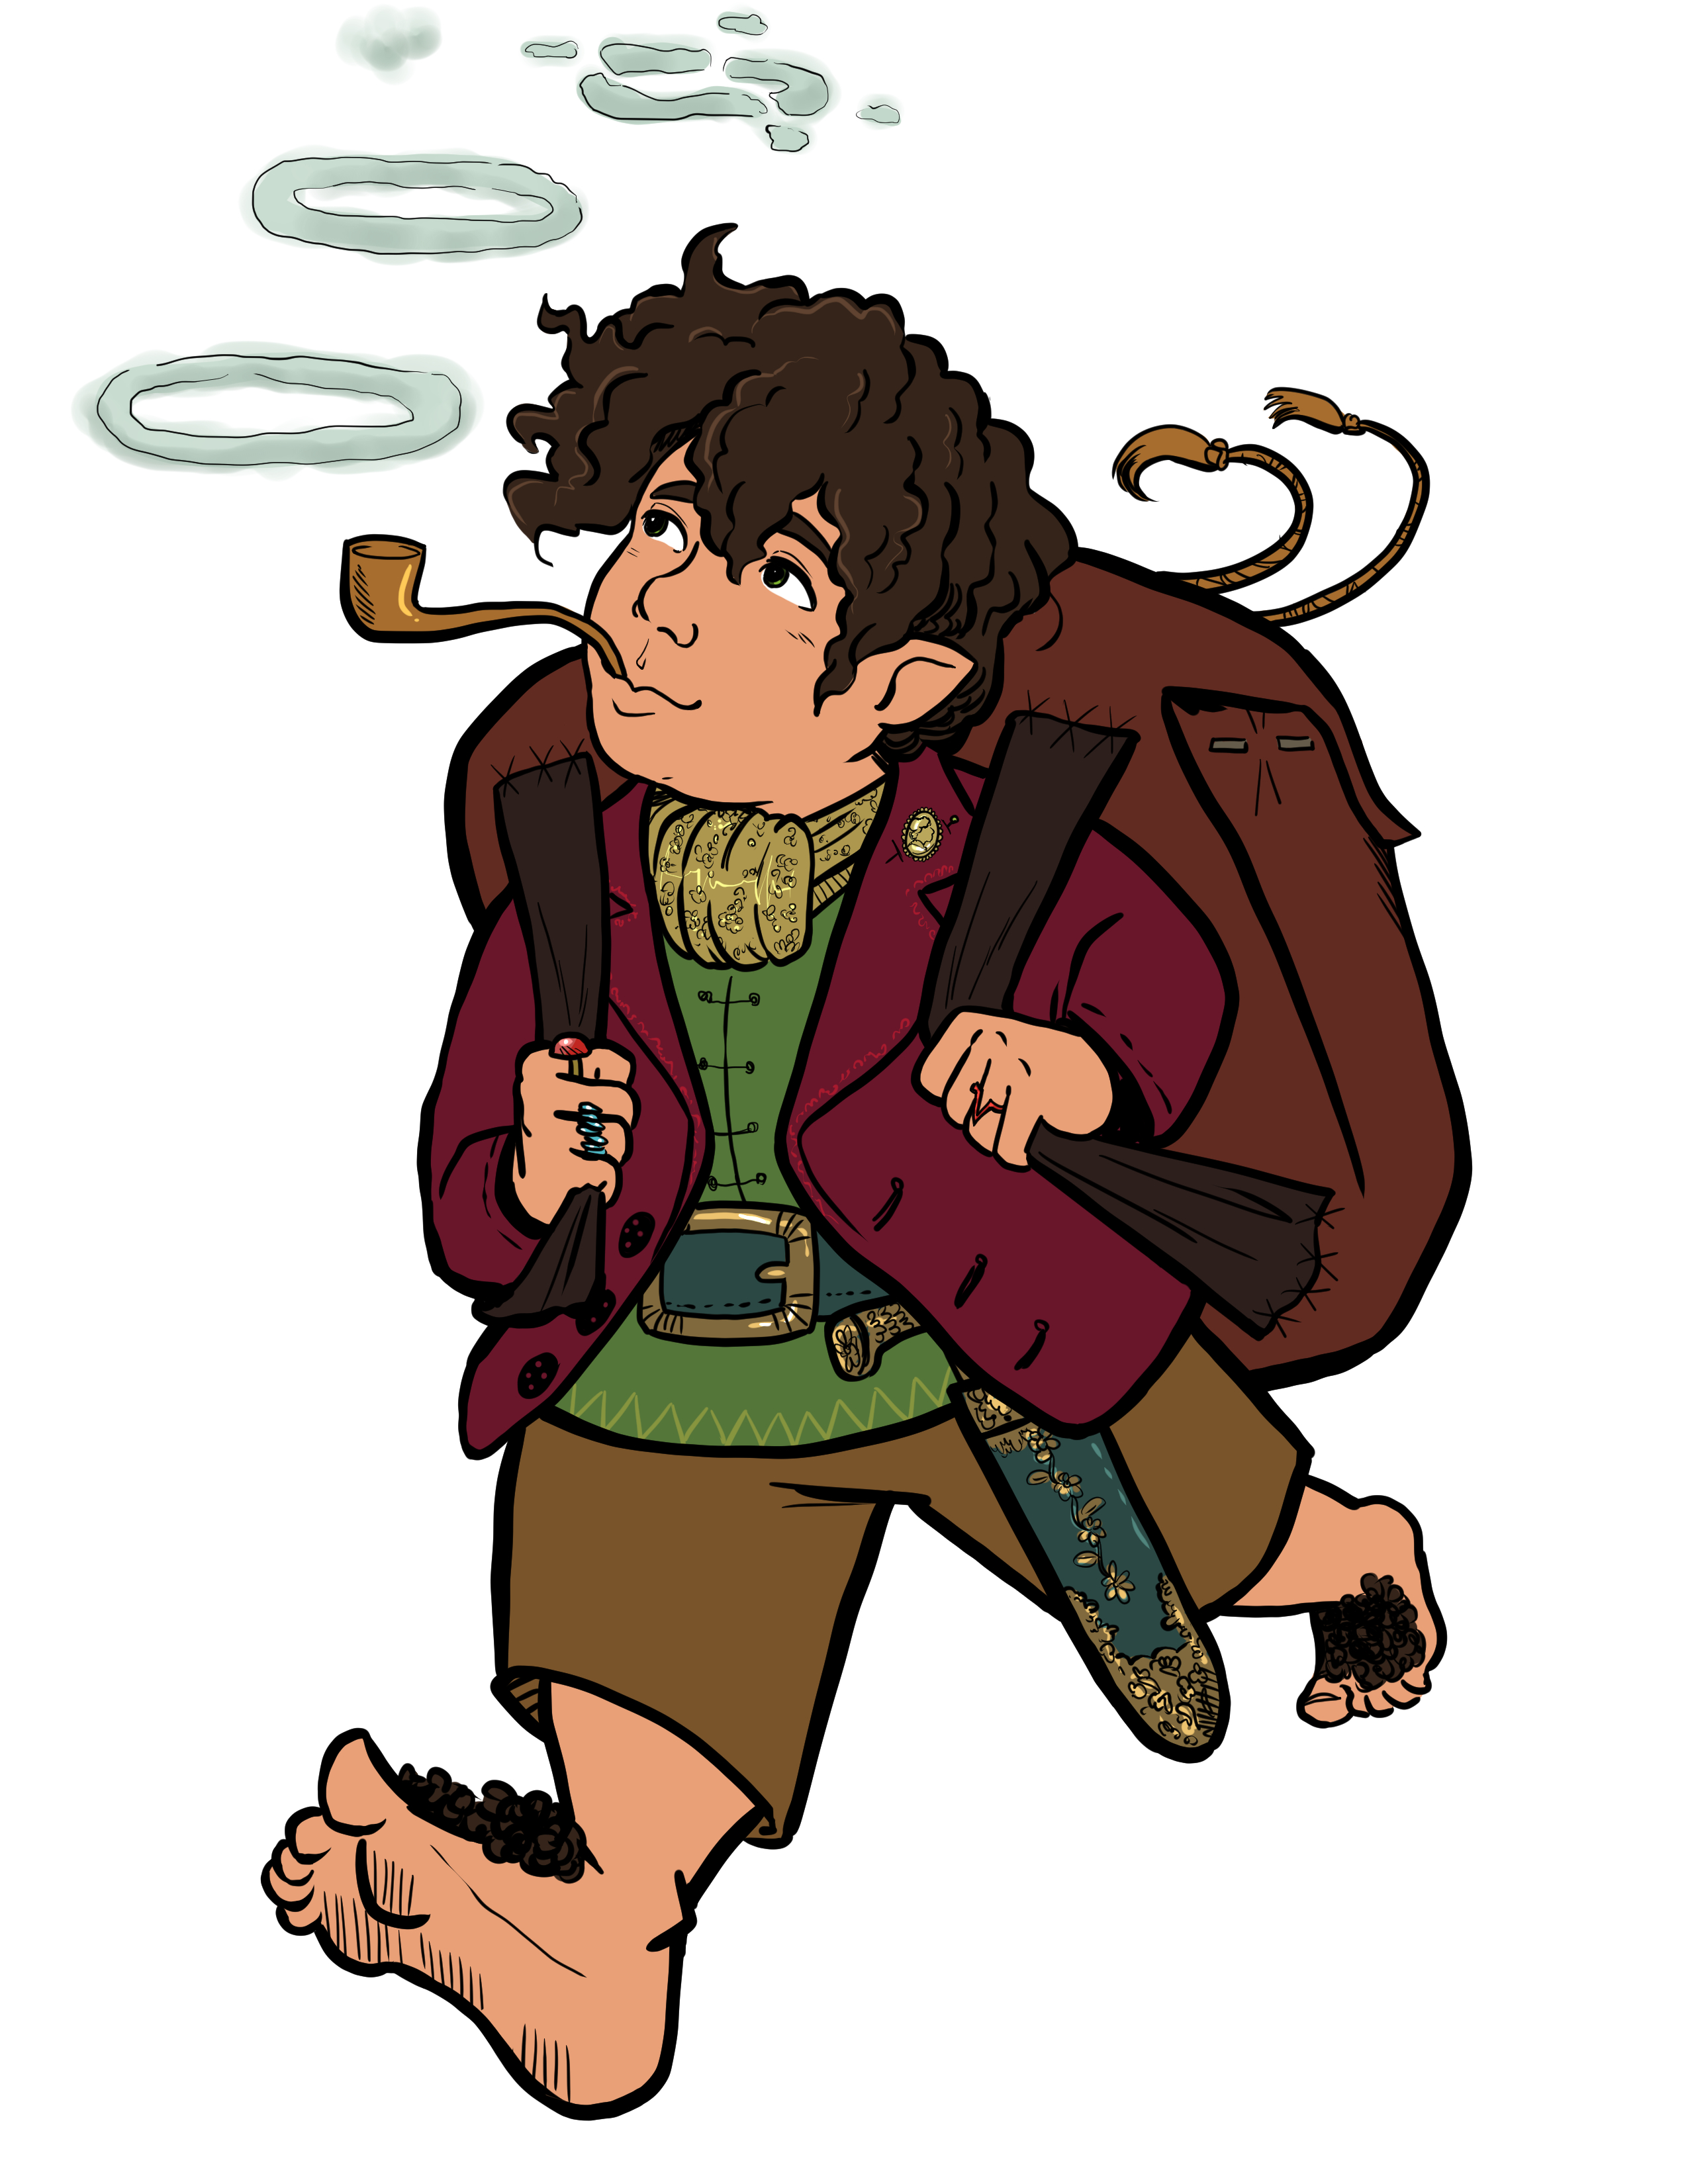
\includegraphics[width=\columnwidth]{Classes/Halfling}
Halflings are a demi-human race. Like most demi-human races, they are less flexible than humans, and all halfling adventurers are represented by a single class.

Halflings are much shorter and lighter than humans, standing only 3 feet tall. They are of a proportionally similar build to humans, with the exception of their feet—which are large and covered in hair. The soles of halflings feet are tough and resilient, and halflings often travel bare-footed.

Halflings’ skin tone has a similar range to that of humans, as does their hair color. Halflings do not grow beards or mustaches, but the sideburns of adult males tend to be longer than those of humans.

Like dwarves, halflings are an inherently non-magical race, and possess no magic users or clerics of their own. They share the dwarves’ natural resilience and resistance to magical attacks, and although they are not as physically tough and adept at fighting as dwarves they make up for this with their natural stealth.

Halflings are very gregarious and can be commonly found living amongst humans and other demi-humans. If left to themselves, they form small villages in grasslands and hills where they excel at farming.

Halfling food production and the halfling love of cookery and brewing make them very popular amongst the other races.

Halfling adventurers make reasonably skilled warriors and scouts who excel in outdoor environments.

\subsection{Abilities}
\textbf{Infravision:} Halflings have \iref[sec:Infravision]{Infravision} (see \fullref{sec:Infravision}).

\textbf{Nimble:} A halfling’s natural agility gives it a +1 bonus to attack rolls when using any missile weapon and a +1 bonus to initiative rolls.

\textbf{Small:} Halflings’ small size makes it hard for larger creatures to hit them. Halflings gain a -2 bonus to armor class against attacks from creatures of larger than human size.

\textbf{Unobtrusive:} In outdoor surroundings, a halfling who remains still can hide with a 90\% chance of success providing there are bushes, rocks or trees that can be used as cover. Indoors, a halfling who remains still can hide with a 33\% chance of success as long as there is cover or shadow available.

Halflings use this ability to hide in natural daylight, but magical light such as that from a \iref[spell:Continual Light]{Continual Light} spell prevents this ability from working.

\textbf{Disavowal:} At \nth{5} level and higher, a halfling gains the ability to stop a magical effect. This can be done once every 24 hours, but only while the halfling is within a halfling shire. To activate this ability, the halfling must focus their will at the target and yell "No!". The halfling than takes 1d4 points of damage. Even if this damage would kill the halfling, the ability is still successful.

\textbf{Spell Resistance:} At \nth{9} level and higher, a halfling only takes half damage from all spells and spell-like abilities. If the attack normally allows a saving throw for half damage then the halfling only takes a quarter of normal damage if they save successfully.

\textbf{Fighter Abilities:} At \nth{11} level and higher, a halfling can use the following fighter abilities: Parry and Smash, and Multiple Attacks (at \nth{11} and \nth{18} level).

\textbf{Breath Evasion:} At \nth{15} level and higher, a halfling only takes half damage from all breath weapons such as those used by dragons. If the attack normally allows a saving throw for half damage then the halfling only takes a quarter of normal damage if they save successfully.

\statblock{\textbf{Ability Requirements:} Dexterity 9, Constitution 9

\textbf{Prime Requisite:} Strength and Dexterity

\textbf{Ability Modifiers:} Strength -1, Dexterity +1

\textbf{Hit Dice:} 1d6

\textbf{Movement:} 30 feet

\textbf{Weapons:} Any small, light crossbow, short bow

\textbf{Armor:} Any except large shields

\textbf{Special Abilities:} Infravision, Nimble, Small, Unobtrusive, Disavowal, Spell Resistance, Multiple Attacks, Smash, Parry, Breath Evasion}

\end{multicols*}
\begin {table}[H]
  \caption{Halfling Progression}
	\begin{tabularx}{\columnwidth}{>{\bfseries}cccM{.31in}M{.51in}M{.25in}M{.43in}M{.32in}M{.45in}Y}
    \thead{}&\thead{}&\thead{}&\thead{}&\multicolumn{5}{c}{\thead{Saving Throws}}\thead{}&\setcounter{rownum}{0}\\
    \thead{Level} & \thead{Experience} & \thead{Hit Dice} & \thead{Attack Bonus} & \thead{Death Ray/ Poison} & \thead{Magic Wands} & \thead{Paralysis/ Petrify} & \thead{Breath Weapon} & \thead{Rod/Staff/ Spell} & \thead{Special}\\
		1 & 0 & 1d6 & +1 & 8 & 9 & 10 & 13 & 12 & Nimble, Small, Unobtrusive, +4 Skill Points, +2 Weapon Feats\\
		2 & 2,000 & 2d6 & +1 & 8 & 9 & 10 & 13 & 12 & -\\
		3 & 4,000 & 3d6 & +1 & 7 & 8 & 9 & 12 & 11 & +1 Weapon Feat\\
		4 & 8,000 & 4d6 & +2 & 6 & 7 & 8 & 10 & 9 & -\\
		5 & 16,000 & 5d6 & +2 & 5 & 6 & 7 & 9 & 8 & Disavowal, +1 Skill Point\\
		6 & 32,000 & 6d6 & +3 & 4 & 5 & 6 & 8 & 7 & +1 Weapon Feat\\
		7 & 64,000 & 7d6 & +3 & 3 & 4 & 5 & 6 & 5 & -\\
		8 & 120,000 & 8d6 & +4 & 2 & 3 & 4 & 5 & 4 & -\\
		9 & 300,000 & 9d6 & +4 & 2 & 3 & 4 & 5 & 4 & Spell Resistance, +1 Skill Point, +1 Weapon Feat\\
		10 & 600,000 & 9d6+1 & +5 & 2 & 2 & 3 & 4 & 3 & -\\
		11 & 900,000 & 9d6+2 & +5 & 2 & 2 & 3 & 4 & 3 & Multiple Attacks, Parry, Smash, +1 Weapon Feat\\
		12 & 1,200,000 & 9d6+3 & +6 & 2 & 2 & 2 & 3 & 2 & -\\
		13 & 1,500,000 & 9d6+4 & +6 & 2 & 2 & 2 & 3 & 2 & +1 Skill Point\\
		14 & 1,800,000 & 9d6+5 & +7 & 2 & 2 & 2 & 2 & 2 & -\\
		15 & 2,100,000 & 9d6+6 & +7 & 2 & 2 & 2 & 2 & 2 & Breath Evasion, +1 Weapon Feat\\
		16 & 2,400,000 & 9d6+7 & +8 & 2 & 2 & 2 & 2 & 2 & -\\
		17 & 2,700,000 & 9d6+8 & +8 & 2 & 2 & 2 & 2 & 2 & +1 Skill Point\\
		18 & 3,000,000 & 9d6+9 & +9 & 2 & 2 & 2 & 2 & 2 & Multiple Attacks (3)\\
		19 & 3,200,000 & 9d6+10 & +9 & 2 & 2 & 2 & 2 & 2 & -\\
		20 & 3,400,000 & 9d6+11 & +10 & 2 & 2 & 2 & 2 & 2 & -\\
		21 & 3,600,000 & 9d6+12 & +10 & 2 & 2 & 2 & 2 & 2 & +1 Skill Point\\
		22 & 3,800,000 & 9d6+13 & +11 & 2 & 2 & 2 & 2 & 2 & -\\
		23 & 4,000,000 & 9d6+14 & +11 & 2 & 2 & 2 & 2 & 2 & +1 Weapon Feat\\
		24 & 4,200,000 & 9d6+15 & +12 & 2 & 2 & 2 & 2 & 2 & -\\
		25 & 4,400,000 & 9d6+16 & +12 & 2 & 2 & 2 & 2 & 2 & +1 Skill Point\\
		26 & 4,600,000 & 9d6+17 & +13 & 2 & 2 & 2 & 2 & 2 & -\\
		27 & 4,800,000 & 9d6+18 & +13 & 2 & 2 & 2 & 2 & 2 & -\\
		28 & 5,000,000 & 9d6+19 & +14 & 2 & 2 & 2 & 2 & 2 & -\\
		29 & 5,200,000 & 9d6+20 & +14 & 2 & 2 & 2 & 2 & 2 & +1 Skill Point\\
		30 & 5,400,000 & 9d6+21 & +15 & 2 & 2 & 2 & 2 & 2 & +1 Weapon Feat\\
		31 & 5,600,000 & 9d6+22 & +15 & 2 & 2 & 2 & 2 & 2 & -\\
		32 & 5,800,000 & 9d6+23 & +16 & 2 & 2 & 2 & 2 & 2 & -\\
		33 & 6,000,000 & 9d6+24 & +16 & 2 & 2 & 2 & 2 & 2 & +1 Skill Point\\
		34 & 6,200,000 & 9d6+25 & +17 & 2 & 2 & 2 & 2 & 2 & -\\
		35 & 6,400,000 & 9d6+26 & +17 & 2 & 2 & 2 & 2 & 2 & -\\
		36 & 6,600,000 & 9d6+27 & +18 & 2 & 2 & 2 & 2 & 2 & +1 Weapon Feat\
  \end {tabularx}
\end {table}
\newpage
\begin{multicols*}{2}

\section{Monk}\index[classes]{Monk}\label{class:Monk}
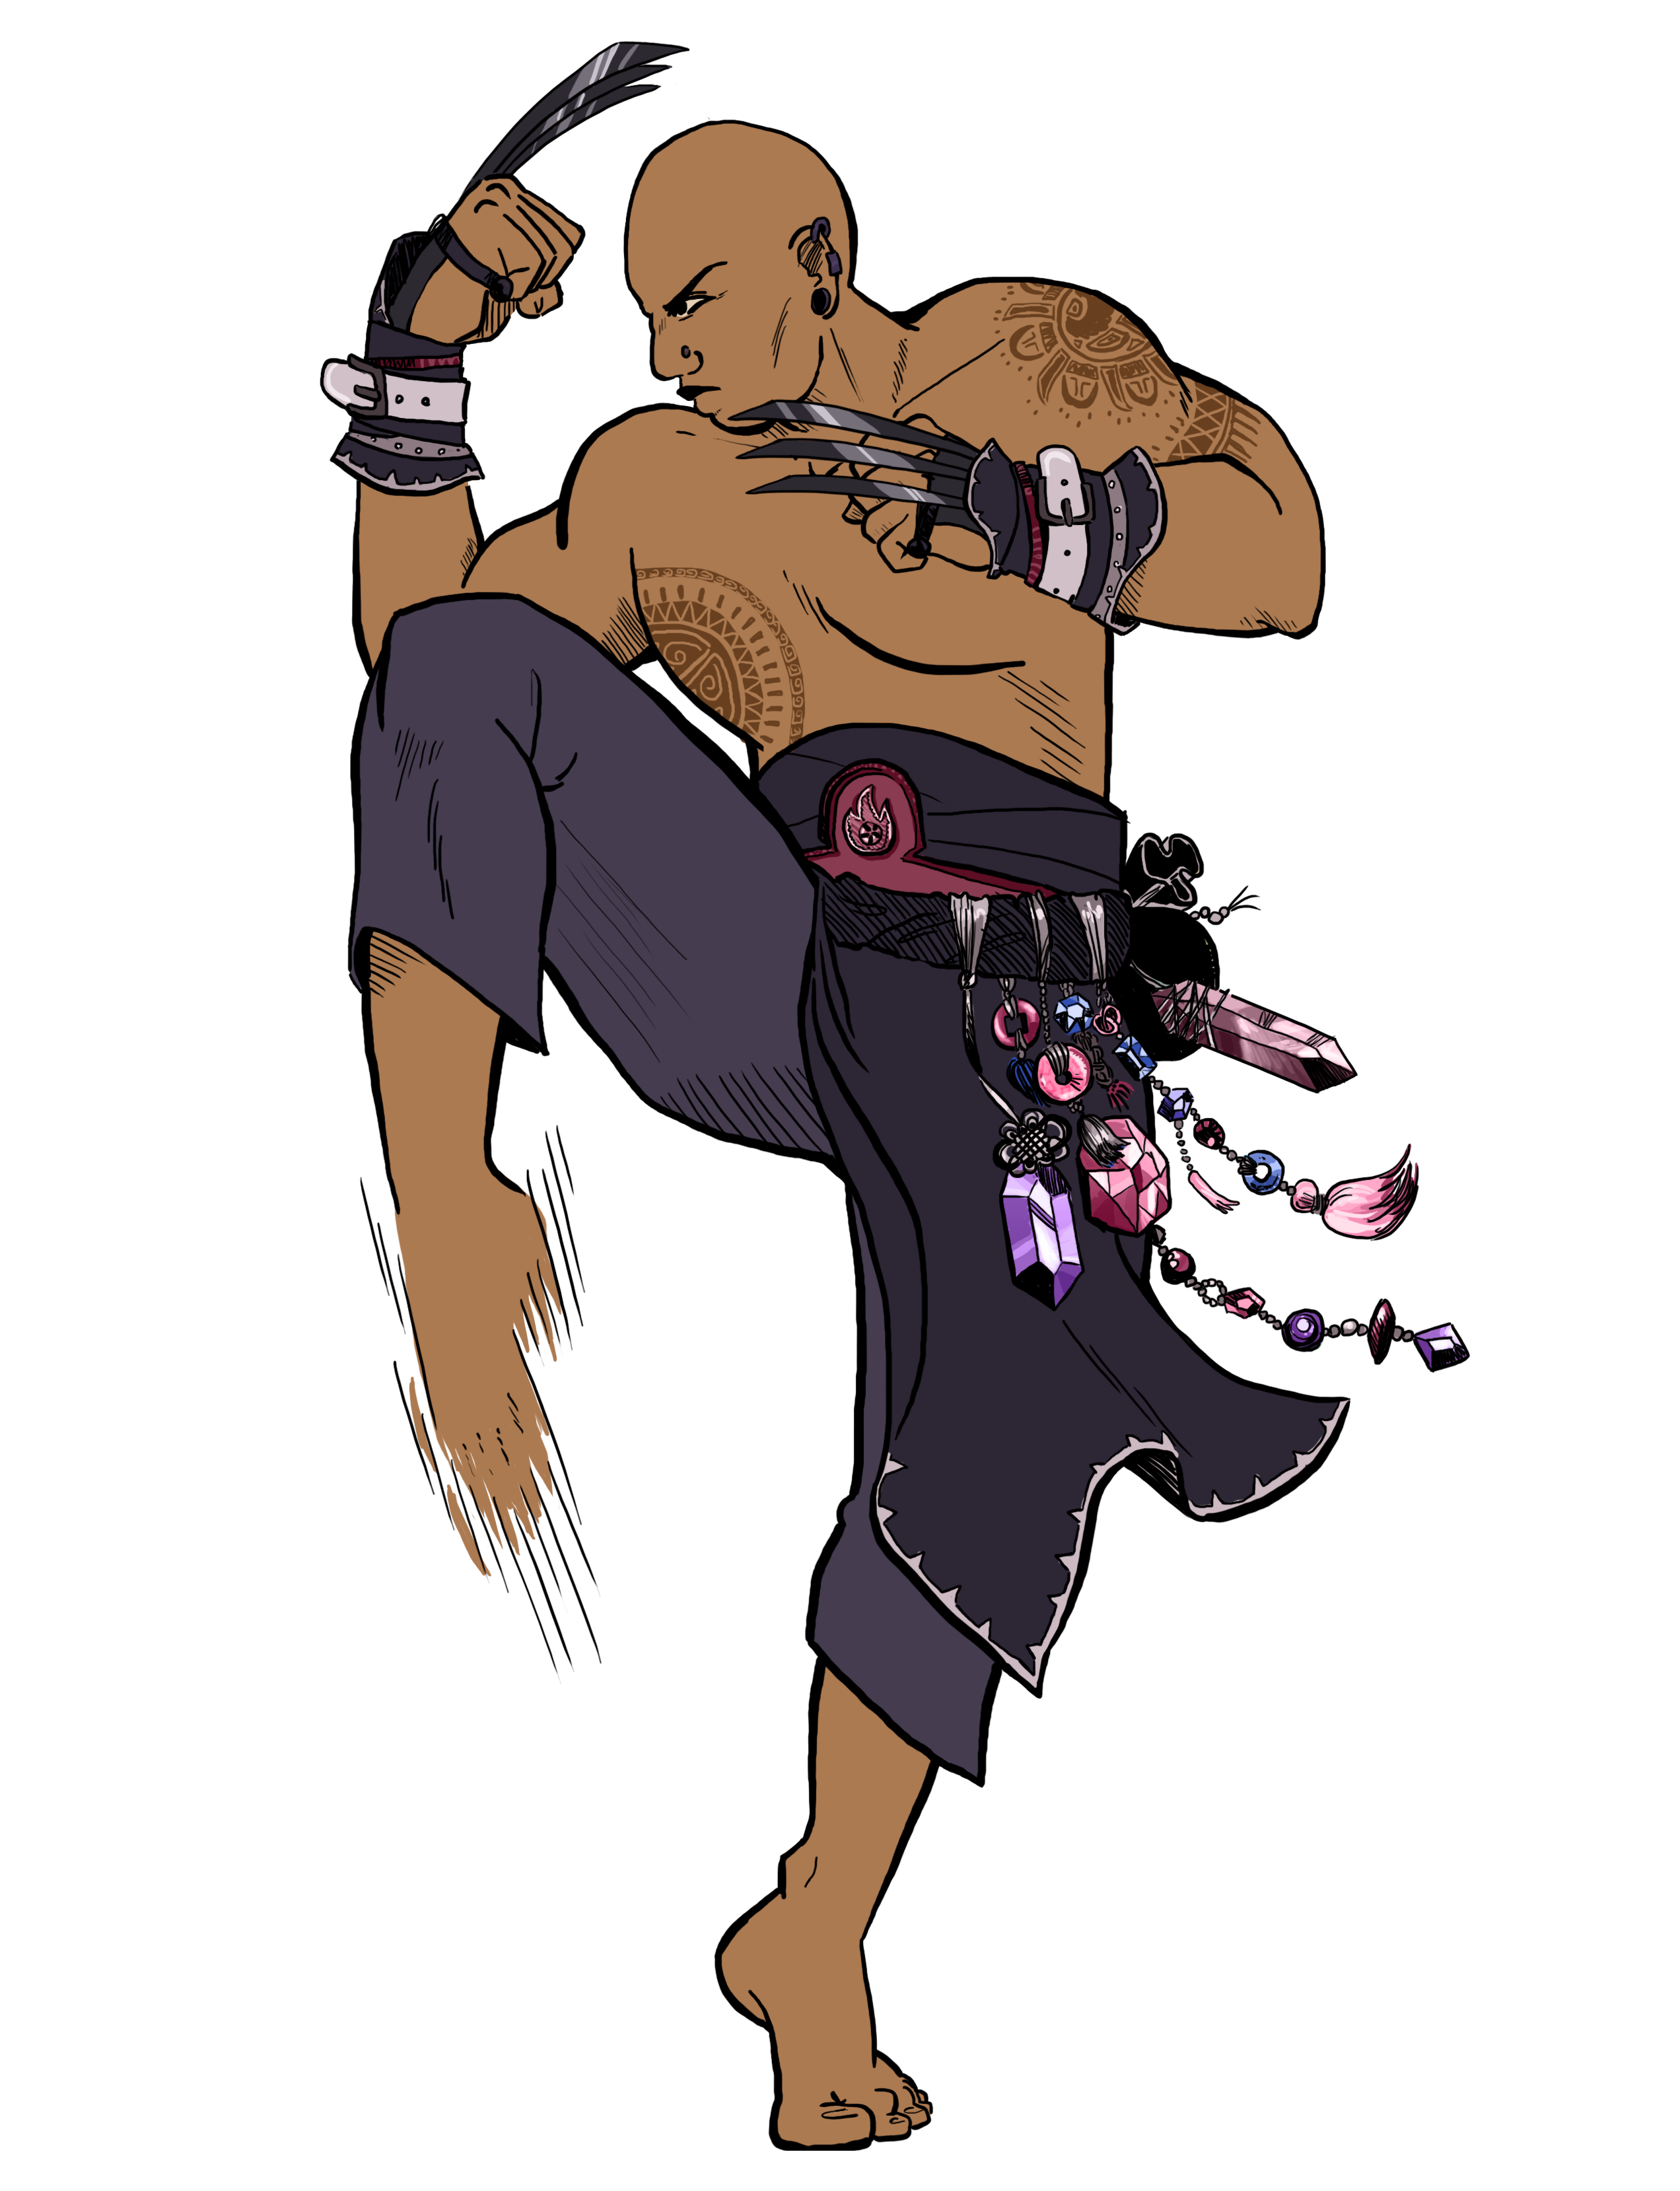
\includegraphics[width=\columnwidth]{Classes/Monk}
Monks are human characters who have undergone intense physical and mental training in order to unlock their inner potential via martial arts and meditation.

Monks are trained in isolated monasteries where they live an ascetic life in seclusion from the distractions of the civilized world. While many are content to live their lives in these monasteries, some venture out into the world once their training is complete—whether from a desire to do good deeds or from a desire to use their talents for personal gain.

The special monk training allows the character to exceed normal human limits. Their incredible speed and agility provides them with unsurpassed ability in unarmed combat.

However, monks that wander away from their monastery must still obey the code of behavior instilled into them during their training if they are to keep their minds strong enough to use their abilities. This code consists of:

\begin{itemize}
	\item{\textit{Never tell an untruth.} Dissembling and lies of omission are acceptable, but not knowingly false statements.}
	\item{\textit{Own only what you can carry.} A wandering monk must be able to travel freely without concern for goods and homes left behind, and is therefore forbidden by their code from owning any possessions they can not personally carry around with them. Note that this is not a vow of poverty. A monk is allowed by their code to be wealthy, as long as their riches are portable.}
	\item{\textit{Trust your abilities.} A monk who doubts their own abilities lacks the confidence to use them properly, therefore the code does not allow monks to augment the defensive capabilities of their discipline (i.e. their natural armor class) with magic or mundane means.}
\end{itemize}
Within an adventuring party, monks can prove to be able warriors, though not quite as able as fighters; and back this talent up with useful scouting skills.

\subsection{Abilities}
\textbf{Rogue Abilities:} Monks can use the following rogue abilities as if they were a rogue of the same level: Climb Walls, Find Traps, Hide in Shadows, Move Silently, and Remove Traps.

\textbf{Strike to Kill Damage:} When attacking while unarmed, a monk can choose to do strike to kill when using the Unarmed Strike weapon feat instead of striking to stun (see \fullref{chap:Weapon Feats}). If they do so, they do more damage (and \iref[sec:Strength]{Strength} bonuses apply as normal), but lose the chance to stun or knock out their opponent.

This damage starts at 1d4 at \nth{1} level, and increases with level until it reaches a maximum of 3d12 damage at \nth{16} level. The damage done by a monk of a particular level is listed on \fullref{tab:Monk Special Abilities Progression}.

\textbf{Unarmed Attack As:} Because of the semi-magical nature of a monk’s martial arts, their unarmed attacks (whether striking to stun or to kill) count as if they are magical for the purposes of determining whether they can affect creatures who may be immune to non-magical weapons.

At \nth{2} level a monk’s unarmed attacks can hit creatures only hurt by silver weapons, and at \nth{5} level they can start to hit creatures only hit by magic weapons. The effective bonus of the monk’s attacks continues to increase as listed in \fullref{tab:Monk Special Abilities Progression}.

It is important to note that this bonus is only used to determine whether or not a monk is capable of hurting an opponent. The monk does not actually get this bonus on their to hit or damage rolls.

\textbf{Alertness:} When a fight suddenly breaks out, or when two groups come face to face abruptly, a \nth{2} level or higher monk is only surprised (see \fullref{sec:Surprise}) if their player rolls a 1 on a d6, rather than the normal 1-2 on a d6.

\textbf{Self Healing:} Starting at \nth{4} level, once per day, a monk can spend a round concentrating and heal themselves 1 hit point per level that they have.

\textbf{Strike to Kill Attacks:} When a monk reaches \nth{5} level, they can make two attacks per round while they are unarmed and attacking using their martial arts to kill their opponents.

They do not get the extra attack when using weapons or when using the Unarmed Strike weapon feat to stun foes (see \fullref{chap:Weapon Feats}). At \nth{9} level this increases to three attacks per round, and at \nth{13} level it increases again to 4 attacks per round.

\textbf{Speak with Animals:} A \nth{6} level or higher monk is able to understand the speech of any animal, and is able to make any animal understand their speech. This is a mental ability, not a physical one. If conversing with a dog, the monk does not actually growl and bark but talks normally—reaching into the dog’s mind to make it understand.

This ability does not bestow any extra intelligence to the animal. Neither does it force the animal to obey or even co-operate with the monk.

\textbf{Spell Resistance:} At \nth{8} level and higher, a monk only takes half damage from all spells and spell-like abilities. If the attack normally allows a saving throw for half damage then the monk only takes a quarter of normal damage if they save successfully.

\textbf{Breath Evasion:} At \nth{8} level and higher, a monk only takes half damage from all breath weapons such as those used by dragons. If the attack normally allows a saving throw for half damage then the monk only takes a quarter of normal damage if they save successfully.

\textbf{Fighter Abilities:} At \nth{9} level and higher, a monk can use the following fighter abilities: \iref[sec:Parry]{Parry} and \iref[sec:Smash]{Smash}.

\textbf{Speak with Anyone:} At \nth{10} level, a monk’s Speak with Animals ability is no longer limited to animals and can now be used to speak with any creature that has a natural language.

\textbf{Mind Blank:} Starting at \nth{12} level, monks are immune to \iref[spell:Charm Person]{Charm Person}, \iref[spell:Quest]{Quest} and \iref[spell:Geas]{Geas} spells, \iref[spell:Hold Person]{Hold Person} and \ilink{spell:Slow}{Slow} spells, and \iref[spell:ESP]{ESP}.

\textbf{Fade:} At \nth{14} level and higher, a monk can make themselves fade from view once per day. This is a mental effect rather than a physical invisibility effect, so spells and abilities that can detect the presence of invisible creatures do not detect the monk. The fade lasts for up to one round per level of the monk, and stops instantly if the monk does something to attract attention to themselves such as attacking or speaking.

\textbf{Dim Mak:} At \nth{16} level and higher, a monk is able to touch an opponent with the dreaded dim mak ability once per day.

The dim mak touch can have one of the following effects on the target, who gets no saving throw against the affect but must have no more hit dice or levels than the monk:

\begin{itemize}
	\item{\iref[spell:Charm Person]{Charm Person} (as the spell \iref[spell:Charm Person]{Charm Person}, except lasting only 24 hours)}
	\item{\iref[spell:Heal]{Heal} (as the spell \iref[spell:Heal]{Heal})}
	\item{Death}
	\item{\iref[spell:Quest]{Quest} (as the spell \iref[spell:Quest]{Quest}, except lasting only 24 hours)}
	\item{Paralysis (lasting 24 hours)}
\end{itemize}

The dim mak ability can only be used once per day, and the desired effect must be announced before the attack is made. However, if the attack misses then the dim mak is not used up and can be attempted again against the same target or a different target.

\statblock{\textbf{Ability Requirements:} Wisdom 13, Dexterity 13

\textbf{Prime Requisite:} Strength and Dexterity

\textbf{Hit Dice:} 1d6

\textbf{Weapons:} Any

\textbf{Armor:} None

\textbf{Special Abilities:} Climb Walls, Find Traps, Hide in Shadows, Move Silently, Remove Traps, Strike to Kill Damage, Unarmed Attack As, Alertness, Self Healing, Strike to Kill Attacks, Speak with Animals, Spell Resistance, Breath Evasion, Parry, Smash, Speak with Anyone, Mind Blank, Fade, Dim Mak}

\end{multicols*}
\begin {table}[H]
  \caption{Monk Progression}
	\begin{tabularx}{\columnwidth}{>{\bfseries}ccM{.25in}cM{.31in}M{.36in}M{.51in}M{.25in}M{.43in}M{.32in}M{.45in}Y}
    \thead{}&\thead{}&\thead{}&\thead{}&\thead{}&\thead{}&\multicolumn{5}{c}{\thead{Saving Throws}}\thead{}&\setcounter{rownum}{0}\\
		\thead{Level} & \thead{Experience} & \thead{Hit Dice} & \thead{Movement} & \thead{Attack Bonus} & \thead{Natural AC} & \thead{Death Ray/ Poison} & \thead{Magic Wands} & \thead{Paralysis/ Petrify} & \thead{Breath Weapon} & \thead{Rod/Staff/ Spell} & \thead{Special}\\
		1 & 0 & 1d6 & 40’ & +1 & 9 & 12 & 13 & 14 & 15 & 16 & Climb Walls, Find Traps, Hide in Shadows, Move Silently, Remove Traps, Strike to Kill Damage, Unarmed Attack As\\
		2 & 2,000 & 2d6 & 45’ & +1 & 8 & 12 & 13 & 14 & 15 & 16 & Alertness\\
		3 & 4,000 & 3d6 & 45’ & +1 & 7 & 11 & 12 & 13 & 14 & 15 & -\\
		4 & 8,000 & 4d6 & 50’ & +2 & 6 & 11 & 12 & 13 & 14 & 15 & Self Healing\\
		5 & 16,000 & 5d6 & 55’ & +2 & 5 & 10 & 11 & 12 & 13 & 14 & -\\
		6 & 32,000 & 6d6 & 55’ & +3 & 4 & 9 & 10 & 11 & 12 & 13 & Speak with Animals\\
		7 & 64,000 & 7d6 & 60’ & +3 & 3 & 9 & 10 & 11 & 12 & 13 & -\\
		8 & 120,000 & 8d6 & 65’ & +4 & 2 & 8 & 9 & 10 & 11 & 12 & Breath Evasion, Spell Resistance\\
		9 & 240,000 & 9d6 & 65’ & +4 & 1 & 7 & 8 & 9 & 10 & 11 & Parry, Smash\\
		10 & 360,000 & 9d6+2 & 70’ & +5 & 0 & 7 & 8 & 9 & 10 & 11 & Speak with Animals\\
		11 & 480,000 & 9d6+4 & 75’ & +5 & -1 & 6 & 7 & 8 & 9 & 10 & -\\
		12 & 600,000 & 9d6+6 & 80’ & +6 & -2 & 6 & 7 & 8 & 9 & 10 & Mind Blank\\
		13 & 720,000 & 9d6+8 & 85’ & +6 & -3 & 6 & 6 & 7 & 8 & 9 & -\\
		14 & 840,000 & 9d6+10 & 90’ & +7 & -4 & 6 & 6 & 7 & 8 & 9 & Fade\\
		15 & 960,000 & 9d6+12 & 95’ & +7 & -5 & 6 & 6 & 7 & 8 & 9 & -\\
		16 & 1,080,000 & 9d6+14 & 100’ & +8 & -6 & 5 & 6 & 6 & 7 & 8 & Dim Mak\\
		17 & 1,200,000 & 9d6+16 & 100’ & +8 & -6 & 5 & 6 & 6 & 7 & 8 & -\\
		18 & 1,320,000 & 9d6+18 & 105’ & +9 & -6 & 5 & 6 & 6 & 7 & 8 & -\\
		19 & 1,440,000 & 9d6+20 & 105’ & +9 & -6 & 5 & 5 & 6 & 6 & 7 & -\\
		20 & 1,560,000 & 9d6+22 & 105’ & +10 & -6 & 5 & 5 & 6 & 6 & 7 & -\\
		21 & 1,680,000 & 9d6+24 & 105’ & +10 & -6 & 5 & 5 & 6 & 6 & 7 & -\\
		22 & 1,800,000 & 9d6+26 & 105’ & +11 & -6 & 4 & 5 & 5 & 5 & 6 & -\\
		23 & 1,920,000 & 9d6+28 & 105’ & +11 & -6 & 4 & 5 & 5 & 5 & 6 & -\\
		24 & 2,040,000 & 9d6+30 & 105’ & +12 & -6 & 4 & 5 & 5 & 5 & 6 & -\\
		25 & 2,160,000 & 9d6+32 & 105’ & +12 & -6 & 4 & 4 & 5 & 4 & 5 & -\\
		26 & 2,280,000 & 9d6+34 & 105’ & +13 & -6 & 4 & 4 & 5 & 4 & 5 & -\\
		27 & 2,400,000 & 9d6+36 & 105’ & +13 & -6 & 4 & 4 & 5 & 4 & 5 & -\\
		28 & 2,520,000 & 9d6+40 & 105’ & +14 & -6 & 3 & 4 & 4 & 3 & 4 & -\\
		29 & 2,640,000 & 9d6+42 & 105’ & +14 & -6 & 3 & 4 & 4 & 3 & 4 & -\\
		30 & 2,760,000 & 9d6+44 & 105’ & +15 & -6 & 3 & 4 & 4 & 3 & 4 & -\\
		31 & 2,880,000 & 9d6+46 & 105’ & +15 & -6 & 3 & 3 & 3 & 2 & 3 & -\\
		32 & 3,000,000 & 9d6+48 & 105’ & +16 & -6 & 3 & 3 & 3 & 2 & 3 & -\\
		33 & 3,120,000 & 9d6+50 & 105’ & +16 & -6 & 3 & 3 & 3 & 2 & 3 & -\\
		34 & 3,240,000 & 9d6+52 & 105’ & +17 & -6 & 2 & 2 & 2 & 2 & 2 & -\\
		35 & 3,360,000 & 9d6+54 & 105’ & +17 & -6 & 2 & 2 & 2 & 2 & 2 & -\\
		36 & 3,480,000 & 9d6+56 & 105’ & +18 & -6 & 2 & 2 & 2 & 2 & 2 & -\
  \end {tabularx}
\end {table}
\newpage
\begin{multicols*}{2}

\begin {table}[H]
  \caption{Monk Special Abilities Progression}\label{tab:Monk Special Abilities Progression}
  \begin{tabularx}{\columnwidth}{>{\bfseries}YYY}
		\thead{Level} & \thead{Strike to Kill Damage} & \thead{Unarmed Attack As}\\
		1 & 1d4 & -\\
		2 & 1d4+1 & S\\
		3 & 1d6 & S\\
		4 & 1d6+1 & S\\
		5 & 1d8 & +1\\
		6 & 1d8+1 & +1\\
		7 & 1d10 & +1\\
		8 & 1d12 & +2\\
		9 & 2d8 & +2\\
		10 & 2d10 & +2\\
		11 & 2d12 & +3\\
		12 & 3d8+1 & +3\\
		13 & 4d6+2 & +3\\
		14 & 5d6 & +4\\
		15 & 4d8 & +4\\
		16 & 3d12 & +5\\
		17 & 3d12 & +5\\
		18 & 3d12 & +5\\
		19 & 3d12 & +5\\
		20 & 3d12 & +5\\
		21 & 3d12 & +5\\
		22 & 3d12 & +5\\
		23 & 3d12 & +5\\
		24 & 3d12 & +5\\
		25 & 3d12 & +5\\
		26 & 3d12 & +5\\
		27 & 3d12 & +5\\
		28 & 3d12 & +5\\
		29 & 3d12 & +5\\
		30 & 3d12 & +5\\
		31 & 3d12 & +5\\
		32 & 3d12 & +5\\
		33 & 3d12 & +5\\
		34 & 3d12 & +5\\
		35 & 3d12 & +5\\
		36 & 3d12 & +5\
  \end {tabularx}
\end {table}

\section{Rogue}\index[classes]{Rogue}\label{class:Rogue}
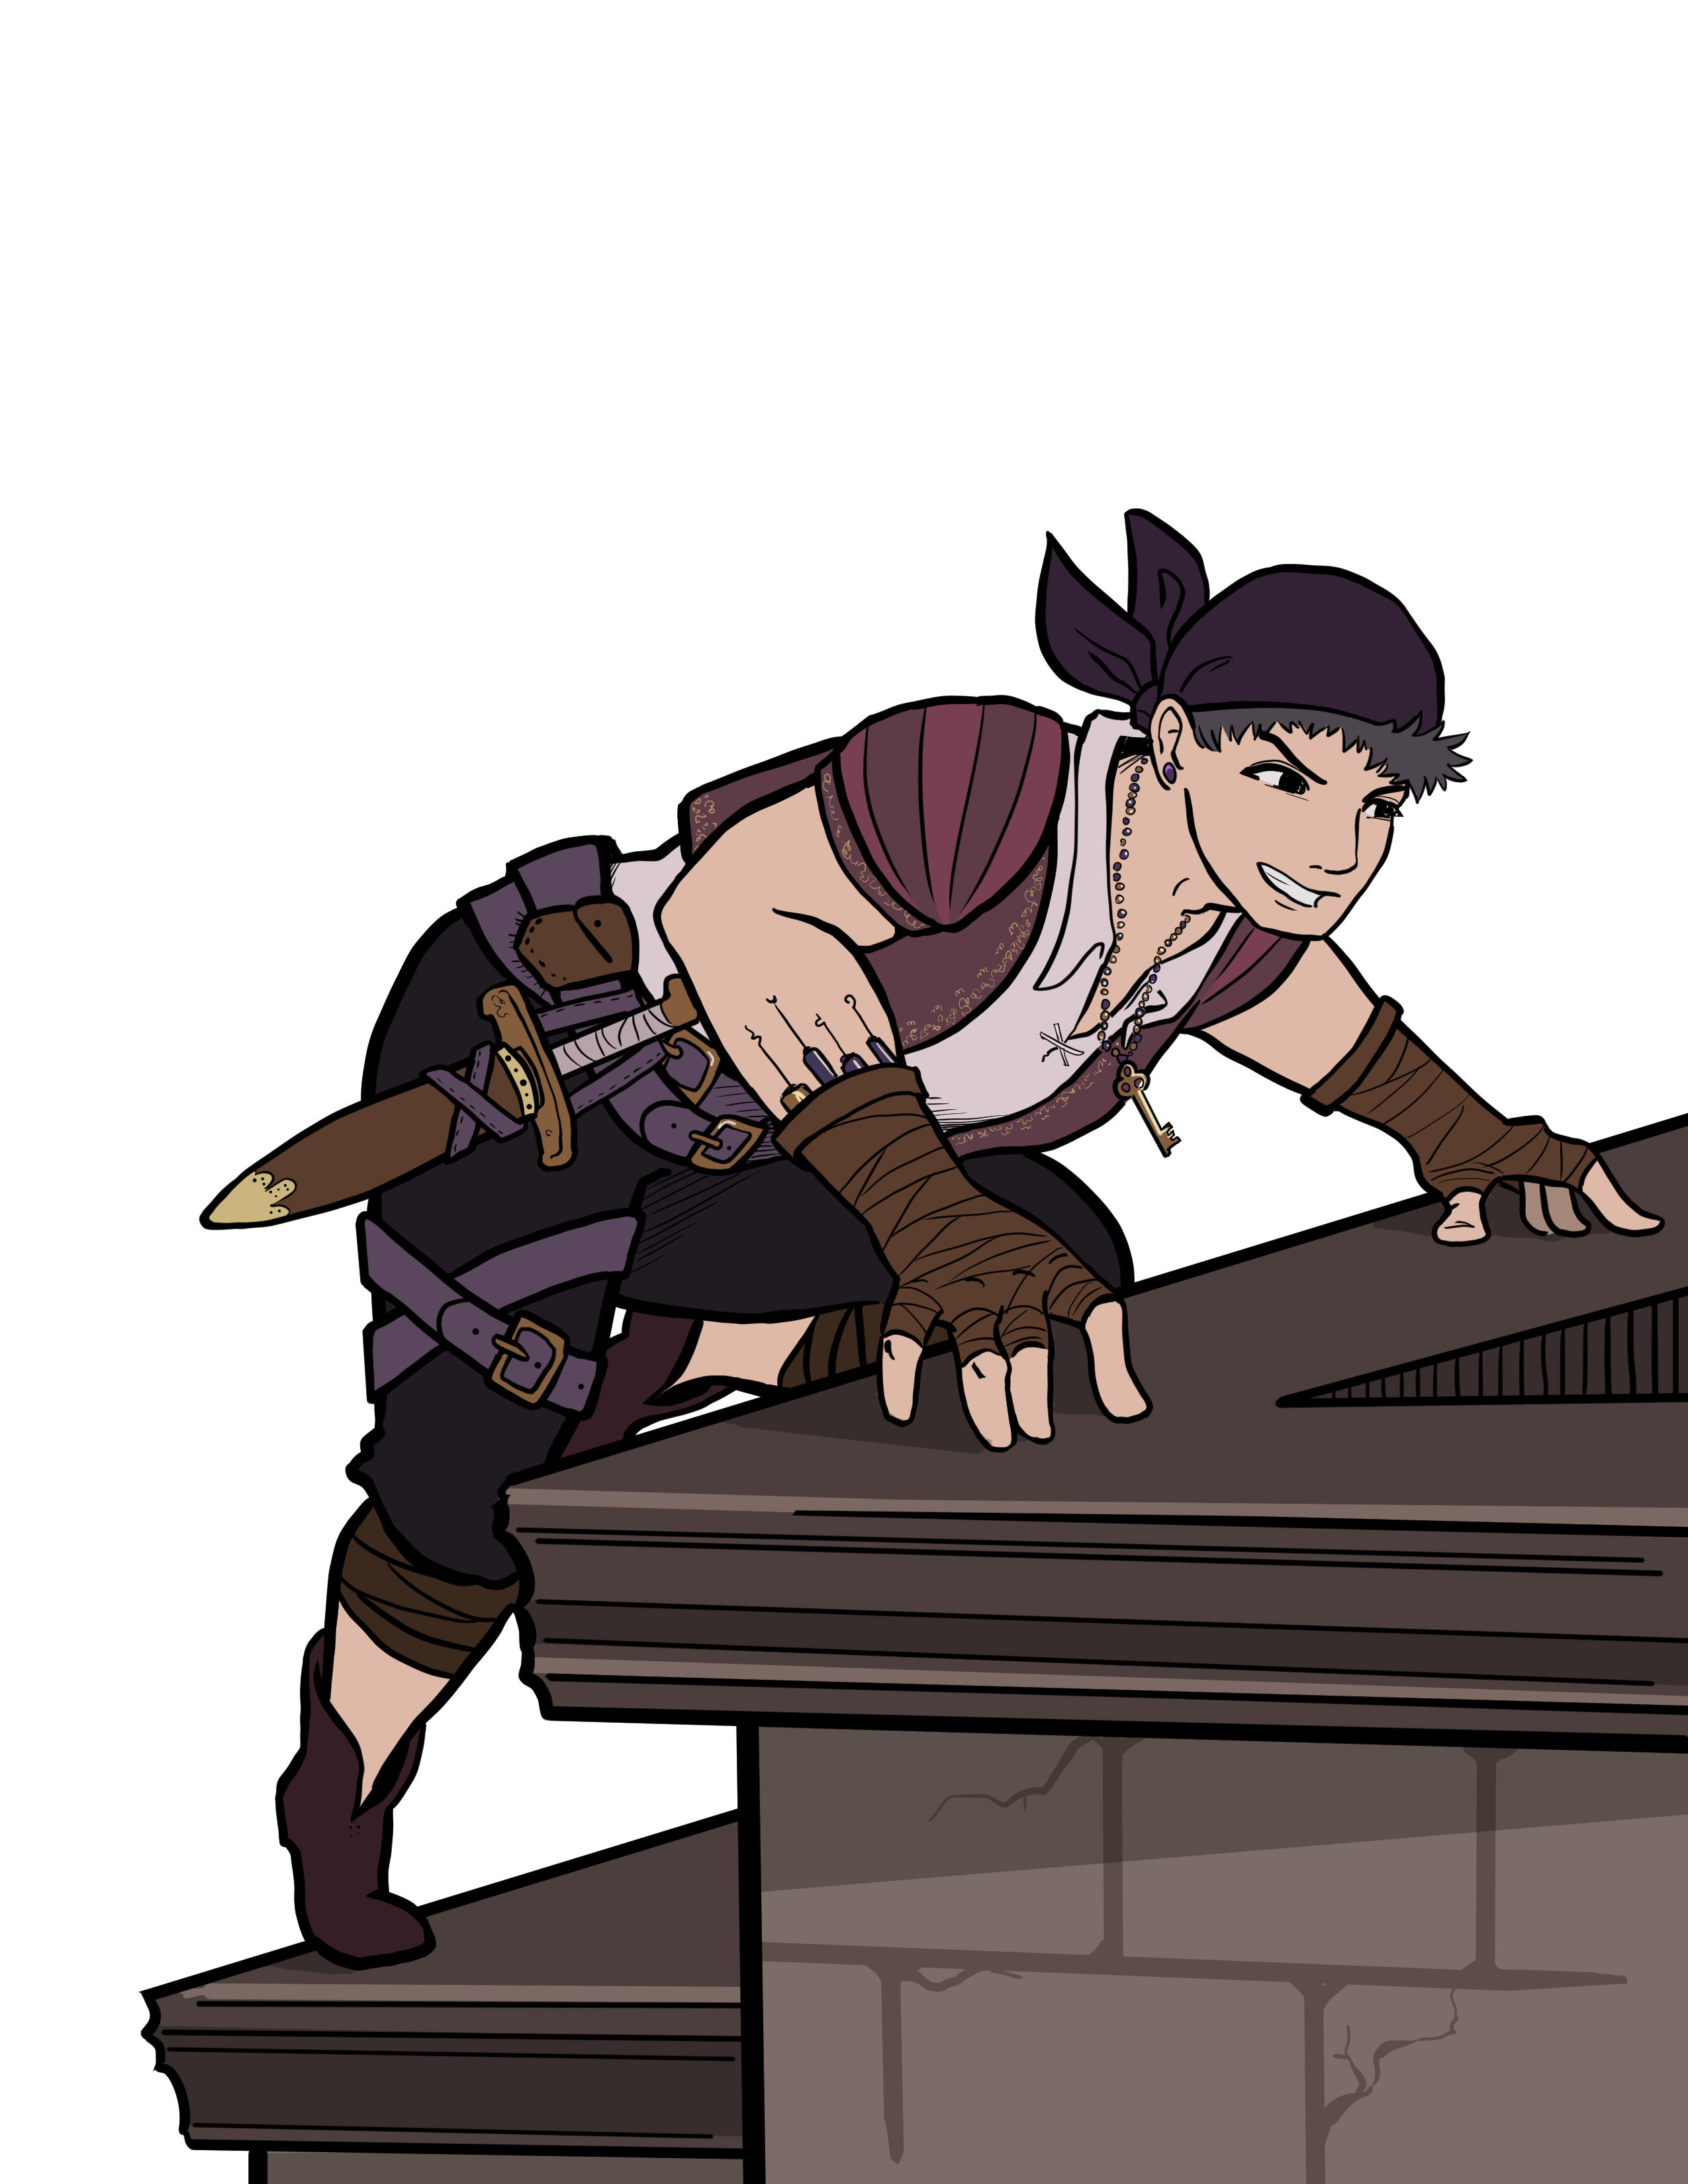
\includegraphics[width=\columnwidth]{Classes/Rogue}
Rogues are human characters who specialize in subterfuge and trickery. They come from all social classes, from bored nobles seeking excitement to wealth-seeking commoners to self-taught former street urchins.

Although they have some thieving abilities, rogue characters are not always dishonest and do not always steal. Many of them use their talents for good rather than for personal benefit, and work as scouts and adventurers. Even the most noble and honest adventuring parties often need to bypass traps and locks or to have someone who can scout ahead without being seen, and many rogues spend their adventuring careers in this type of activity and never steal a coin in their lives.

Adventuring parties find the talents of rogues extremely useful, although rogues do not make the greatest warriors so may need protecting in large fights.

\subsection{Abilities}
\textbf{Climb Walls:} Rogues are able to climb walls and other sheer surfaces. The percentage chance of success is listed in \fullref{tab:Rogue Special Abilities Progression}. The rogue’s player must roll for each 100 feet or part of 100 feet climbed, with a failure indicating that the rogue has fallen half way through the climb. See \fullref{sec:Environmental Damage} for details about falling.

In some cases a slippery or smooth surface (or a particularly rough one) may cause there to be a modifier to the rogue’s roll.

\textbf{Find Traps:}\label{sec:Find Traps} A rogue’s trained senses are able to detect the presence of traps on objects or in areas. lists the percentage chance of finding each trap in an area. The rogue does not automatically get to roll for this ability. Their player must state that the character is searching the area. The Game Master should roll the dice and inform the rogue’s player whether any traps were found.

If no traps are found the rogue will not know whether it is because there were no traps or whether they simply failed to notice them. In some cases a particularly well hidden (or badly hidden) trap may cause there to be a modifier to the rogue’s roll.

\textbf{Hear Noise:} If a rogue listens quietly at a door, window, or thin wall then they have a percentage chance of hearing faint noises that other characters would miss as listed on \fullref{tab:Rogue Special Abilities Progression}. The rogue must be in quiet conditions to use this ability—noisy chatter of other characters or fighting swamps any noises that might be heard.

The Game Master should roll for the success of this ability so that if the result is negative the rogue’s player does not know whether this was because the roll failed or because there was nothing to hear.

This ability replaces the character's normal chance of listening.

\textbf{Hide in Shadows:} A rogue is able to hide effectively providing there is cover or shadows to hide in. The percentage chance of success is listed in \fullref{tab:Rogue Special Abilities Progression}. The rogue’s player must roll for the initial hiding, and then for each round of movement, with a failure indicating that the rogue has temporarily become visible.

The Game Master should roll the dice when the rogue is hiding, so that the rogue’s player does not know whether or not their character has been spotted. If someone is watching the rogue before they start to hide, they will still be able to see the rogue regardless of the success or otherwise of this ability.

\textbf{Move Silently:}\label{sec:Move Silently} Rogues are able to move without being heard. The percentage chance of success is listed in \fullref{tab:Rogue Special Abilities Progression}. The rogue’s player must roll for each round of movement, with a failure indicating that the rogue has made a sound that others might hear. The Game Master should roll the dice when the rogue is sneaking, so that the rogue’s player does not know whether or not their character has been heard.

\textbf{Open Locks:}\label{sec:Open Locks} If a rogue is in possession of a set of lock picks, or tools that can make improvised lock picks, they can attempt to pick any lock with a percentage chance of success listed in \fullref{tab:Rogue Special Abilities Progression}. Doing so will set off any trap that the lock is armed with unless the trap has been removed or otherwise disabled. In some cases a particularly complex (or simple) lock may cause there to be a modifier to the rogue’s roll.

A rogue is only allowed one attempt to pick each lock they encounter. Should they fail then they will not be able to try to open that lock again until they have increased in level.

\textbf{Pick Pockets:} A rogue is able to pick the pockets of others in order to steal small items from them, with a base percentage chance of success listed in \fullref{tab:Rogue Special Abilities Progression}. This ability can be used to steal purses or belt pouches, or even steal a weapon from its scabbard, but cannot be used to steal anything that is being held by the target or is strapped onto the target such as a backpack or armor.

The base chance of success is reduced by 5\% for each hit dice of the target.

The rogue’s player must state the item that they wish to steal before rolling. If the rogue rolls equal to or less than their modified chance of success then they successfully steal the item. If they roll more than their modified chance of success but less than or equal to twice that chance then they are unable to steal the item but their attempted theft goes unnoticed.

If they roll more than twice their modified chance of success, or roll a 00, then not only are they unable to steal the item but they are also noticed in the attempt by the target of the theft.

\textbf{Remove Traps:} If a rogue is aware of the existence of a trap, they may try to disarm it to prevent it from being triggered. The percentage chance of this ability working successfully is listed on \fullref{tab:Rogue Special Abilities Progression}. Should this ability fail, the trap will be activated. In some cases a particularly complex (or simple) trap may cause there to be a modifier to the rogue’s roll.

A rogue may try multiple times to remove the same trap, although since the trap is activated each time the rogue tries, doing so can be a dangerous activity.

\textbf{Sneak Attack:} If a rogue is able to strike an opponent who is not aware of the rogue’s location, the rogue can add +4 to their attack roll and if the attack hits it does twice the normal damage that the attack would normally do. Should a rogue make two simultaneous attacks (because they are wielding two weapons) then both attacks get the +4 bonus and do double damage if they hit.

Simply being behind an enemy is not enough to get a sneak attack. The rogue must actually be hidden, invisible, or otherwise concealed, and their location must not be known to their target.

The sneak attack may be made with a melee attack or with a Projectile weapon at short range.

\textbf{Read Languages:} At \nth{4} level or higher, a rogue has an 80\% chance to be able to decipher any non-magical written language or code.

This only works on written text and cannot be used to understand spoken languages.

\textbf{Use Wizard Scroll:} Beginning at \nth{10} level, a rogue has a 90\% chance of being able to decipher and use any scroll containing a wizard spell.

Should this roll fail, the spell will still be used up from the scroll but will misfire.

An offensive spell will go off centered on the rogue rather than their intended target, and a non-offensive spell will simply fizzle with no effect.

\statblock{\textbf{Ability Requirements:} Dexterity 9

\textbf{Prime Requisite:} Dexterity

\textbf{Hit Dice:} 1d4

\textbf{Movement:} 40 feet

\textbf{Weapons:} Any one-handed and any missile

\textbf{Armor:} Hide Armor, Leather Armor

\textbf{Special Abilities:} Climb Walls, Find Traps, Hear Noise, Hide in Shadows, Move Silently, Open Locks, Pick Pockets, Remove Traps, Sneak Attack, Read Languages, Use Wizard Scroll}

\end{multicols*}
\begin {table}[H]
  \caption{Rogue Progression}
	\begin{tabularx}{\columnwidth}{>{\bfseries}cccM{.31in}M{.51in}M{.25in}M{.43in}M{.32in}M{.45in}Y}
    \thead{}&\thead{}&\thead{}&\thead{}&\multicolumn{5}{c}{\thead{Saving Throws}}\thead{}&\setcounter{rownum}{0}\\
    \thead{Level} & \thead{Experience} & \thead{Hit Dice} & \thead{Attack Bonus} & \thead{Death Ray/ Poison} & \thead{Magic Wands} & \thead{Paralysis/ Petrify} & \thead{Breath Weapon} & \thead{Rod/Staff/ Spell} & \thead{Special}\\
		1 & 0 & 1d4 & +1 & 13 & 14 & 13 & 16 & 15 & Climb Walls, Find Traps, Hear Noise, Hide in Shadows, Move Silently, Open Locks, Pick Pockets, Remove Traps, Sneak Attack, +4 Skill Points, +2 Weapon Feats\\
		2 & 1,200 & 2d4 & +1 & 13 & 14 & 13 & 16 & 15 & -\\
		3 & 2,400 & 3d4 & +1 & 13 & 14 & 13 & 16 & 15 & +1 Weapon Feat\\
		4 & 4,800 & 4d4 & +2 & 12 & 13 & 12 & 15 & 14 & Read Languages\\
		5 & 9,600 & 5d4 & +2 & 12 & 13 & 12 & 15 & 14 & +1 Skill Point\\
		6 & 20,000 & 6d4 & +3 & 11 & 12 & 11 & 14 & 13 & +1 Weapon Feat\\
		7 & 40,000 & 7d4 & +3 & 11 & 12 & 11 & 14 & 13 & -\\
		8 & 80,000 & 8d4 & +4 & 10 & 11 & 10 & 13 & 12 & -\\
		9 & 160,000 & 9d4 & +4 & 10 & 11 & 10 & 13 & 12 & +1 Skill Point, +1 Weapon Feat\\
		10 & 280,000 & 9d4+2 & +5 & 9 & 10 & 9 & 12 & 11 & Use Wizard Scroll\\
		11 & 400,000 & 9d4+4 & +5 & 9 & 10 & 9 & 12 & 11 & +1 Weapon Feat\\
		12 & 520,000 & 9d4+6 & +6 & 8 & 9 & 8 & 11 & 10 & -\\
		13 & 640,000 & 9d4+8 & +6 & 8 & 9 & 8 & 11 & 10 & +1 Skill Point\\
		14 & 760,000 & 9d4+10 & +7 & 7 & 8 & 7 & 10 & 9 & -\\
		15 & 880,000 & 9d4+12 & +7 & 7 & 8 & 7 & 10 & 9 & +1 Weapon Feat\\
		16 & 1,000,000 & 9d4+14 & +8 & 6 & 7 & 6 & 9 & 8 & -\\
		17 & 1,120,000 & 9d4+16 & +8 & 6 & 7 & 6 & 9 & 8 & +1 Skill Point\\
		18 & 1,240,000 & 9d4+18 & +9 & 5 & 6 & 5 & 8 & 7 & -\\
		19 & 1,360,000 & 9d4+20 & +9 & 5 & 6 & 5 & 8 & 7 & -\\
		20 & 1,480,000 & 9d4+22 & +10 & 5 & 6 & 5 & 7 & 6 & -\\
		21 & 1,600,000 & 9d4+24 & +10 & 4 & 5 & 4 & 7 & 6 & +1 Skill Point\\
		22 & 1,720,000 & 9d4+26 & +11 & 4 & 5 & 4 & 6 & 5 & -\\
		23 & 1,840,000 & 9d4+28 & +11 & 4 & 5 & 4 & 6 & 5 & +1 Weapon Feat\\
		24 & 1,960,000 & 9d4+30 & +12 & 4 & 5 & 4 & 5 & 5 & -\\
		25 & 2,080,000 & 9d4+34 & +12 & 3 & 4 & 3 & 5 & 4 & +1 Skill Point\\
		26 & 2,200,000 & 9d4+36 & +13 & 3 & 4 & 3 & 4 & 4 & -\\
		27 & 2,320,000 & 9d4+38 & +13 & 3 & 4 & 3 & 4 & 4 & -\\
		28 & 2,440,000 & 9d4+40 & +14 & 3 & 4 & 3 & 4 & 4 & -\\
		29 & 2,560,000 & 9d4+42 & +14 & 2 & 3 & 2 & 3 & 3 & +1 Skill Point\\
		30 & 2,680,000 & 9d4+44 & +15 & 2 & 3 & 2 & 3 & 2 & +1 Weapon Feat\\
		31 & 2,800,000 & 9d4+46 & +15 & 2 & 3 & 2 & 3 & 2 & -\\
		32 & 2,920,000 & 9d4+48 & +16 & 2 & 3 & 2 & 3 & 2 & -\\
		33 & 3,040,000 & 9d4+50 & +16 & 2 & 2 & 2 & 2 & 2 & +1 Skill Point\\
		34 & 3,160,000 & 9d4+52 & +17 & 2 & 2 & 2 & 2 & 2 & -\\
		35 & 3,280,000 & 9d4+54 & +17 & 2 & 2 & 2 & 2 & 2 & -\\
		36 & 3,400,000 & 9d4+56 & +18 & 2 & 2 & 2 & 2 & 2 & +1 Weapon Feat\
  \end {tabularx}
\end {table}

\begin {table}[H]
  \caption{Rogue Special Abilities Progression}
  \begin{tabularx}{\columnwidth}{>{\bfseries}YYYYYYYYYYY}\label{tab:Rogue Special Abilities Progression}
		\thead{Level} & \thead{Climb Walls} & \thead{Find Traps} & \thead{Hear Noise} & \thead{Hide in Shadows} & \thead{Move Silently} & \thead{Open Locks} & \thead{Pick Pockets} & \thead{Remove Traps} & \thead{Read Languages} & \thead{Use Magic-User Scroll}\\
		1 & 87 & 10 & 34 & 10 & 20 & 15 & 20 & 10 & - & -\\
		2 & 88 & 15 & 42 & 15 & 25 & 20 & 25 & 15 & - & -\\
		3 & 89 & 20 & 50 & 20 & 30 & 25 & 30 & 20 & - & -\\
		4 & 90 & 25 & 54 & 25 & 35 & 30 & 35 & 25 & 80 & -\\
		5 & 91 & 30 & 58 & 30 & 40 & 35 & 40 & 31 & 80 & -\\
		6 & 92 & 40 & 62 & 35 & 45 & 45 & 45 & 42 & 80 & -\\
		7 & 93 & 50 & 66 & 45 & 55 & 55 & 55 & 53 & 80 & -\\
		8 & 94 & 60 & 70 & 55 & 65 & 65 & 65 & 64 & 80 & -\\
		9 & 95 & 70 & 74 & 65 & 75 & 75 & 75 & 75 & 80 & -\\
		10 & 96 & 80 & 78 & 75 & 85 & 85 & 85 & 84 & 80 & 90\\
		11 & 97 & 90 & 82 & 85 & 95 & 95 & 95 & 93 & 80 & 90\\
		12 & 98 & 95 & 84 & 90 & 96 & 96 & 105 & 97 & 80 & 90\\
		13 & 99 & 97 & 86 & 95 & 98 & 97 & 115 & 98 & 80 & 90\\
		14 & 99 & 99 & 88 & 99 & 99 & 99 & 125 & 99 & 80 & 90\\
		15 & 100 & 100 & 90 & 100 & 100 & 100 & 129 & 100 & 80 & 90\\
		16 & 101 & 102 & 92 & 100 & 100 & 101 & 133 & 102 & 80 & 90\\
		17 & 102 & 104 & 94 & 100 & 100 & 102 & 137 & 104 & 80 & 90\\
		18 & 103 & 106 & 96 & 100 & 100 & 103 & 141 & 106 & 80 & 90\\
		19 & 104 & 108 & 98 & 100 & 100 & 104 & 144 & 108 & 80 & 90\\
		20 & 105 & 110 & 100 & 100 & 100 & 105 & 147 & 110 & 80 & 90\\
		21 & 106 & 112 & 102 & 100 & 100 & 106 & 150 & 112 & 80 & 90\\
		22 & 107 & 114 & 104 & 100 & 100 & 107 & 153 & 114 & 80 & 90\\
		23 & 108 & 116 & 106 & 100 & 100 & 108 & 156 & 116 & 80 & 90\\
		24 & 109 & 118 & 108 & 100 & 100 & 109 & 159 & 118 & 80 & 90\\
		25 & 110 & 119 & 110 & 100 & 100 & 110 & 162 & 119 & 80 & 90\\
		26 & 111 & 120 & 112 & 100 & 100 & 111 & 165 & 120 & 80 & 90\\
		27 & 112 & 121 & 114 & 100 & 100 & 112 & 168 & 121 & 80 & 90\\
		28 & 113 & 122 & 116 & 100 & 100 & 113 & 171 & 122 & 80 & 90\\
		29 & 114 & 123 & 118 & 100 & 100 & 114 & 174 & 123 & 80 & 90\\
		30 & 115 & 124 & 120 & 100 & 100 & 115 & 177 & 124 & 80 & 90\\
		31 & 116 & 125 & 122 & 100 & 100 & 116 & 180 & 125 & 80 & 90\\
		32 & 117 & 126 & 124 & 100 & 100 & 117 & 183 & 126 & 80 & 90\\
		33 & 118 & 127 & 126 & 100 & 100 & 118 & 186 & 127 & 80 & 90\\
		34 & 119 & 128 & 128 & 100 & 100 & 119 & 189 & 128 & 80 & 90\\
		35 & 119 & 129 & 129 & 100 & 100 & 120 & 192 & 129 & 80 & 90\\
		36 & 120 & 130 & 130 & 100 & 100 & 120 & 195 & 130 & 80 & 90\
  \end {tabularx}
\end {table}
\newpage
\begin{multicols*}{2}

\subsection{Subclasses}
\subsubsection{Acrobat}\index[classes]{Acrobat}
Acrobats are human characters that are skilled in acrobatics. Most acrobats make a living by performing for a circus, but some are brave enough to adventure deep into the darkest dungeons accumulating treasure worth a considerable amount more than a performer's wage.

Acrobats do not get the Find Traps, Open Locks, Pick Pockets, Remove Traps, Read Languages, and Use Wizard Scroll class abilities.

\textbf{Evade:} Acrobats can evade all psychical attacks directed at them by attackers with a lower initiative. The percentage chance of success is listed in \fullref{tab:Acrobat Special Abilities Progression}.

\textbf{Slow Fall:} If an acrobat falls, they have a chance of landing without taking any damage (see \fullref{sec:Environmental Damage}). The percentage chance of success and the max fall distance it applies to is listed in \fullref{tab:Acrobat Special Abilities Progression}. Even if successful, the acrobat will still receive fall damage for any distance beyond what is listed.

\statblock{\textbf{Ability Requirements:} Strength 15, Dexterity 16

\textbf{Bonus Skills:} Balance, Jumping}

\begin {table}[H]
  \caption{Acrobat Special Abilities Progression}\label{tab:Acrobat Special Abilities Progression}
  \begin{tabularx}{\columnwidth}{>{\bfseries}YYY}
		\thead{Level} & \thead{Evade} & \thead{Slow Fall}\\
		1 & 10 & 25/10’\\
		2 & 15 & 50/10’\\
		3 & 20 & 75/10’\\
		4 & 25 & 25/20’\\
		5 & 30 & 50/20’\\
		6 & 35 & 75/20’\\
		7 & 40 & 25/30’\\
		8 & 45 & 50/30’\\
		9 & 50 & 75/30’\\
		10 & 52 & 20/40’\\
		11 & 54 & 40/40’\\
		12 & 56 & 60/40’\\
		13 & 60 & 80/40’\\
		14 & 60 & 20/50’\\
		15 & 60 & 40/50’\\
		16 & 60 & 60/50’\\
		17 & 60 & 80/50’\\
		18 & 60 & 20/60’\\
		19 & 60 & 40/60’\\
		20 & 60 & 60/60’\\
		21 & 60 & 80/60’\\
		22 & 60 & 15/70’\\
		23 & 60 & 30/70’\\
		24 & 60 & 45/70’\\
		25 & 60 & 60/70’\\
		26 & 60 & 75/70’\\
		27 & 60 & 15/80’\\
		28 & 60 & 30/80’\\
		29 & 60 & 45/80’\\
		30 & 60 & 60/80’\\
		31 & 60 & 75/80’\\
		32 & 60 & 15/90’\\
		33 & 60 & 30/90’\\
		34 & 60 & 45/90’\\
		35 & 60 & 60/90’\\
		36 & 60 & 75/90’\
  \end {tabularx}
\end {table}

\subsubsection{Assassin}\index[classes]{Assassin}
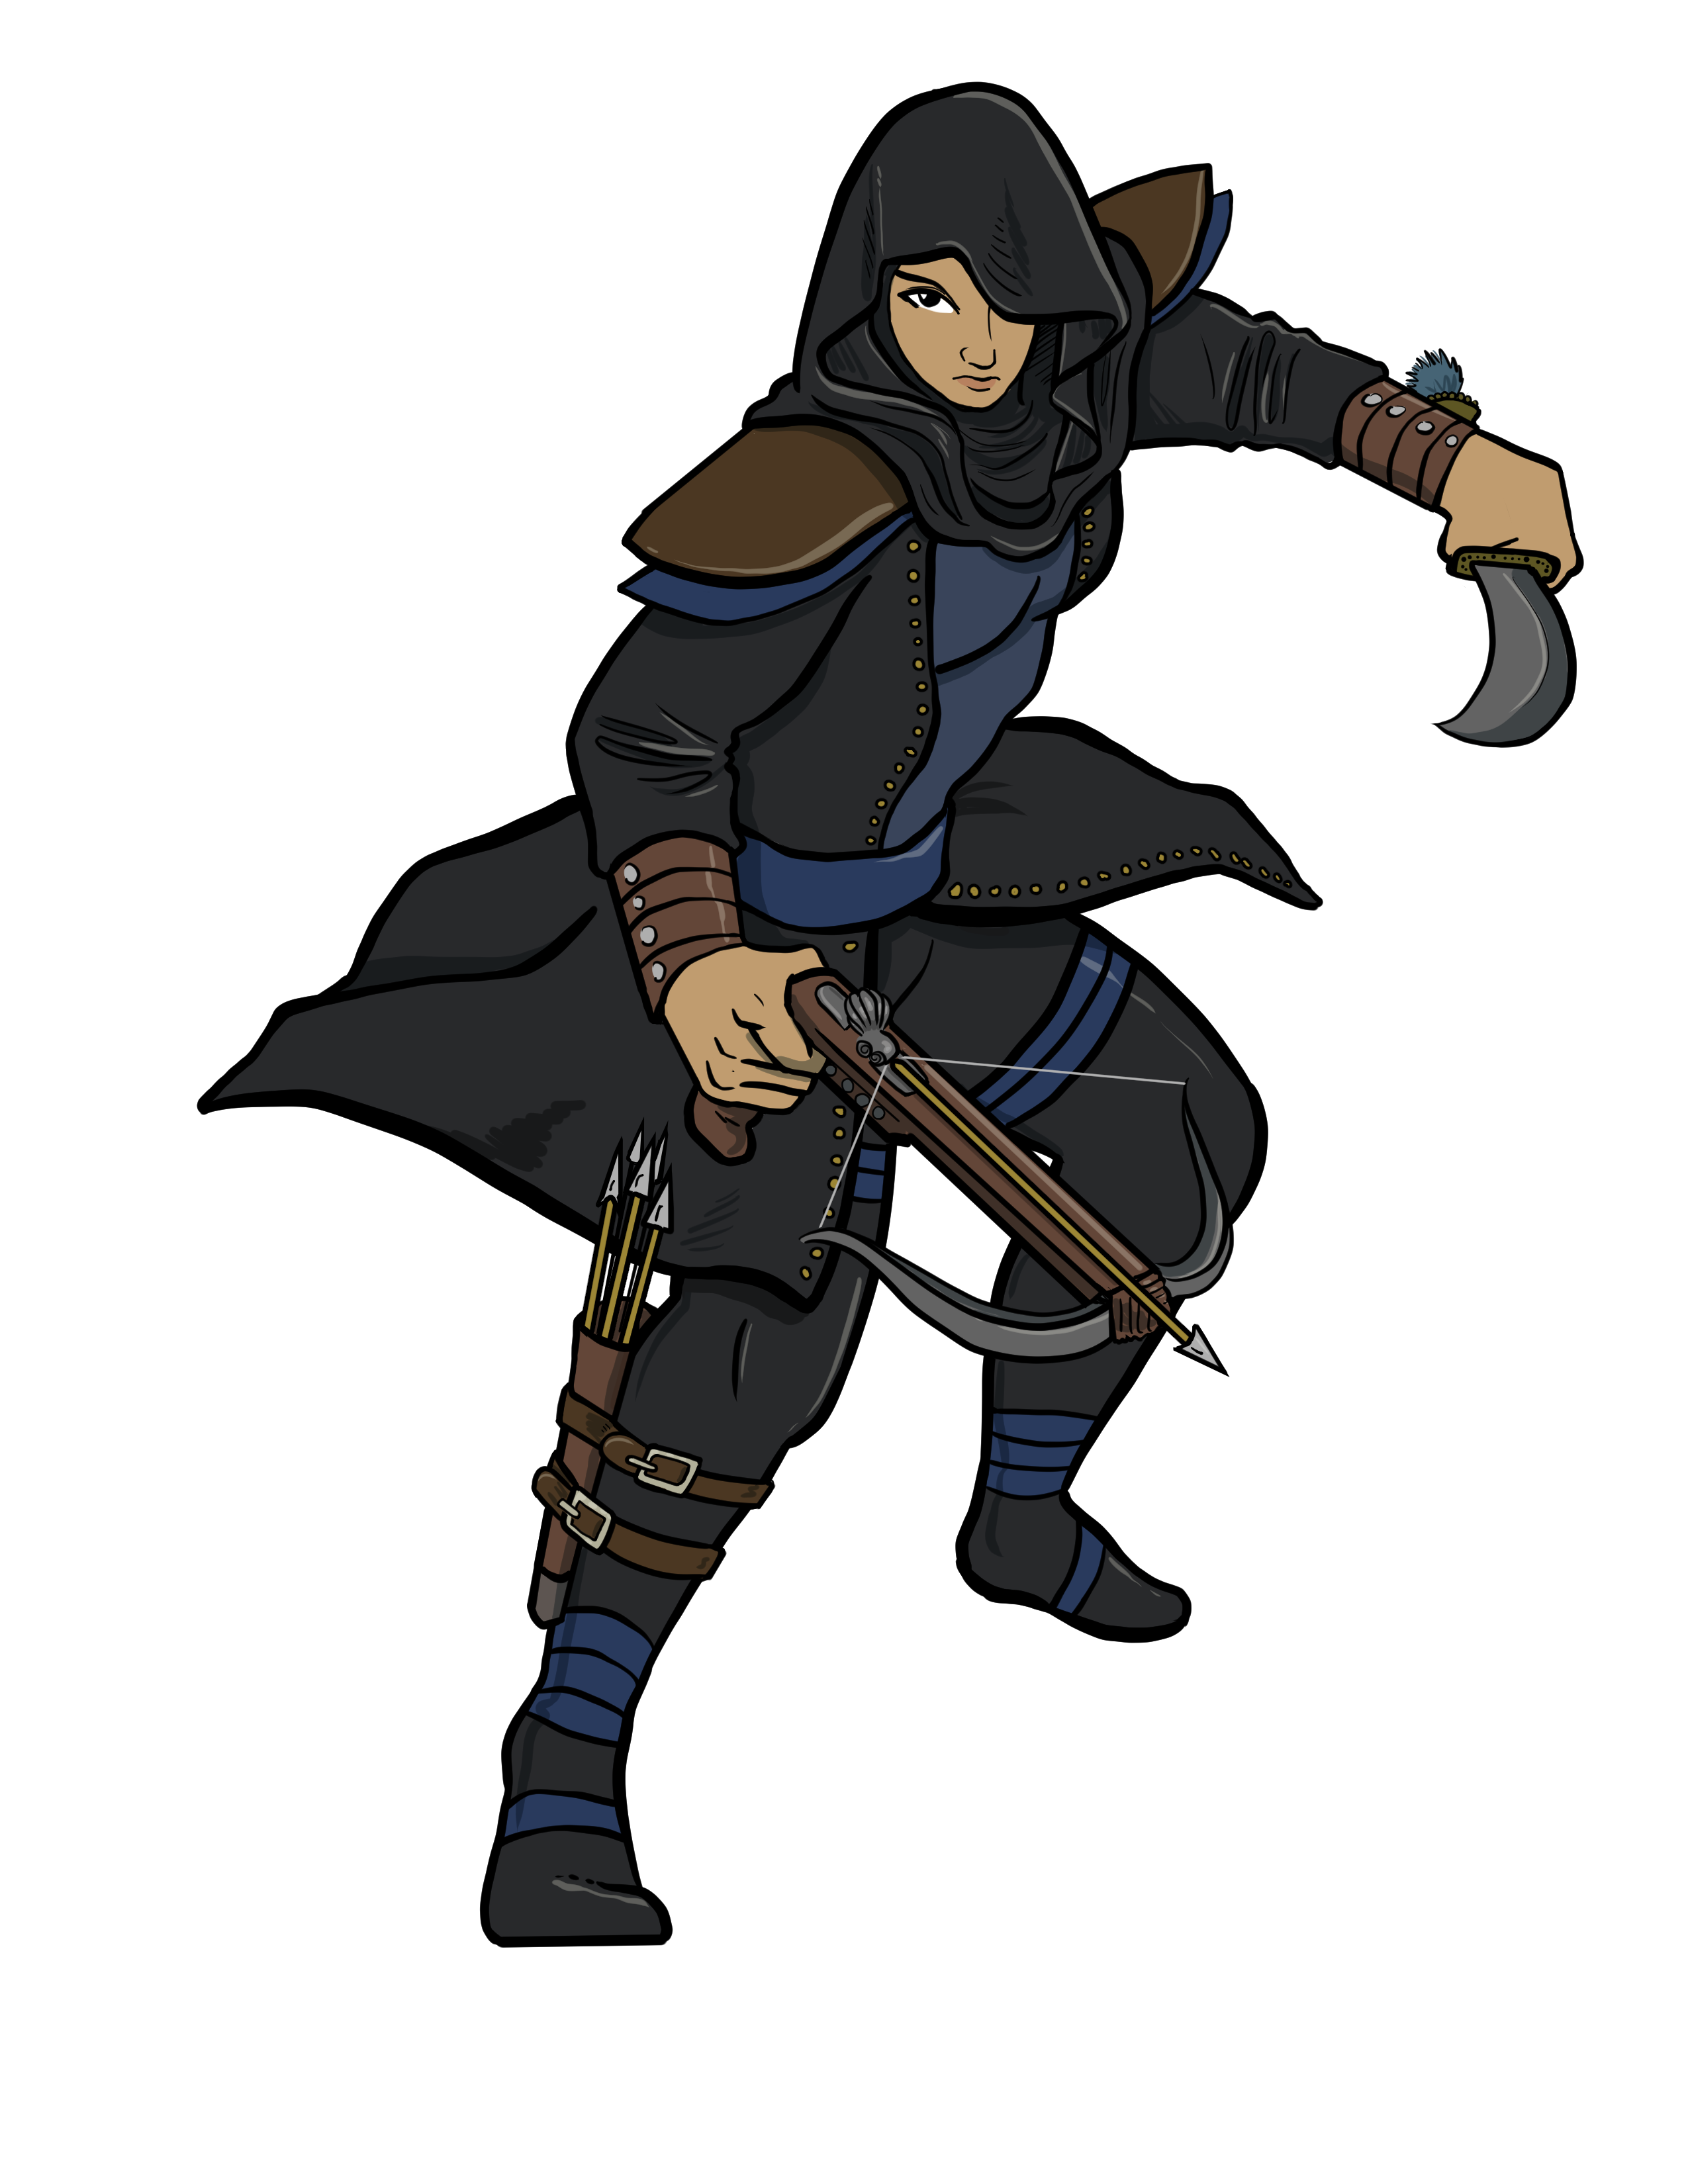
\includegraphics[width=\columnwidth]{Classes/Assassin}
Assassins are rogues that murder for hire. Utilizing their many skills, assassins will murder anyone as long as there is money to be made. It has been known for an assassin to even slit his own mother’s throat for a silver piece.

Assassins do not get the Open Locks, Pick Pockets, Read Languages, and Use Wizard Scroll class abilities.

\textbf{Assassinate:} With careful preparations and a successful surprise roll (see \fullref{sec:Surprise}, 1-3 instead of 1-2) an assassin can kill a target with a single attack. Preparations may include disguise, moving silently, hiding, or whatever else the Game Master deems appropriate for the situation.

No hit roll is required to assassinate a target; instead the chance of success is 50\%, modified by the difference of Hit Dice. For every hit die higher the target is than the assassin a -5\% is applied, for every hit die lower a +5\% is applied.

If all the requirements are met the target is slain, otherwise the attack becomes a normal attack.

\statblock{\textbf{Ability Requirements:} Strength 12, Dexterity 12, Intelligence 12

\textbf{Bonus Skills:} Disguise}

\subsubsection{Bard}\index[classes]{Bard}
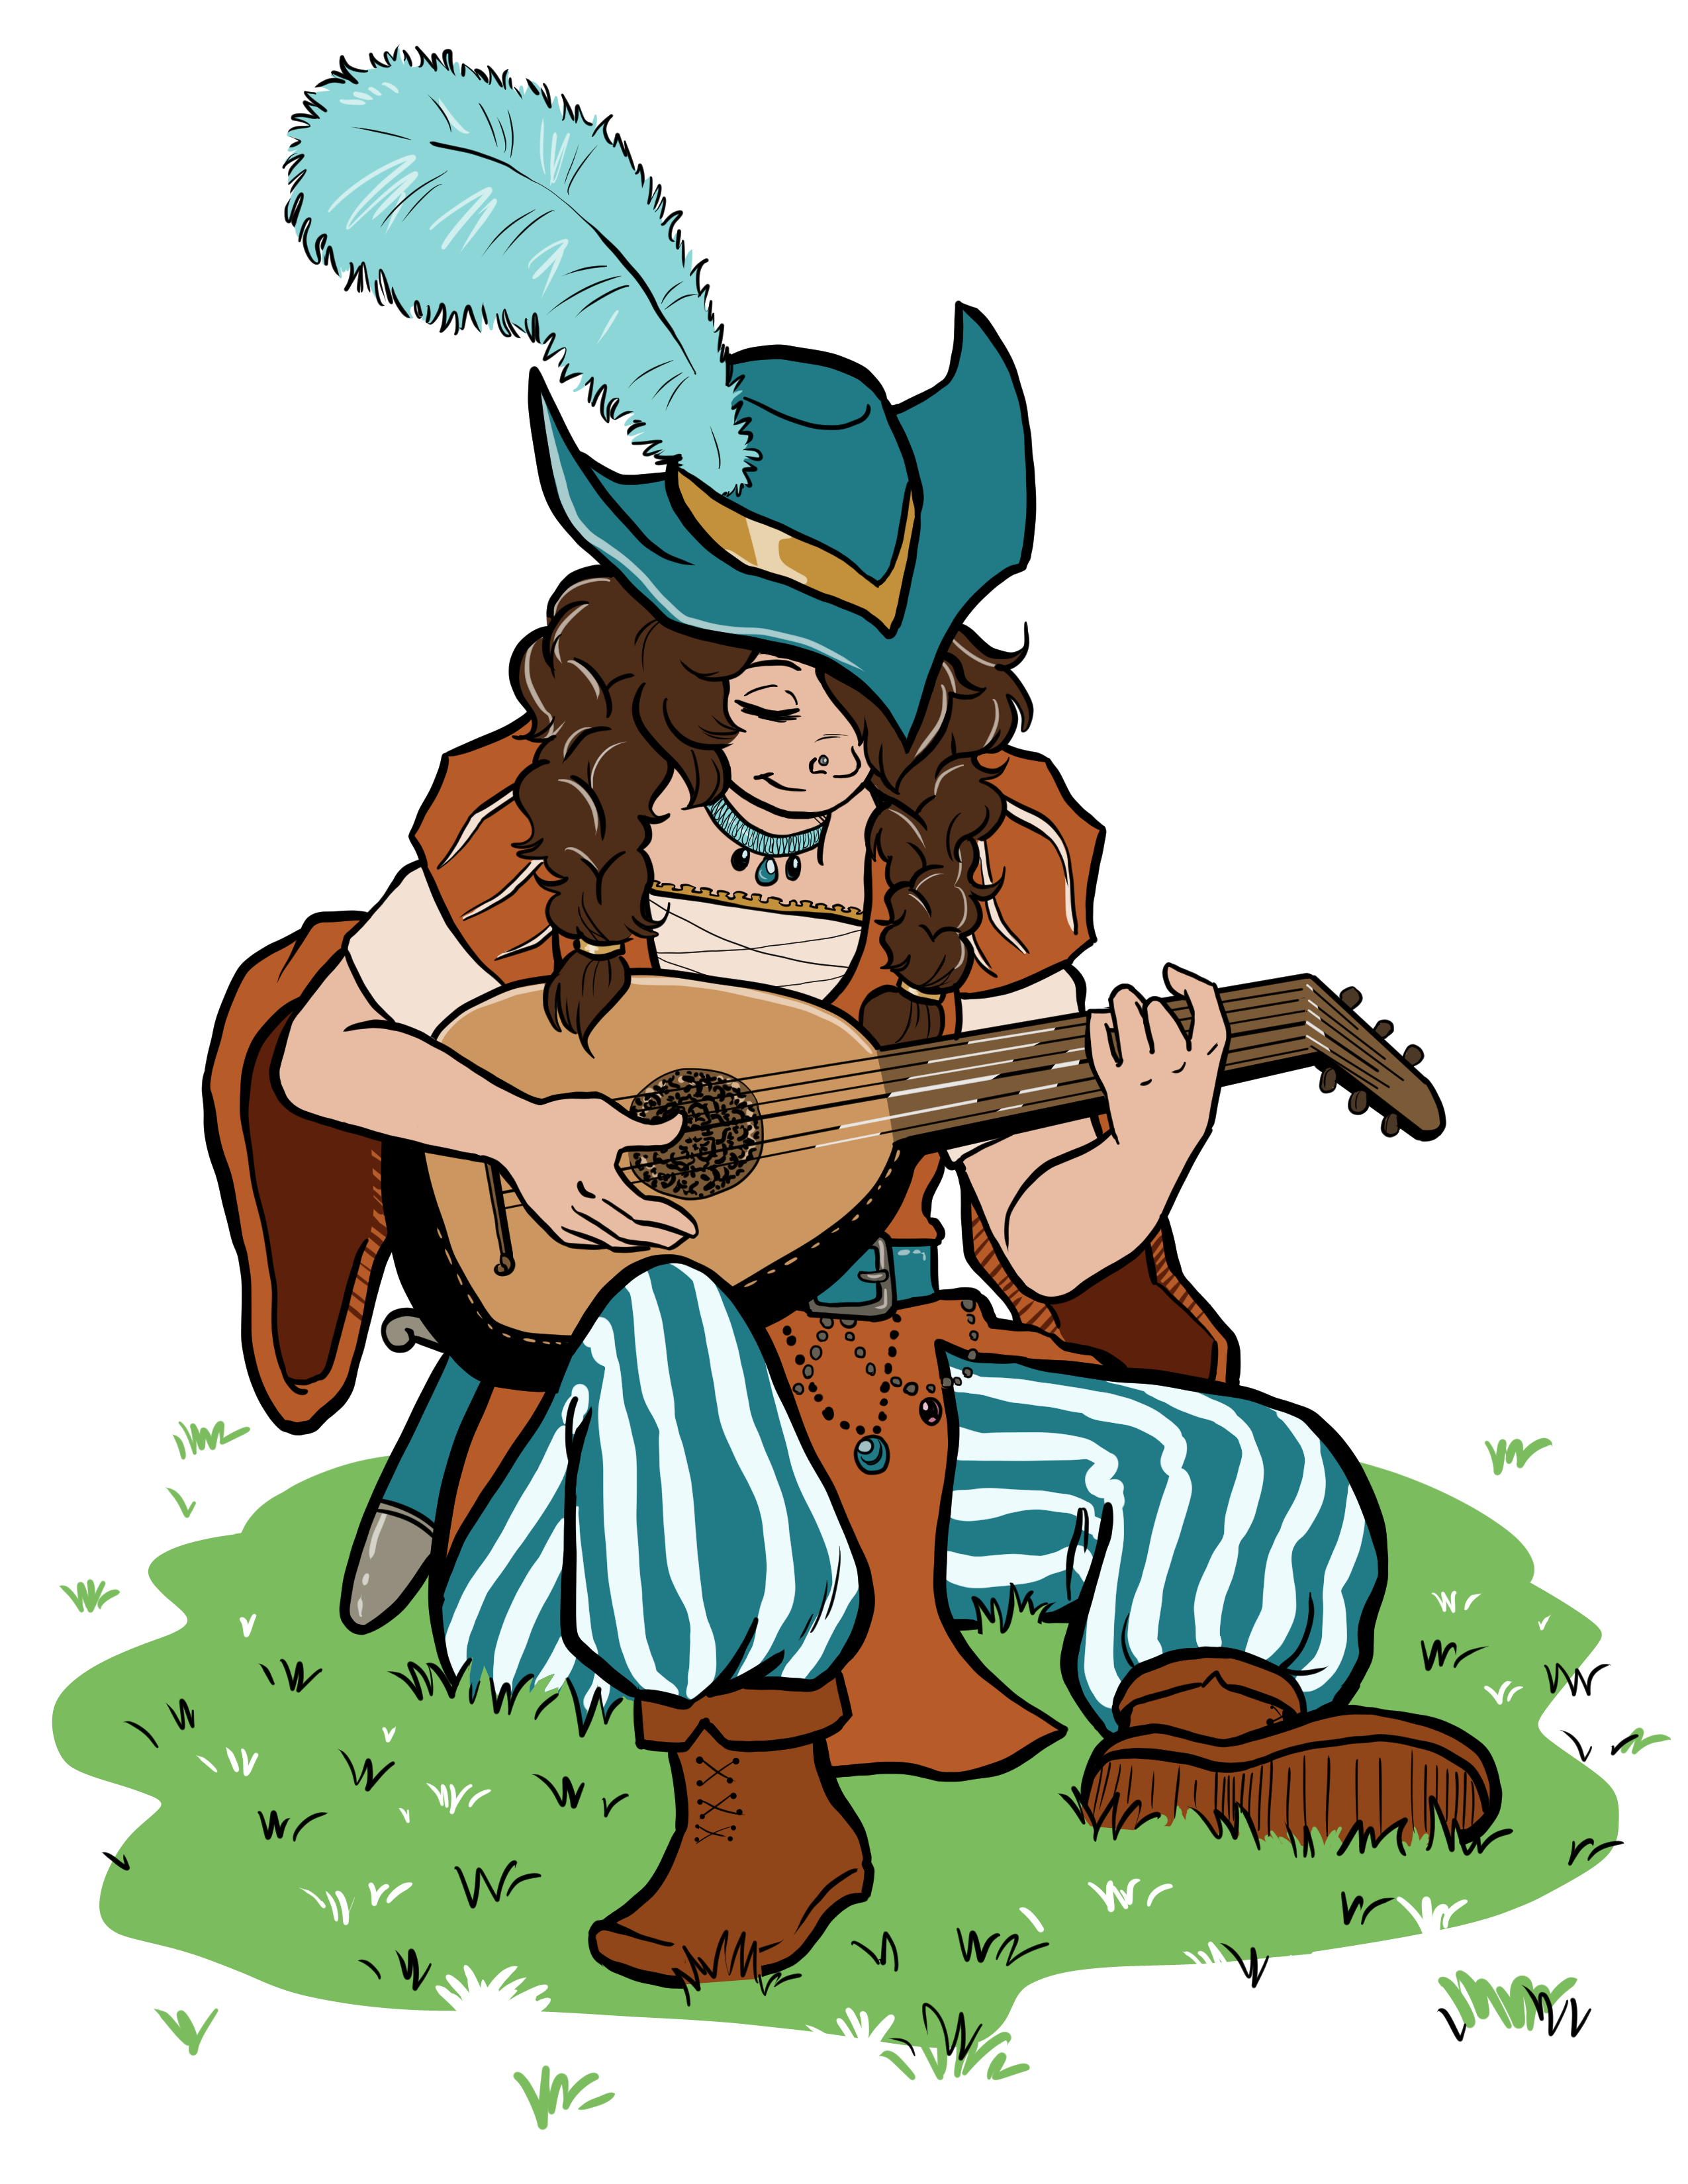
\includegraphics[width=\columnwidth]{Classes/Bard}
Bards are rogues who specialize in entertainment. They travel the world singing, playing music, reciting poems, and telling tall tales. Bards do so with such aptitude that their performance may affect listeners in almost a magical way.

Bards do not get the Pick Pockets and Sneak Attack class abilities.

\textbf{Arcane Performance:} Beginning at \nth{3} level, a bard can cause a variety of effects to his listeners by singing, playing an instrument, or reciting poetry for three rounds. A bard can affect a number of levels or hit dice equal to one-third his level (rounded down).

A successful skill check is required for the bard’s chosen performance for the effect to succeed (except for the charm effect). If the bard is interrupted or wounded the effect ends.

The effects a bard can cause with arcane performance are as followed:

\textit{Charm:} This effect functions identically to the \nth{1} level wizard spell \iref[spell:Charm Person]{Charm Person}. The victims gets a saving throw vs. spells to avoid the effect. If the bard’s skill check fails, the effect can still succeed, but the victims get a +3 bonus to their saving throw.

At \nth{9} level, this effect extends to non-undead monsters as the \nth{4} level wizard spell \iref[spell:Charm Monster]{Charm Monster}.

At \nth{15} level, this effect extends to plants as the \nth{7} level wizard spell \iref[spell:Charm Plant]{Charm Plant}.

\textit{Demoralize:} This effect diminishes the target’s morale, causing either a -2 to their morale or a -1 to hit. The targets get no saving throw to avoid the effect.

\textit{Exalt:} This effect enhances the target’s moral, granting either a +2 to their morale or a +1 to hit.

\textit{Profit:} All currency-using creatures within earshot will tip the bard for his performance. The amount tipped for each listener is 1 copper piece plus another for every point the bard succeeded their check by.

\subsubsection{Swashbuckler}\index[classes]{Swashbuckler}
Swashbucklers are acrobatic swordsmen who thirst for adventure. They are sophisticated, witty, and highly charismatic. Swashbucklers tend to dwell in cities, but will pursue adventure no matter where it leads them.

Swashbucklers do not get the Pick Pockets and Sneak Attack class abilities.

\textbf{Charisma Bonus:} Swashbucklers receive a +1 bonus to their charisma ability score. The score may not be raised to more than 18 in this way.

\textbf{Dodge:} A swashbuckler who has won initiative may dodge one melee attack. The percentage chance of success is equal to their Move Silently percentage, but may not exceed 90\%.

If the swashbuckler declares no attacks, they may try to dodge all melee attacks this round. Each attack requires a separate roll.

\textbf{Required Skills:} Balance, Bluff, Etiquette, Jumping

\section{Wizard}\index[classes]{Wizard}\label{class:Wizard}
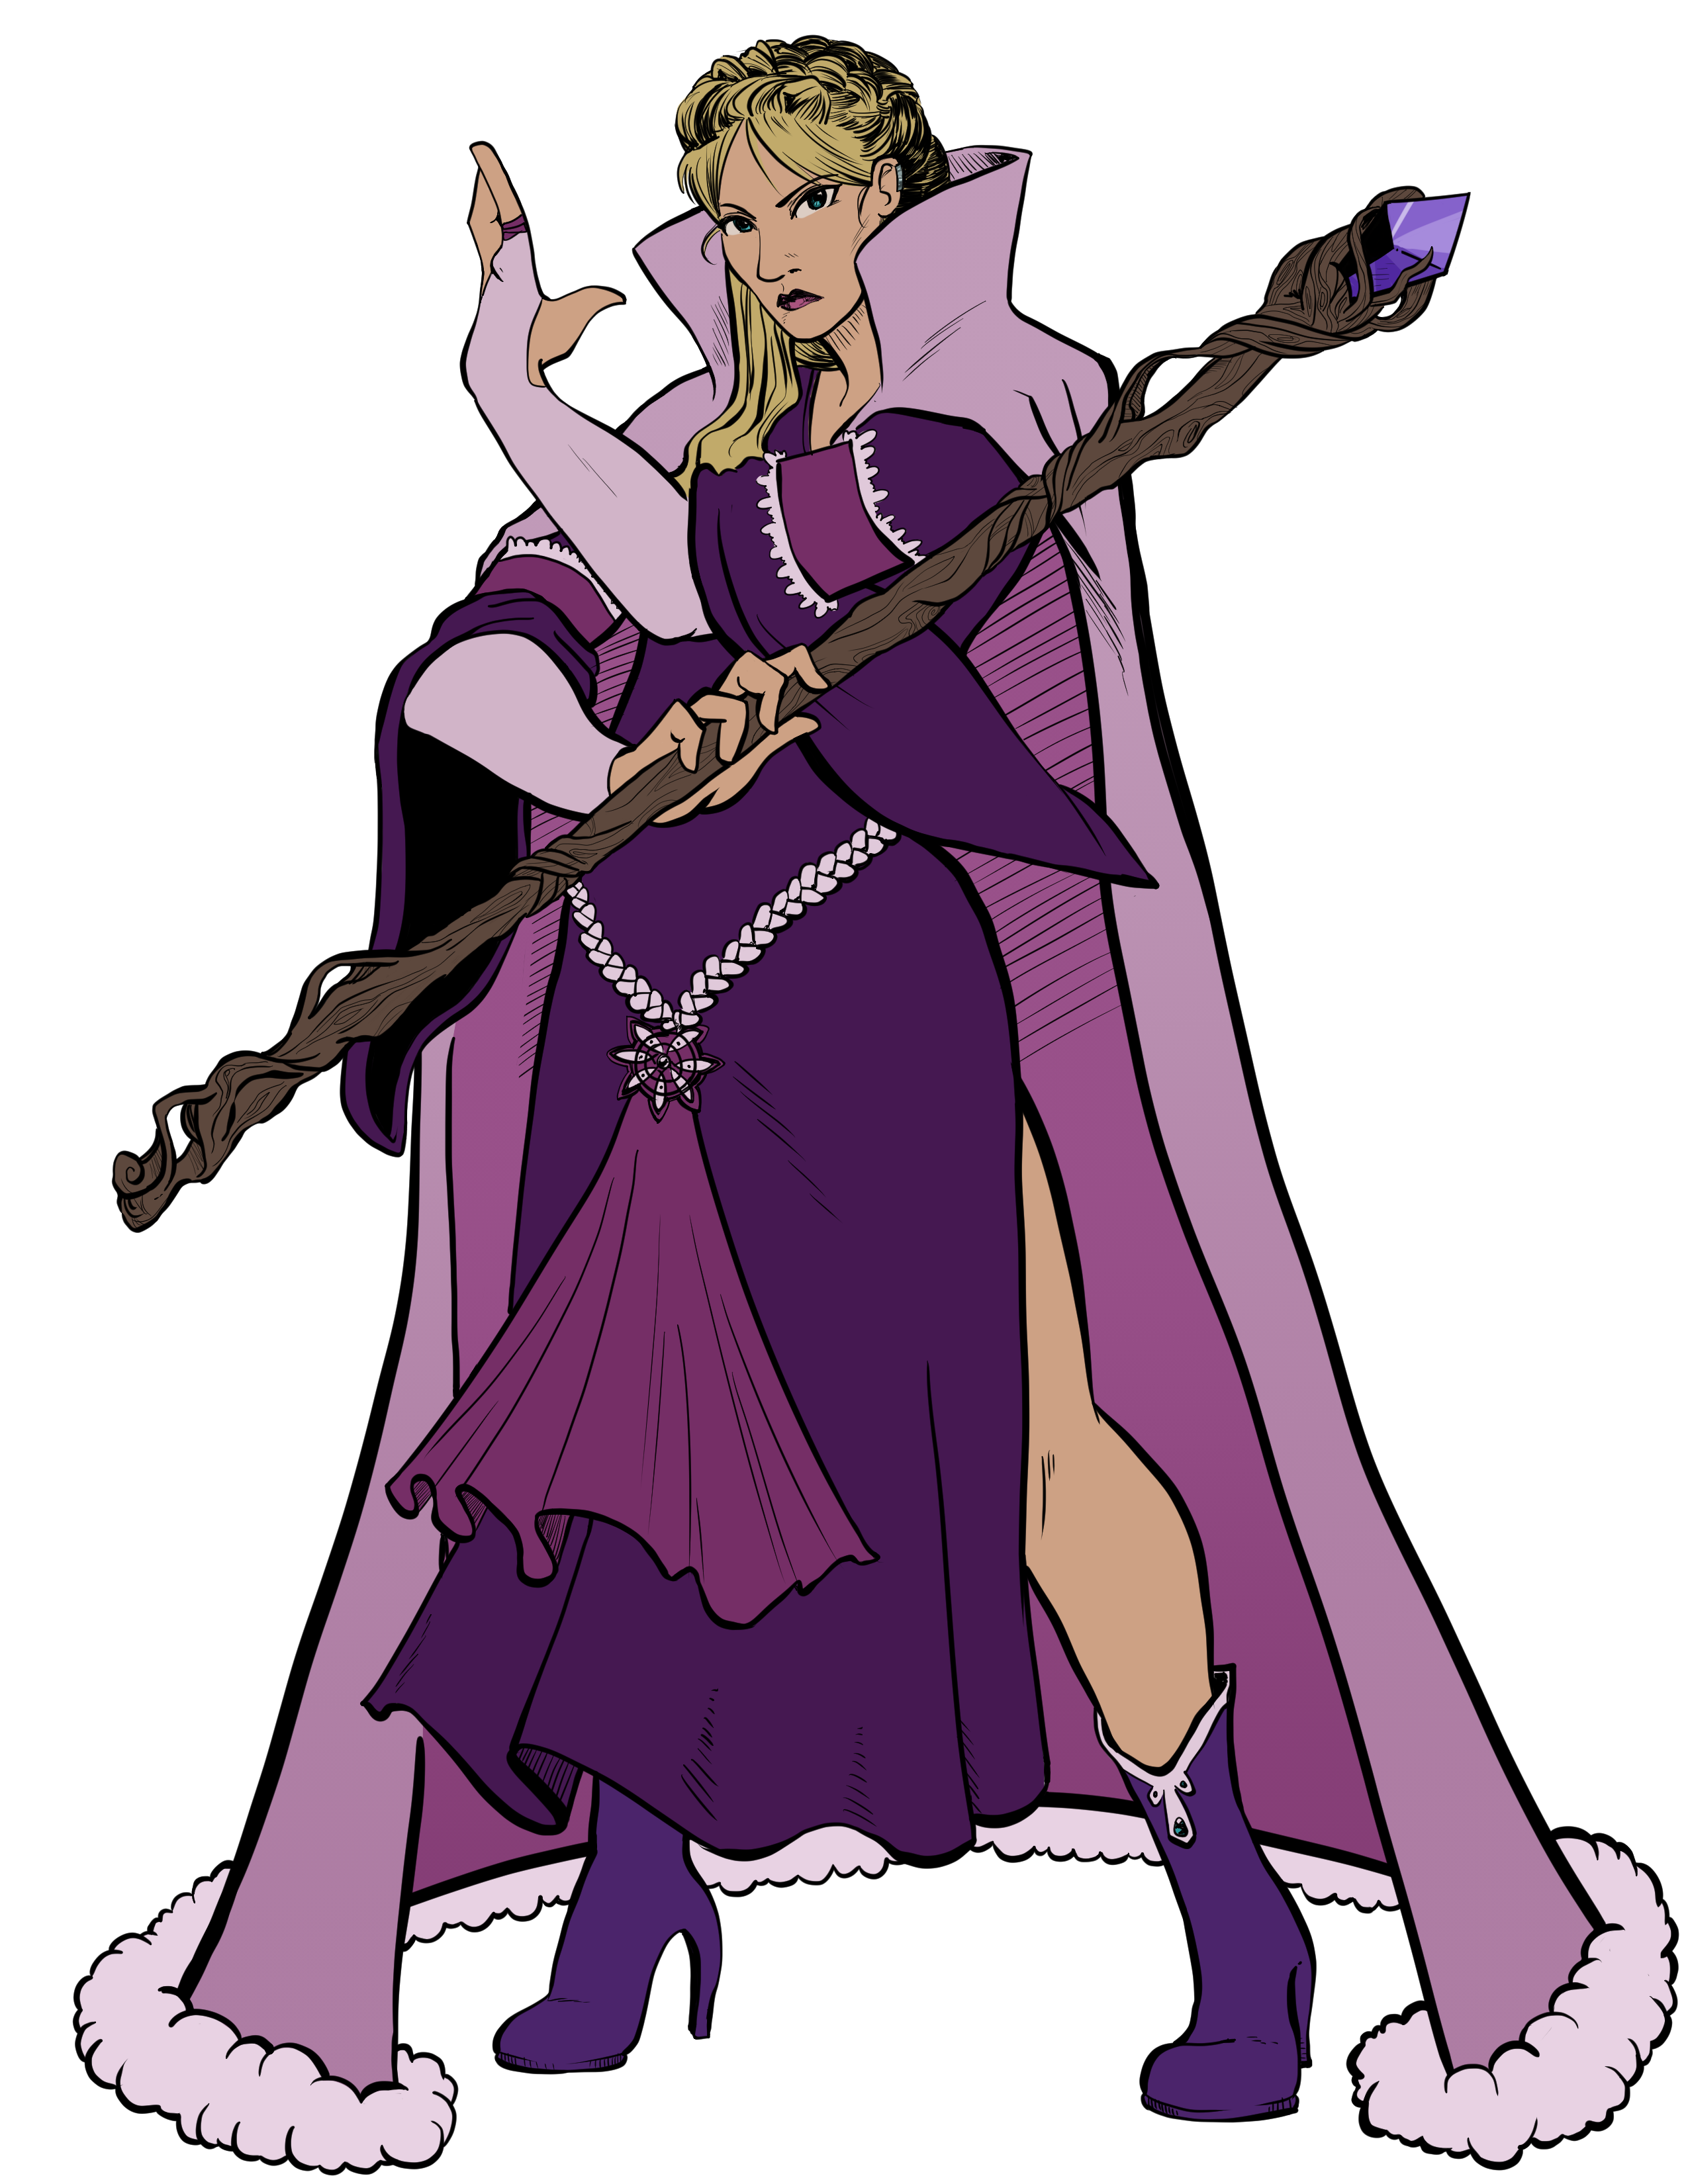
\includegraphics[width=\columnwidth]{Classes/Wizard}
Wizards are human characters who have studied the arcane arts and who are able to cast magical spells.

Unlike the inherently magical elves, magic does not come easily to humans, and prospective wizards must study for years before they are able to master it. In some larger cities such studying is done in a university, but in more rural areas with fewer resources and fewer people it is more likely to be a master/apprentice system. Unfortunately either kind of study leaves little time for other pursuits and this means that wizards tend to be somewhat lacking in more physical traits and skills.

In an adventuring party, a wizard makes excellent artillery with a wide range of offensive spells; but must be protected by other characters as they are physically weak. At low levels, the small number of spells that a wizard has can make them almost a liability to their party—but wise parties look after their wizards since should they survive to high level they will begin to wield awesome destructive power.

\subsection{Abilities}
\textbf{Spells:} Wizards can cast wizard spells. See \fullref{sec:Spell Descriptions} for detailed descriptions of these spells.

Providing a wizard has had a good night’s sleep (8 hours), they can spend an hour studying their spell book after waking up in order to gain spells for the day as indicated on \fullref{tab:Wizard Spells per Day by Spell Level}.

A \nth{1} level wizard starts with only two spells in their spell book, and must acquire more during their adventures. Wizards may prepare any spell from their book in either the normal or the reversed form (if the spell has a reversed form), but may not prepare spells from someone else’s book or from a scroll; not even by using a \iref[spell:Read Magic]{Read Magic} spell.

Each prepared spell can be cast once during the day, and if a wizard wishes to cast a spell more than once then they must prepare the spell more than once, taking up multiple spell slots of the spell’s level. Some magic user spells are reversible. These spells can be reversed in order to have an effect opposite to the normal effect of the spell. A wizard chooses whether or not to reverse the spell at the time of preparation, not at the time of casting.

A beginning wizard starts with a spell book given to them by their master, and this spell book will contain the spell \iref[spell:Read Magic]{Read Magic} and one other \nth{1} level spell of the player’s choice. This spell book is a gift from the character’s master and does not need to be paid for.

See \fullref{chap:Spells and Spellcasting} for more information on spells and spellcasting.

\statblock{\textbf{Ability Requirements:} Intelligence 9

\textbf{Prime Requisite:} Intelligence

\textbf{Hit Dice:} 1d4

\textbf{Movement:} 30 feet

\textbf{Weapons:} Blowgun, dagger, pistol, net, sling, staff, whip

\textbf{Armor:} None

\textbf{Special Abilities:} Spells}

\end{multicols*}
\begin {table}[H]
  \caption{Wizard Progression}
	\begin{tabularx}{\columnwidth}{>{\bfseries}cccM{.31in}M{.51in}M{.25in}M{.43in}M{.32in}M{.45in}Y}
    \thead{}&\thead{}&\thead{}&\thead{}&\multicolumn{5}{c}{\thead{Saving Throws}}\thead{}&\setcounter{rownum}{0}\\
    \thead{Level} & \thead{Experience} & \thead{Hit Dice} & \thead{Attack Bonus} & \thead{Death Ray/ Poison} & \thead{Magic Wands} & \thead{Paralysis/ Petrify} & \thead{Breath Weapon} & \thead{Rod/Staff/ Spell} & \thead{Special}\\
		1 & 0 & 1d4 & +1 & 13 & 14 & 13 & 16 & 15 & Spells, +4 Skill Points, +2 Weapon Feats\\
		2 & 2,500 & 2d4 & +1 & 13 & 14 & 13 & 16 & 15 & -\\
		3 & 5,000 & 3d4 & +1 & 13 & 14 & 13 & 16 & 15 & +1 Weapon Feat\\
		4 & 10,000 & 4d4 & +1 & 13 & 14 & 13 & 16 & 14 & -\\
		5 & 20,000 & 5d4 & +2 & 12 & 13 & 12 & 15 & 14 & +1 Skill Point\\
		6 & 40,000 & 6d4 & +2 & 12 & 13 & 12 & 15 & 13 & +1 Weapon Feat\\
		7 & 80,000 & 7d4 & +3 & 11 & 12 & 11 & 14 & 13 & -\\
		8 & 150,000 & 8d4 & +3 & 11 & 12 & 11 & 14 & 12 & -\\
		9 & 300,000 & 9d4 & +3 & 11 & 12 & 11 & 14 & 11 & +1 Skill Point, +1 Weapon Feat\\
		10 & 450,000 & 9d4+1 & +4 & 10 & 11 & 10 & 13 & 11 & -\\
		11 & 600,000 & 9d4+2 & +4 & 10 & 11 & 10 & 13 & 10 & +1 Weapon Feat\\
		12 & 750,000 & 9d4+3 & +5 & 9 & 10 & 9 & 12 & 10 & -\\
		13 & 900,000 & 9d4+4 & +5 & 9 & 10 & 9 & 12 & 9 & +1 Skill Point\\
		14 & 1,050,000 & 9d4+5 & +5 & 9 & 10 & 9 & 12 & 8 & -\\
		15 & 1,200,000 & 9d4+6 & +6 & 8 & 9 & 8 & 11 & 8 & +1 Weapon Feat\\
		16 & 1,350,000 & 9d4+7 & +6 & 8 & 9 & 8 & 11 & 7 & -\\
		17 & 1,500,000 & 9d4+8 & +7 & 7 & 8 & 7 & 10 & 7 & +1 Skill Point\\
		18 & 1,650,000 & 9d4+9 & +7 & 7 & 8 & 7 & 10 & 6 & -\\
		19 & 1,800,000 & 9d4+10 & +7 & 7 & 8 & 7 & 10 & 6 & -\\
		20 & 1,950,000 & 9d4+11 & +8 & 6 & 7 & 6 & 9 & 5 & -\\
		21 & 2,100,000 & 9d4+12 & +8 & 6 & 7 & 6 & 9 & 5 & +1 Skill Point\\
		22 & 2,250,000 & 9d4+13 & +9 & 5 & 6 & 5 & 8 & 4 & -\\
		23 & 2,400,000 & 9d4+14 & +9 & 5 & 6 & 5 & 8 & 4 & +1 Weapon Feat\\
		24 & 2,550,000 & 9d4+15 & +9 & 5 & 5 & 5 & 7 & 4 & -\\
		25 & 2,700,000 & 9d4+16 & +10 & 4 & 5 & 4 & 7 & 3 & +1 Skill Point\\
		26 & 2,850,000 & 9d4+17 & +10 & 4 & 4 & 4 & 6 & 3 & -\\
		27 & 3,000,000 & 9d4+18 & +11 & 4 & 4 & 4 & 6 & 3 & -\\
		28 & 3,150,000 & 9d4+19 & +11 & 4 & 4 & 4 & 5 & 3 & -\\
		29 & 3,300,000 & 9d4+20 & +11 & 3 & 3 & 3 & 5 & 2 & +1 Skill Point\\
		30 & 3,450,000 & 9d4+21 & +12 & 3 & 3 & 3 & 4 & 2 & +1 Weapon Feat\\
		31 & 3,600,000 & 9d4+22 & +12 & 3 & 3 & 3 & 4 & 2 & -\\
		32 & 3,750,000 & 9d4+23 & +13 & 3 & 3 & 3 & 3 & 2 & -\\
		33 & 3,900,000 & 9d4+24 & +13 & 2 & 2 & 2 & 3 & 2 & +1 Skill Point\\
		34 & 4,050,000 & 9d4+25 & +13 & 2 & 2 & 2 & 2 & 2 & -\\
		35 & 4,200,000 & 9d4+26 & +14 & 2 & 2 & 2 & 2 & 2 & -\\
		36 & 4,350,000 & 9d4+27 & +15 & 2 & 2 & 2 & 2 & 2 & +1 Weapon Feat\
  \end {tabularx}
\end {table}
\newpage
\begin{multicols*}{2}

\begin {table}[H]
  \caption{Wizard Spells per Day by Spell Level}\label{tab:Wizard Spells per Day by Spell Level}
  \begin{tabularx}{\columnwidth}{>{\bfseries}YYYYYYYYYY}
		\thead{} & \multicolumn{9}{c}{\thead{Spell Level}}\\
		\thead{Level} & \thead{1} & \thead{2} & \thead{3} & \thead{4} & \thead{5} & \thead{6} & \thead{7} & \thead{8} & \thead{9}\\
		1 & 1 & - & - & - & - & - & - & - & -\\
		2 & 2 & - & - & - & - & - & - & - & -\\
		3 & 2 & 1 & - & - & - & - & - & - & -\\
		4 & 2 & 2 & - & - & - & - & - & - & -\\
		5 & 2 & 2 & 1 & - & - & - & - & - & -\\
		6 & 3 & 2 & 2 & - & - & - & - & - & -\\
		7 & 3 & 2 & 2 & 1 & - & - & - & - & -\\
		8 & 3 & 3 & 2 & 2 & - & - & - & - & -\\
		9 & 3 & 3 & 2 & 2 & 1 & - & - & - & -\\
		10 & 4 & 3 & 3 & 2 & 2 & - & - & - & -\\
		11 & 4 & 4 & 4 & 3 & 2 & - & - & - & -\\
		12 & 4 & 4 & 4 & 3 & 2 & 1 & - & - & -\\
		13 & 5 & 4 & 4 & 3 & 2 & 2 & - & - & -\\
		14 & 5 & 4 & 4 & 4 & 3 & 2 & - & - & -\\
		15 & 5 & 4 & 4 & 4 & 3 & 2 & 1 & - & -\\
		16 & 5 & 5 & 5 & 4 & 3 & 2 & 2 & - & -\\
		17 & 6 & 5 & 5 & 4 & 4 & 3 & 2 & - & -\\
		18 & 6 & 5 & 5 & 4 & 4 & 3 & 2 & 1 & -\\
		19 & 6 & 5 & 5 & 5 & 4 & 3 & 2 & 2 & -\\
		20 & 6 & 5 & 5 & 5 & 4 & 4 & 3 & 2 & -\\
		21 & 6 & 5 & 5 & 5 & 4 & 4 & 3 & 2 & 1\\
		22 & 6 & 6 & 5 & 5 & 5 & 4 & 3 & 2 & 2\\
		23 & 6 & 6 & 6 & 6 & 5 & 4 & 3 & 3 & 2\\
		24 & 7 & 7 & 6 & 6 & 5 & 5 & 4 & 3 & 2\\
		25 & 7 & 7 & 6 & 6 & 5 & 5 & 4 & 4 & 3\\
		26 & 7 & 7 & 7 & 6 & 6 & 5 & 5 & 4 & 3\\
		27 & 7 & 7 & 7 & 6 & 6 & 5 & 5 & 5 & 4\\
		28 & 8 & 8 & 7 & 6 & 6 & 6 & 6 & 5 & 4\\
		29 & 8 & 8 & 7 & 7 & 7 & 6 & 6 & 5 & 5\\
		30 & 8 & 8 & 8 & 7 & 7 & 7 & 6 & 6 & 5\\
		31 & 8 & 8 & 8 & 7 & 7 & 7 & 7 & 6 & 6\\
		32 & 9 & 8 & 8 & 8 & 8 & 7 & 7 & 7 & 6\\
		33 & 9 & 9 & 9 & 8 & 8 & 8 & 7 & 7 & 7\\
		34 & 9 & 9 & 9 & 9 & 8 & 8 & 8 & 8 & 7\\
		35 & 9 & 9 & 9 & 9 & 9 & 9 & 8 & 8 & 8\\
		36 & 9 & 9 & 9 & 9 & 9 & 9 & 9 & 9 & 9\
  \end {tabularx}
\end {table}

\section{Secondary Classes}\index[general]{Secondary Classes}\label{sec:Secondary Classes}
Secondary classes are a type of class that can be taken in addition to the player's normal class. The player advances separately in the secondary class, only attaining experience and levels when performing as that class.

\section{Demi-Humans as Humans}\index[general]{Demi-Humans as Humans}
Although physically similar, demi-humans are not human. Each type of demi-human has their own thought process and way of life. Acts such as theft and worship of \iref[chap:Immortals]{Immortals} seem strange to demi-humans, as they have no concept of ownership and they believe in other forces.

Occasionally, a demi-human may go against the grain and take on human ways. This could be due to being raised around humans or or a genetic abnormality. With the Game Master's approval, a player may choose to play as one of these demi-humans.

When doing so, the player selects a human class in addition to their chosen demi-human class. They lose all their demi-human special abilities except for \nth{1} level hereditary abilities (such as Elfsight) and \nth{1} level environmental abilities (such as Stonelore). Dwarves and gnomes retain their \iref[sec:Infravision]{Infravision} and Stonelore abilities, elves their Elfsight and Ghoul Immunity abilities, and halflings their Nimble, Small, and Unobtrusive abilities. They suffer a -15\% penalty to gained experience for retaining these abilities.

Other than their retained abilities, the demi-human functions exactly as their chosen human class. They are still considered their demi-human class for other purposes such as ability score modifiers, aging, weight, height, magical effects, etc. Weapon and armor restrictions apply from both the demi-human and human class, but the demi-human may use any magic item available to either class.

These demi-humans tend not to stay with their own kind, as their chosen profession may be frowned upon in their society. They will usually relocate to human settlements, where they can train freely with little to no judgment.
\end{multicols*}

